\documentclass[english]{article}
\usepackage{custom_tex}
\usepackage{multicol}
\usepackage{bm}
\usepackage{color}
\newenvironment{grey}{\color{blue}}{\ignorespacesafterend}

\begin{document}
\title{Notes for Stat 991: Topics in Deep Learning}
\date{\today}
\author{Edgar Dobriban\footnote{Wharton Statistics Department, University of Pennsylvania. \texttt{dobriban@wharton.upenn.edu}.  These notes draw inspiration from many sources, including David Donoho's course Stat 385 at Stanford, Andrew Ng's Deep Learning course on deeplearning.ai, David Silver's RL course, Tony Cai's reading group at Wharton. Disclaimer: the notes may contain factual and typographical errors. Thanks to several people who have provided parts of the notes, including Zongyu Dai, Georgios Kissas, Jane Lee, Barry Plunkett, Matteo Sordello, Yibo Yang, Bo Zhang, Yi Zhang, Carolina Zheng. The images included in this note are subject to copyright by their rightful owners, and are included here for educational purposes.}}

\maketitle



\abstract{Deep learning has achieved many empirical successes, and has attracted considerable attention. However, it continues to be poorly understood. This advanced seminar course will explore several topics in deep learning. We will discuss both theory and applications. }

\tableofcontents

\medskip
% Todos:
% \begin{compactenum}

%\item Big topics to add.

%Interpretability

%VAE+GAN. 

%AutoML.   



%QA+VQA.

%\item Smaller topics

%Interesting: DL for NP hard problems.

%Showing that NNs capture knowledge


% \end{compactenum}



\section{Deep feedforward neural networks}
\subsection{The model}
\benum
\item \emph{Supervised learning problem.} We have training data $x^{[i]},y^{[i]}$, $i=1,\ldots, m$, where $x$ is a \emph{feature vector}, and $y$ is a \emph{class label}.

E.g., $x^{[i]}$: pictures, and $y^{[i]}$: labels (e.g., cat, dog, ..).

 We want to learn a \emph{classifier} $h$ to predict on test data. A classifier is a function of the feature vector such that $\hat y = h(x)$ is a good guess of the class label.


%text samples, and labels (e.g., )

\item \emph{Deep feedforward neural networks} (deep nets) consider a class of models composed of iterations of linear and coordinate-wise nonlinear maps. Aka ``multilayer perceptron'' (Rosenblatt, 1958). See Figure \ref{dn}. 

\begin{figure}
  \centering
  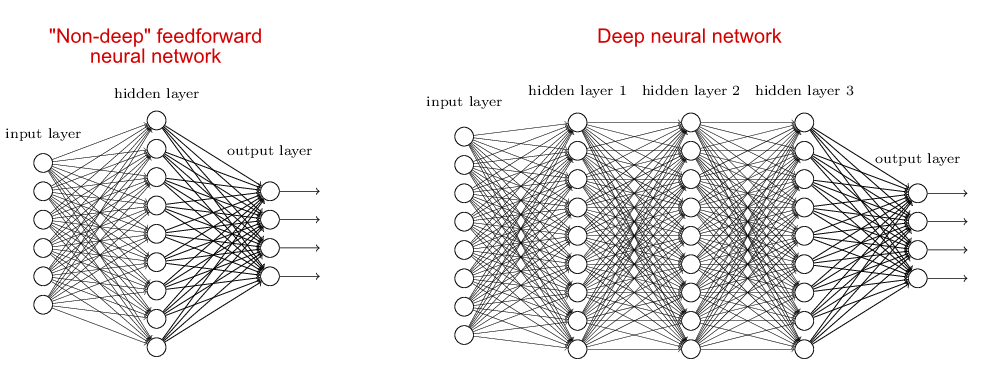
\includegraphics[width=0.9\textwidth]{dn.png}
  \caption{A shallow net and a deep net}
  \label{dn}
\end{figure}



For a data vector $x$: 

Construct a sequence of \emph{activation} vectors, $a^{[0]}, a^{[1]}, a^{[2]}, \ldots, a^{[L-1]}$, consisting of input, hidden layers, and output, as follows

\benum 
\item  \emph{Input}: 

$$ a^{[0]}  = x.$$

\item  \emph{Hidden layers}: The activations $a^{[1]}, a^{[2]}, \ldots, a^{[L-1]}$ are vectors constructed sequentially. Each is a vector, so $a_i^{[j]}$ is the $i$-th \emph{node} (or \emph{neuron} or \emph{unit}) in $j$-th layer. 

At every layer, the activations are computed in the following way: 

\benum 

\item First, a linear filtering is applied to the activations of the previous layer. 

$$z^{[i]} = W^{[i]}a^{[i-1]}+b^{[i]}.$$

This relies on the following parameters: $W^{[i]}$, $b^{[i]}$. For $i=1,\ldots$. The \emph{weights} $W$-s are matrices, while the \emph{biases} $b$-s vectors.

The resulting vectors $z$ are called \emph{pre-activations}.

The dimension of the activation can increase or decrease (e.g., compression, denoising) every layer. 

\item 
Next, a nonlinear \emph{activation function} $\sigma$ is applied coordinate-wise to the pre-activation vectors $z$: 

$$a^{[i]} = \sigma(z^{[i]}).$$


Popular examples: 

\bitem 
\item \emph{rectified linear unit} (ReLU): $\sigma(x) = \max(x,0)$. 
\item sigmoid: $\sigma(x) = 1/(1+\exp(-x))$. 
\eitem 

This can depend on $i$ and then it is denoted as $\sigma^{[i]}$. 


\item Output layer: 

$$\hat y = a^{[L]}.$$

For binary classification, the final layer is like a logistic regression. 

\eenum 


\eenum 
%The last layer's nonlinearity is chosen as a softmax for classification: $a^{[L]}_j = \exp(z^{[L]}_j)/[\sum_k\exp(z^{[L]}_k)]$.


\begin{figure}
  \centering
  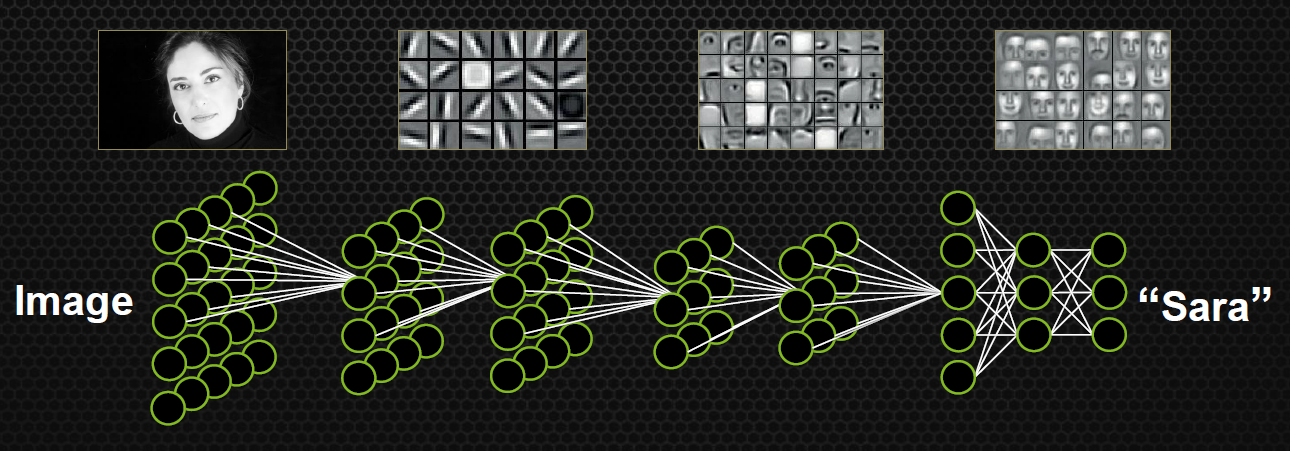
\includegraphics[scale=0.3]{nn_example.png}
  \caption{Example of feature learning.}
  \label{fl}
\end{figure}

\item Here are a few examples of deep learning visualizations to form intuition: 

Andrej Karpathy's tools for "Deep Learning in your browser
" \url{https://cs.stanford.edu/people/karpathy/convnetjs/}

Google's Neural Network Playground: \url{http://playground.tensorflow.org}


\item 
The intuition for neural networks is that they are able to extract \emph{higher-level features} of the data (Figure \ref{fl}). For instance 

\benum 
\item in the first layer, the weights can detect any linear combination of the input feature coordinates, (e.g., edges)
\item and then the activation function ensures that when there is a sufficient amount of that feature, it is propagated to the next layer. 
\eenum 


Moreover, the algorithms are thought to \emph{automatically learn} the optimal weights for accurate classification.  For instance in image classification, the lowest level features are often edge detectors, while the higher-level features look for combinations of edges in the right position, such as eyes in a face. 

The first examples of multilayer NNs, such as Fukushima's neurocognitron (1980) were tuned heuristically, without learning.

Before NNs, the state of the art in computer vision was to use any of a large number of libraries of features, combined with a linear  . Still very complicated, still heuristic.

\item Next, let us see how we can express the model with many training  examples. We will denote the training examples as $x^{[i]}$. We will also write for $a^{[j](i)}$ the $i$-th node corresponding to the $j$-th example. 

\benum 
\item 
\emph{Input layer}:  

$$A^{[0]} = X.$$ 
Here $X$ a matrix that has the training data as its columns. 

Matrix dimension: $n_x \times m$, where $n_x$ is dimension of samples (usually denoted by $p$ in statistics), and $m$ is number of samples (usually denoted by $n$ in statistics).
\item 
``\emph{Forward propagation}'': 

Activations $A^{[i-1]}$ arranged in a matrix. 

Matrices are organized as follows: columns - training examples/filters,  rows - units/nodes. 


$$Z^{[i]} =  W^{[i]}A^{[i-1]}+b^{[i]},$$

$$A^{[i]}  = \sigma(Z^{[i]})$$
\item  
\emph{Output layer}:  

$$\hat y = A^{[L]}.$$

There can be multiple outputs (e.g., center of car, width and height of the box enclosing it)

\eenum

\eenum

\subsection{Training}
\subsubsection{Backpropagation}

\benum
\item \emph{Loss function}: Consider only binary classification for simplicity. For one training example, we will use the \emph{logistic loss}: 

$$\ell(\hat y,y) = - y \log(\hat y) - (1-y) \log(1-\hat y)$$


e.g., if $y = 1$, loss is $\log(1/\hy)$ [plot]

For multiple training examples, consider the \emph{empirical risk}: 

$$J(W,b) = \frac{1}{m} \sum_{i=1}^m\ell(\hat y^{[i]},y^{[i]})$$

Here $\hat y$ are predictions of the neural network (defined above) with parameters $W  = (W^{[1]}, \ldots)$ and $b  = (b^{[1]}, \ldots)$. 

\item Training proceeds via \emph{gradient descent} (GD), or versions thereof. 

Fix some initialization of the parameters $W,b$, and a \emph{learning rate} $\alpha$. The parameters will be updated iteratively as 

$$W: = W - \alpha\, dW$$

$$b: = b - \alpha\, db$$

The convention is that for parameters $\theta$ we denote the Jacobian $d\theta: = \partial J/\partial\theta$. 

Technically, the loss may not be diffferentiable everywhere, if we use non-smooth nonlinearities such as ReLU. It turns out, that the probability of this being a problem is virtually non-existent with proper random initialization. 

\item We will show the form of GD for one data sample $x$. In practice, one would do it for a small randomly chosen data sample  (e.g., 256 images). This is known as \emph{mini-batch stochastic gradient descent} (SGD). One would vectorize the results as much as possible, for speed. 

We want to compute the derivatives of the empirical risk with respect to the weights $W^{[i]}$ and biases $b^{[i]}$. 

The computation proceeds backwards, starting from $dW^{[L]}$, and using the chain rule to compute $dW^{[i-1]}$ in terms of $dW^{[i]}$. Known as ``\emph{backpropagation}'',  (Rumelhart et al, 1986). Invented independently in several communities (e.g., ``adjoint state method'' in optimal control) and by several groups of researchers in neural networks (e.g, Sejnowski, LeCun) [Draw \emph{computation graph}]

\benum 
\item 
The last layer is special, because of the loss, and due to the use of the sigmoid: 

$$d W^{[L]} = \frac{\partial \ell(\hat y, y)}{\partial  W^{[L]}} = \frac{\partial \ell(\hat y, y)}{\partial  \hat y} \frac{\partial \hat y}{\partial  W^{[L]}}$$

Now 

$$\frac{\partial \ell(\hat y, y)}{\partial  \hat y} 
= - y\frac{ \log(\hat y)}{\partial  \hat y} - (1-y) \frac{ \log(1-\hat y)}{\partial  \hat y} 
= - \frac{y}{\hat y} + \frac{(1-y)}{1-  \hat y}$$

Also,

$$\frac{\partial \hat y}{\partial  W^{[L]}} 
=  \frac{\partial \sigma(z^{[L]})}{\partial  W^{[L]}} 
= \frac{\partial \sigma(z^{[L]})}{\partial  z^{[L]}}  \frac{\partial z^{[L]}}{\partial  W^{[L]}} $$

At the last layer, we use sigmoid $\sigma(x) = 1/(1+\exp(-x))$, with $\sigma'(x) = \sigma(x) (1-\sigma(x))$, so that 

$$dz^{[L]}= \frac{\partial \sigma(z^{[L]})}{\partial  z^{[L]}} =  \sigma(z^{[L]})(1-\sigma(z^{[L]})) = \hat y (1-\hat y)$$

From the two equations above we find the simplified form

$$\frac{\partial \ell(\hat y, y)}{\partial  z^{[L]}} = \hat y - y$$


Finally

$$ \frac{\partial z^{[L]}}{\partial  W^{[L]}} = \frac{\partial (W^{[L]} a^{[L-1]}+b^{[L]})}{\partial  W^{[L]}} = a^{[L-1]}$$


We also have, for the bias term, 

$$d b^{[L]} 
= \frac{\partial \ell(\hat y, y)}{\partial  b^{[L]}} 
= \frac{\partial \ell(\hat y, y)}{\partial  z^{[L]}}  \frac{\partial z^{[L]}}{\partial  b^{[L]}} $$

The first term was already computed, while the last term is the identity. 


This shows how to do backpropagation for the last layer. 


\item 
For the remaining layers, the calculation of $da^{[i-1]}, dz^{[i-1]}, \ldots $ is similar (and also the same calculation for all layers), assuming now that the derivatives $da^{[i]}, dz^{[i]}, \ldots $  for higher layers have been computed: 

$$d a^{[i-1]} 
= \frac{\partial \ell(\hat y, y)}{\partial  a^{[i-1]}} 
= \frac{\partial \ell(\hat y, y)}{\partial  z^{[i]}} \frac{\partial  z^{[i]}} {\partial  a^{[i-1]}}
= dz^{[i]}W^{[i]}$$

Also

$$d z^{[i-1]} 
= d a^{[i-1]}\frac{\partial  z^{[i-1]}}{\partial  a^{[i-1]}} = d a^{[i-1]}/ \sigma' (a^{[i-1]})$$

$$d W^{[i-1]} 
= d z^{[i-1]} a^{[i-1]}$$

and

$$d b^{[i-1]} = d z^{[i-1]}.$$

This shows how to do backpropagation for intermediate layers. 
\eenum 
\item The \emph{learning rate} hyperparameter $\alpha$ is chosen as a small value, such as $\alpha = 0.01$. 

\item See also \url{http://colah.github.io/posts/2015-08-Backprop/}


\eenum 
\subsubsection{Regularization}

\benum
\item The number of weights can be much larger than the sample size. Regularization is used to avoid overfitting. 

\item 
An \emph{$\ell_2$ penalty} is often used for regularization. Minimize

$$J(W,b) + \frac{\lambda}{2} \sum_{i=1}^L \|W^{[i]} \|_F^2$$

Also known as \emph{weight decay}, because the implementation reduces to 
$$W^{[i]}: = (1-\alpha/\lambda) W^{[i]} - \alpha\, dW^{[i]}$$

\item 
\emph{Dropout}: Randomly zero out units, to mitigate weight \emph{co-adaptation} (Srivastava et al 2014). 

At train time:  Draw masks for the activations with iid Bernoulli entries  $d^{[i]}$, say with success probability $q=0.8$: 

$$ d^{[i]}_j \sim_{iid} Bernoulli(q)$$

Zero out units:

$$a^{[i]} = a^{[i]}\odot d^{[i]}$$

Rescale, aka "\emph{inverted dropout}", in order to "not reduce the expected value of the next activation": 

$$a^{[i]} = a^{[i]}/q$$


Then keep the same iterations. This corresponds to freezing some randomly chosen weights at each iteration.

At test time: change nothing. 

Note: The original dropout applies rescaling at test time instead. 

\item 
\emph{Data augmentation}: Increase the sample size, by adding transforms of the training samples to the dataset. E.g., for images: random shift, zoom, small rotation, L-R flip, Random cropping, Shearing, Color shifting. 
\eenum 

\subsubsection{Other optimization steps}


\benum
\item \emph{Input normalization}. Normalize each feature of the input data to have unit norm. Reduces condition number of objective. 

\item 
Initialization: typically \emph{random initialization} is used. For instance, iid Gaussian weights, with some small variance. 

$$W^{[l]} \sim \N(0, \sigma^2_l \cdot I_{n_l}\otimes I_{n_{l-1}}).$$
 Here $\sigma^2_l$ is some function of the dimension and activation. For instance $$\sigma^2_l = 1/n_{l-1}$$ for linear and tanh (Xavier initialization). Also, $$\sigma^2_l = 2/n_{l-1}$$ for ReLU. These can work better than others such as $\sigma^2_l = 1/(n_l+n_{l-1})$.

\item \emph{Residual networks (ResNets)}, (He et al, 2015). Allow the information from a layer to ``skip'' a node.  Empirically, allow the training of much deeper networks. 

Recall that two layers of a feedforward network have the form

$$z^{[l+1]} = W^{[l+1]}a^{[l]}+b^{[l+1]}.$$

$$a^{[l+1]} = \sigma(z^{[l+1]}).$$

$$z^{[l+2]} = W^{[l+2]}a^{[l+1]}+b^{[l+2]}.$$

$$a^{[l+2]} = \sigma(z^{[l+2]}).$$

A residual network allows the information from a layer to ``skip'' a node: 

$$a^{[l+2]} = \sigma(z^{[l+2]}+ a^{[l]}).$$
 
The problem is that a linear transform $W^{[l+2]}a^{[l+1]}$ easily changes the ``magnitude'' of the activations. By adding the previous activations, we are now \emph{learning the residual}, and the baseline is the identity. This is easier. 

Training is very similar to before. 

\item Batch normalization (Ioffe \& Szegedy, 2015): Normalize the input to each layer to "prevent internal covariate shift".

\item Beyond SGD: There are several variants to accelerate SGD by adding a scaled difference of the previous steps: Adam (Kingma \& Ba, 2015), RMSProp (Hinton, 2012). See overview paper by Ruder. See Figure \ref{opt}.

\begin{figure}
  \centering
  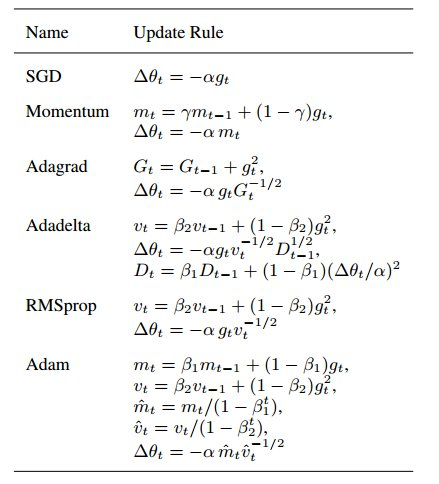
\includegraphics[scale=0.5]{opt}
  \caption{Optimization methods.}
  \label{opt}
\end{figure}



\item Scaling the input to be in a reasonable range, such as $[0,1]$.

\item Gradient clipping, elementwise. 


\eenum

\subsection{Notes on using DL}
\benum


\item  {\bf Flexibility.}

The input-output $x,y$ can be anything. This "\emph{black-box}" thinking gives a lot of flexibility to practitioners. The art is to reduce everything to supervised learning. How do you solve a problem using deep learning? You reduce it to $x,y$ pairs where $x$ is input, $y$ is output, and $y$ depends in a "smooth" way on $x$. \emph{Differentiable programming.}

 Examples:

\benum
\item
$y = x$. Known as an \emph{autoencoder} (Figure \ref{ae}). This is an example of \emph{unsupervised learning}. Denoises and compresses the input $x$ if we constrain the intermediate layers. 

\begin{figure}
  \centering
  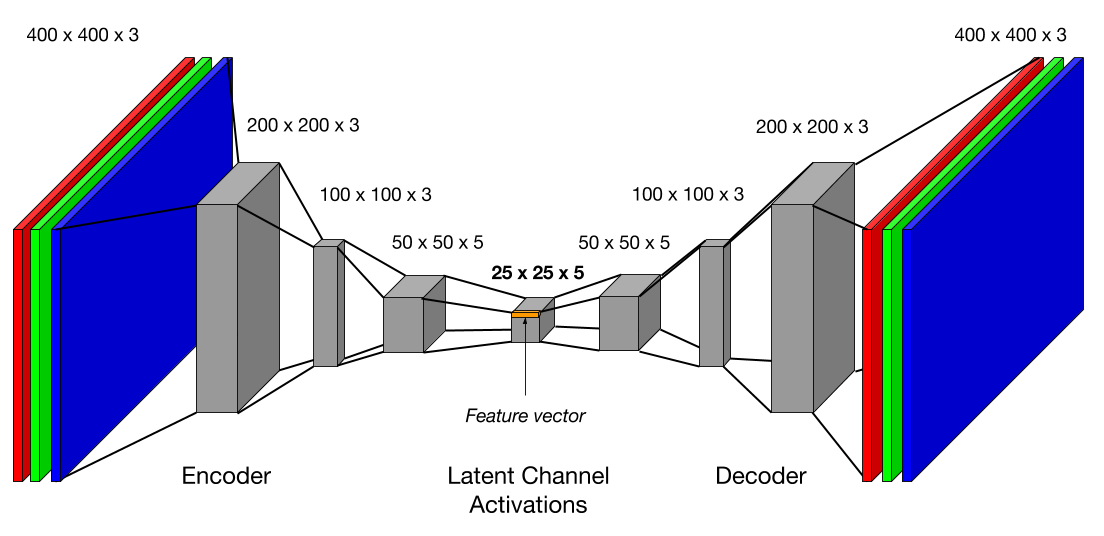
\includegraphics[scale=0.3]{ae.png}
  \caption{Autoencoder.}
  \label{ae}
\end{figure}




\item 
\emph{Object localization}: Input $x$ is an image. Output $y = (y_{center}, y_{height}, y_{width})$ is the position of a \emph{bounding box} containing an object (such as a car) in the image. Can also detect multiple objects.
 
\item Can transform data into images to make the existing techniques applicable (highly creative). For instance: 
\bitem 
\item Fraud detection: Mouse movement $\to$ image of  a line.

\item Genomics: Reads from a genome $\to$ image of colored dots. 
\eitem 
\eenum


\item {\bf What is so special about deep net architecture?} %Understanding architecture. 

%Can we think of another class of learning algorithms that does the same, except much better?

Purported special properties: 
\benum
\item
\emph{Universal approximators}. Can capture any structure, approximate any function. Deep $>$ shallow?
\item  \emph{Modular structure}. Can design architectures for any application, combining and reusing existing modules
\item \emph{Large capacity}. Performance keeps increasing with more data, doesn't saturate

\item \emph{No bias-variance tradeoff}. Bigger network reduces bias (also trains longer), \emph{but} more data reduces variance. So, there is no tradeoff. 
\eenum 


\item {\bf What else do we need for this to work?} Data and compute. 

\begin{figure}
  \centering
  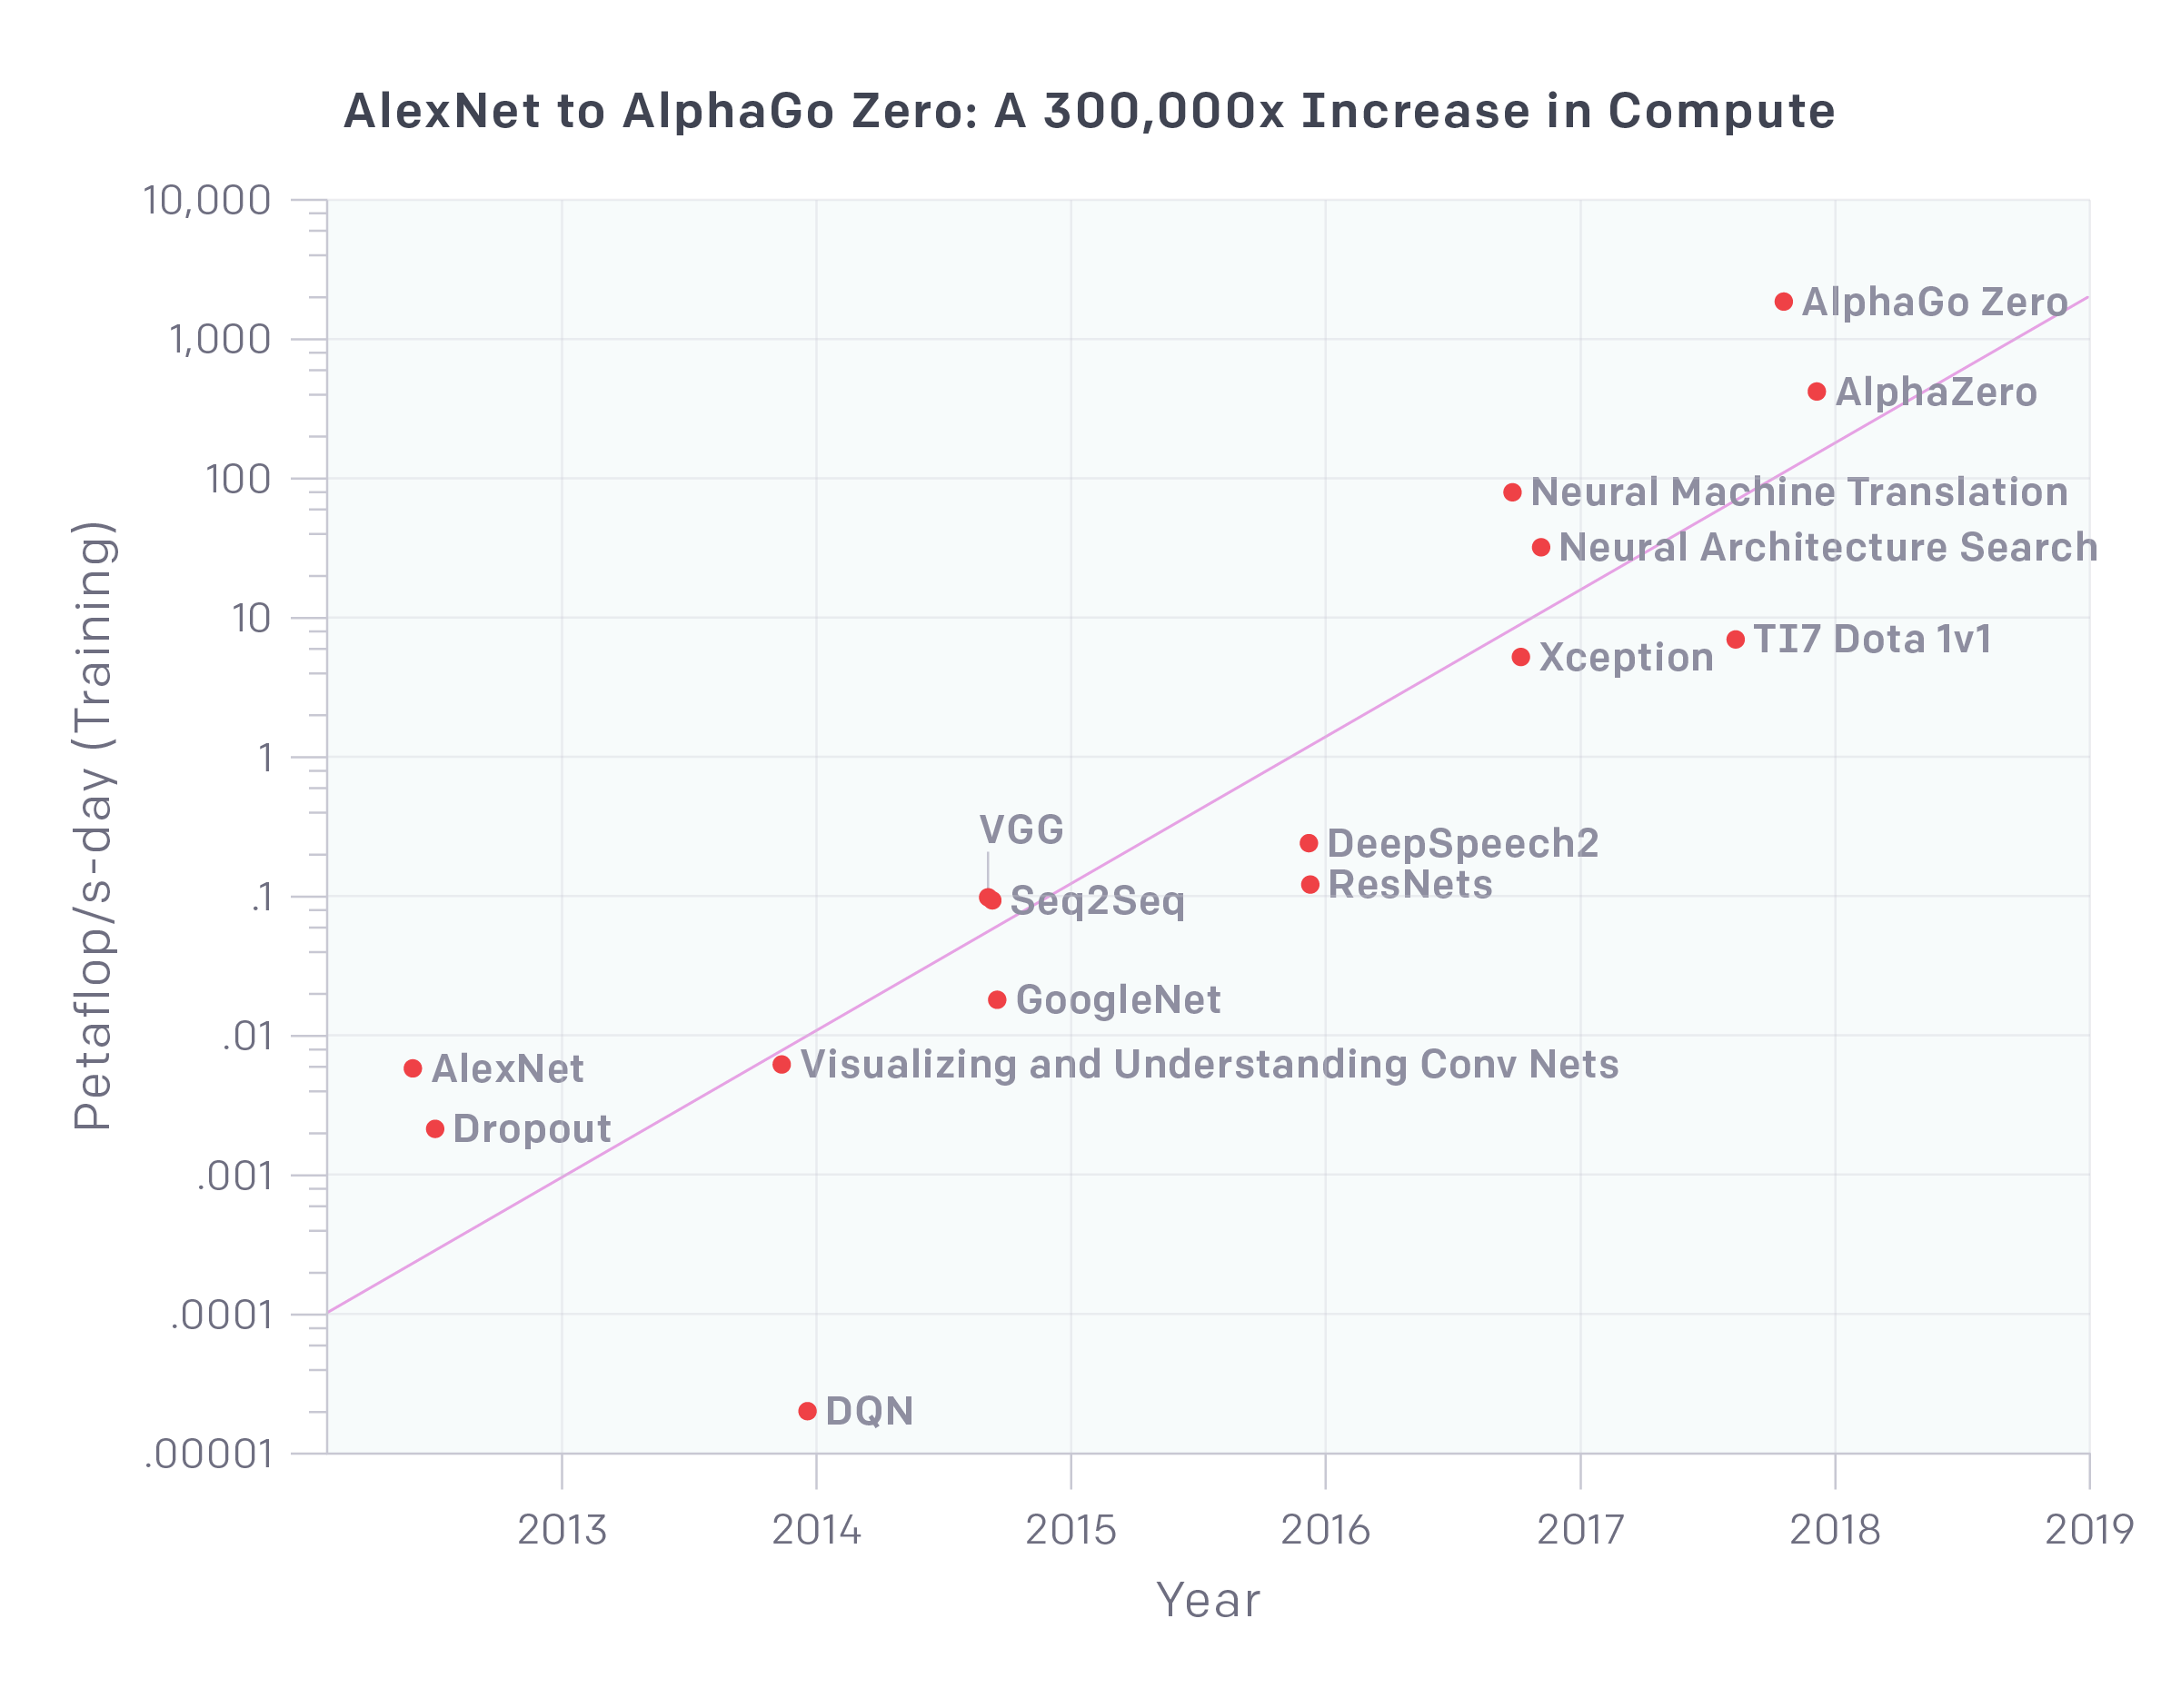
\includegraphics[scale=0.3]{compute_diagram-log@2x-3}
  \caption{AI and compute. \url{https://blog.openai.com/ai-and-compute/}.}
  \label{aic}
\end{figure}
%\item

Many research groups have reported good performance of deep neural networks for various problems. For instance the recent resurgence of interest in neural networks can be attributed to some extent to the 2012 paper by Krizhevsky, Sutskever, and Hinton, which  was able to achieve  good multi-class classification on the ImageNet dataset, with a specific type of convolutional neural network (CNN). 

The same type of CNN architecture had already been used since the 1980s, by many others including Hinton himself. The new success was mainly due to much larger  computational  resources available (including training on graphical processing units or GPUs), and much larger data sets available. The ImageNet dataset has millions of high quality  images. (See \url{https://www.kaggle.com/c/imagenet-object-localization-challenge})

\begin{quote}

It has only recently become possible to collect
\emph{labeled datasets with millions of images}''

``current \emph{GPUs}, paired with a highly-optimized implementation of 2D convolution, are powerful
enough to facilitate the training of interestingly-large CNNs''
\end{quote}

OpenAI, Figure \ref{aic}: 
\begin{quote}
Since 2012, the amount of compute used in the largest AI training runs has been increasing exponentially with a 3.5 month-doubling time.
\end{quote}

\item {\bf Economic value.}

NNs are also widely used for  \emph{online advertising}.  Specifically they are used to  predict  which ad to display to users to maximize  expected profits. It is thought that  most of the short-term \emph{economic value} that they generate  is from this area. This may not be a surprise given  that a large fraction of the revenue of internet companies like Google comes from online ads. 



\item {\bf Concerns in the community, and failures of deep learning.}

\benum 
\item
\emph{Self-driving car accident.}  Tesla autopilot crash: classifies truck as billboard. See Figure \ref{tes}.

\begin{figure}
  \centering
  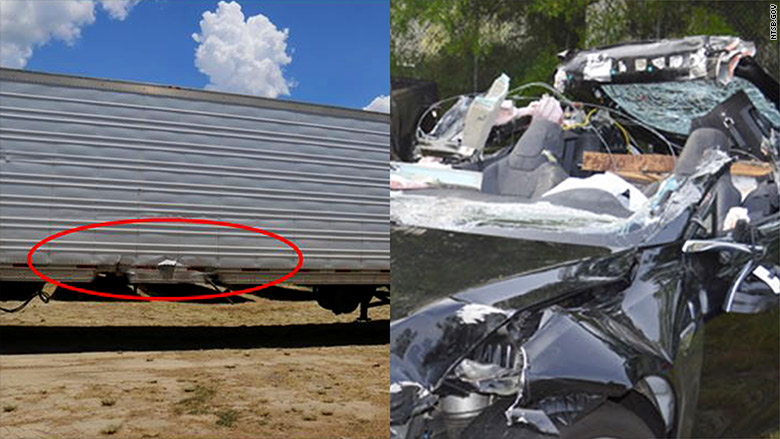
\includegraphics[scale=0.4]{tes}
  \caption{Tesla autopilot crash.}
  \label{tes}
\end{figure}
\item

\emph{Adversarial examples.} Add imperceptible image to panda, NN classifies it as gibbon with 99.9\% confidence. See Figure \ref{adv}.

\begin{figure}
  \centering
  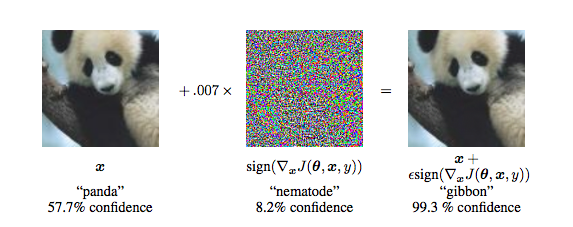
\includegraphics[scale=0.5]{goodfellow.png}
  \caption{Adversarial example.}
  \label{adv}
\end{figure}

Explanation: from \url{http://karpathy.github.io/2015/03/30/breaking-convnets/}.

Normal ConvNet training: “What happens to the score of the correct class when I wiggle this parameter?”

Creating fooling images: “What happens to the score of (whatever class you want) when I wiggle this pixel?”

We compute the gradient just as before with backpropagation, and then we can perform an image update instead of a parameter update, with the end result being that we increase the score of whatever class we want. 

\item

\emph{Reproducibility, finicky training.}   99 percent of work is: how to structure architecture correctly, how to tune parameters. Ali Rashimi, NIPS 2017, called it \emph{alchemy}: 

\begin{quote}
"How many times have you trained deep nets, and felt bad about yourself that they did not work? Wouldn't you like to know how batchnorm reduces internal covariate shift? Wouldn't you like to know what internal covariate shift \emph{is}?""
\end{quote}

\eenum


\item {\bf Automatic feature engineering.}

\benum 
\item The classical workflow in applications of supervised machine learning, statistics, data mining, etc., starts by thinking carefully about what features to use. 

E.g., Computer vision: Gist features. See Figure \ref{cv}.

\begin{figure}
  \centering
  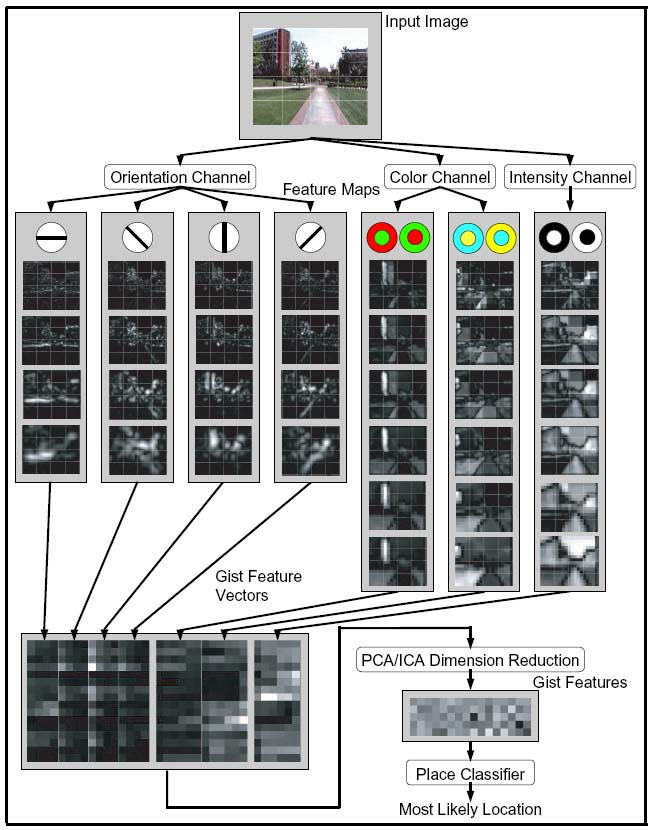
\includegraphics[scale=0.3]{Fig_GistExample}
  \caption{Computer vision features example.}
  \label{cv}
\end{figure}

\item This is (1) Time-consuming for humans, (2) Case-by-case, hard to automate, non-adaptive (3) Does not necessarily extract all information.

\item Deep learning replaces this by learning features automatically. (1) Less time-consuming for humans (even though computationally demanding), (2) Universal workflow, (3) Can always make network huge, and extract all information. 

\eenum 


\item {\bf Success criteria.}

\benum 
\item There is \emph{only one way} to succeed: reduce classification error. 
\item Even if this costs a lot of computation, and human labor. These are not always reported. 
\item Implications: 

"I proved a theorem" $\to$ Nobody cares.

"I proved a theorem, \emph{and} it helped me decrease classification error" $\to$ Lots of people care.


\eenum 


\item {\bf Workflow: first overfit, then regularize.}

\benum 
\item Deep nets are designed to squeeze out every bit of information in the data.
\item The workflow to do this is: \emph{first overfit, then regularize.}
\item In order for a class of machine learning models to be successful, it \emph{has to be able to overfit}. Otherwise, it leaves valuable information in the data. 

Overfit: Deeper network, wider network, more epochs

\item Regularize: smaller network, weight decay, dropout, smaller batch size, early stopping, lower learning rate, other hyperparameters

\eenum 


\eenum 


\subsection{Miscellanea}
\benum 
\item Who cares?
\bitem
\item Google, Facebook, Microsoft all have AI/Deep learning research groups. Thousands of projects use DL
\item More than 1300 DL startups as of 2017
\item Note: fake startup. Rocket AI. 

How many of the startups have no real basis? 
\eitem



\item Why?

\bitem
\item Large interest from industry, government, academia. Why?

\item Better-than-human (or just good) performance %at
\bitem
\item Computer vision: Classification, Segmentation, Caption generation, Object detection. Image processing: Inpainting, Superresolution, Style transfer (painting: Van Gogh, sketch to photo; design, Figure \ref{st})%(FB)

\begin{figure}
  \centering
  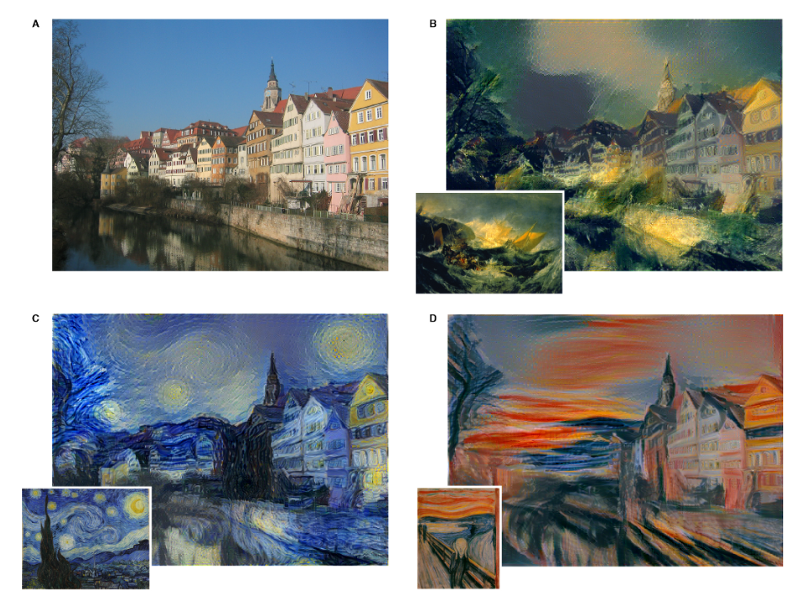
\includegraphics[scale=0.5]{st.png}
  \caption{Style transfer (Gatys et al 2015).}
  \label{st}
\end{figure}

\item Speech recognition: Voice commands, Video auto-cap, Real-time translation
\item Text analysis: Translation, Sentiment analysis (predict if review is positive)
\item Robotics: Self-driving cars
\item Fast fluid simulation, fast differential equation solvers.
\item Game playing: Go, Dota
\eitem
\item Potential to automate other tasks?
\item Note on better-than-human performance: Computers are already much better than human at many things. e.g. they have much better memory. Do math calculations. Communicate fast. Can be told what to do (and do it), by programming.


\eitem

\bitem
\item Can do things that were previously thought to be impossible for computers (even though they are trivial for humans)

Image Classification - humans can do it. But computers can do it faster, more systematically (and more versions). 

And, there are situations where insta-speed is needed.

This is the first step in scene understanding. When you think about an autonomous agent, it has to figure out where it is. 

It can be combined with other systems. Whenever you have a function that you fit to data, replace it with deep net. e.g., deep RL. any image processing task - deep version. 

Where is the opportunity?


\eitem



% \item  Applications to research? (Slightly tongue-in-cheek)

% \bitem
% \item How could it make \emph{my life} easier?
% \item Literature review. ``Is X known?'' %, ``What are the most used statistical methods recently?''
% \item No-typing paper writing. Style and grammar editing. 
% \item Analogy-based ideas ($\ell_1$: Lasso $\to$ group, GLM, adaptive, graphical, sparse PCA, fused, log-ratio)
% \eitem

\item Hardware: GPUs and cloud. Camera technology. Internet. Programming languages.

\item Software:  Keras. Tensorflow, PyTorch

\item Hype

\bitem
\item A lot of news coverage. "AI" captures public imagination %(one-second results, deep name). 
%\item Everybody knows about it, everybody talks about it
\item Many students are interested. "Default topic" for CS research. Typical paper at CS conference "We used DL for X, it worked great"

%"How did you decide not to do deep learning?"
\item "It can solve any problem". 
\eitem


\item Cautionary notes on the hype

\bitem
\item Humans have many \emph{cognitive biases} (see Tversky \& Kahneman, 2011 Nobel Prize in Economics)
\item \emph{Availability bias:} DL makes choosing research topic easy
\item \emph{Affect bias:} ``deep learning'' vs ``neural networks'' %Represent the, or even ``hierarchical local-convolution nonlinear approximation models''
\item \emph{Overconfidence:} ``AI revolution''
\item \emph{Neutral reference point:} take amazing things for granted
\item A lot of tuning in the background, dishonest presentation. "AI learns preiodic table in 8 hours"

"The 0.1\% mentality." At a big company, only need to improve tiny bit to keep job. Tuning is life. 
\eitem

\item 
Given the large hardware, power, and human \emph{costs} of the using neural networks it would be extremely valuable to have some guidance about when they are expected to work.  Many of the other algorithm that are deployed in applications are known to have a good performance under some  conditions. The value of these heuristics and results is that one can prioritize the algorithms and  save resources. 

Here are  a few widely used algorithms and statistical methods and the settings under which they are known to work: 

\benum
\item \emph{PageRank.} The core ranking algorithm used by Google's search engine, this is a linear algebra based method. The computational  convergence of the algorithm in guaranteed based on  strong results from numerical linear algebra. 

\item \emph{Linear regression.} This is a classical method for  prediction and statistical inference. The computation is based on simple linear algebra. The accuracy of the algorithm  for estimation is known in linear models. 

\eenum

In contrast there is much less known about the settings in which deep neural networks will work. We discuss some more specific questions below. 

\item {\bf Optimization.}

Simplest method (SGD) basically ``works''. How? Why is it so easy to optimize? Can it be made better? 

\item {\bf Generalization.}

Why not overfit? But: see concerns about overfitting to benchmark datasets. How can we reduce overfitting even more? 

Empirical observations in the paper by Zhang et al, ``Understanding DL requires rethinking generalization'', ICLR 2017

\benum
\item NNs fit everything. [This was not 100\% reproducible by other groups later.]

Classical learning theory does not apply. 

\item SGD is regularization

Other regularization doesn't help much

\item NNs are not stable

\item Optimization is  empirically easy even if the resulting model does not generalize. 

\eenum




\item  Comparing and contrasting deep learning and statistics. See also Figure \ref{mlai}

\begin{figure}
  \centering
  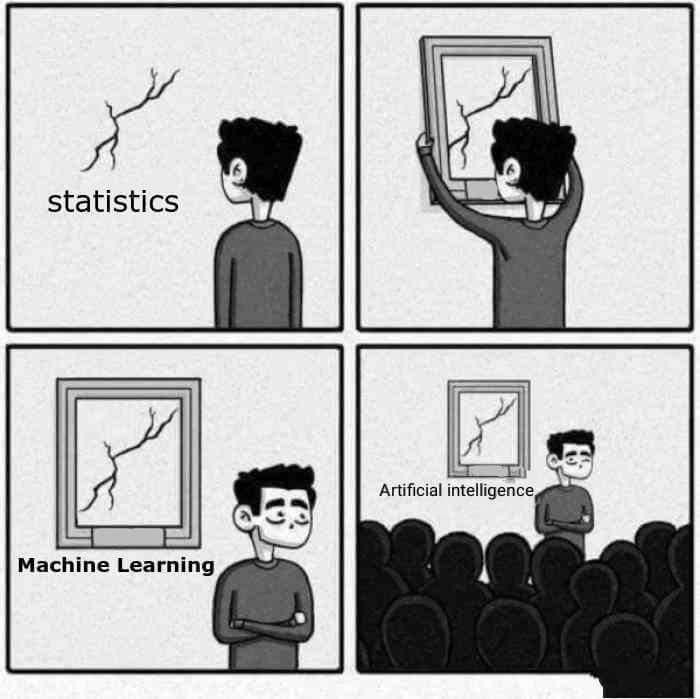
\includegraphics[scale=0.2]{mlai.jpeg}
  \caption{Statistics, ML, and AI. A humorous perspective.}
  \label{mlai}
\end{figure}

DL and stat both fit models, predict on data. However, the problems they address are very different: see Table \ref{my-label}.  

\renewcommand{\arraystretch}{1.5}
\begin{table}[]
\centering

\caption{DL and statistics}
\label{my-label}
\begin{tabular}{|l|l|l|}
\hline
                     & Deep learning & Statistics  \\ \hline
Sample size          & Huge          & Not too large       \\\hline  
Structure of Data       & High          & Varies      \\ \hline
Noise       & None          & Can be high      \\ \hline
Difficulty for human & Easy          & Can be hard \\ \hline
Computational Need        & Massive       & Varies      \\ \hline
Parameters    & As many as data          & Few        \\ \hline
Interpretability     & Low           & High        \\ \hline
Guarantees     & None           & Under assumptions        \\ \hline
Human tuning              & Effortful     & Easy        \\ \hline
Overall Cost         & High          & Lower         \\ \hline
\end{tabular}
\end{table}

%programming languages
\item  Limitations: 

People don't learn like that

There are many documented examples (and many more undocumented ones), where simpler methods work better. 

Dexterity and manipulation 

They are not intelligent!


\item Thought leaders in the tech world all bet on AI: 

Bill Gates:

\begin{quote}
What technology are you most looking forward to in the next 10 years and what impact do you think it could have?

Bill Gates:
The most amazing thing will be when computers can read and understand the text like humans do. Today computers can do simple things like search for specific words but concepts like vacation or career or family are not "understood". Microsoft and others are working on this to create a helpful assistant. It has always been kind of a holy grail of software particularly now that vision and speech are largely solved. Another frontier is robotics where the human ability to move and manipulate is amazing and experts disagree on whether it will take just a decade or a lot longer (Brooks) to achieve the equivalent.
\end{quote}

Jeff Bezos:

\begin{quote}
Embrace External Trends

The outside world can push you into Day 2 if you won’t or can’t embrace powerful trends quickly. If you fight them, you’re probably fighting the future.
Embrace them and you have a tailwind.
These big trends are not that hard to spot (they get talked and written about a lot), but they can be strangely hard for large organizations to embrace. We’re in
the middle of an obvious one right now: machine learning and artificial intelligence.
Over the past decades computers have broadly automated tasks that programmers could describe with clear rules and algorithms. Modern machine learning
techniques now allow us to do the same for tasks where describing the precise rules is much harder.


Inside AWS, we’re excited to lower the costs and barriers to machine learning and AI so organizations of all sizes can take advantage of these advanced techniques.

Watch this space. Much more to come.
\end{quote}



\item Intrepretability: excellent reference \url{https://distill.pub/2018/building-blocks/}

\item Creative architecture design, Figure \ref{arch}


\begin{figure}
  \centering
  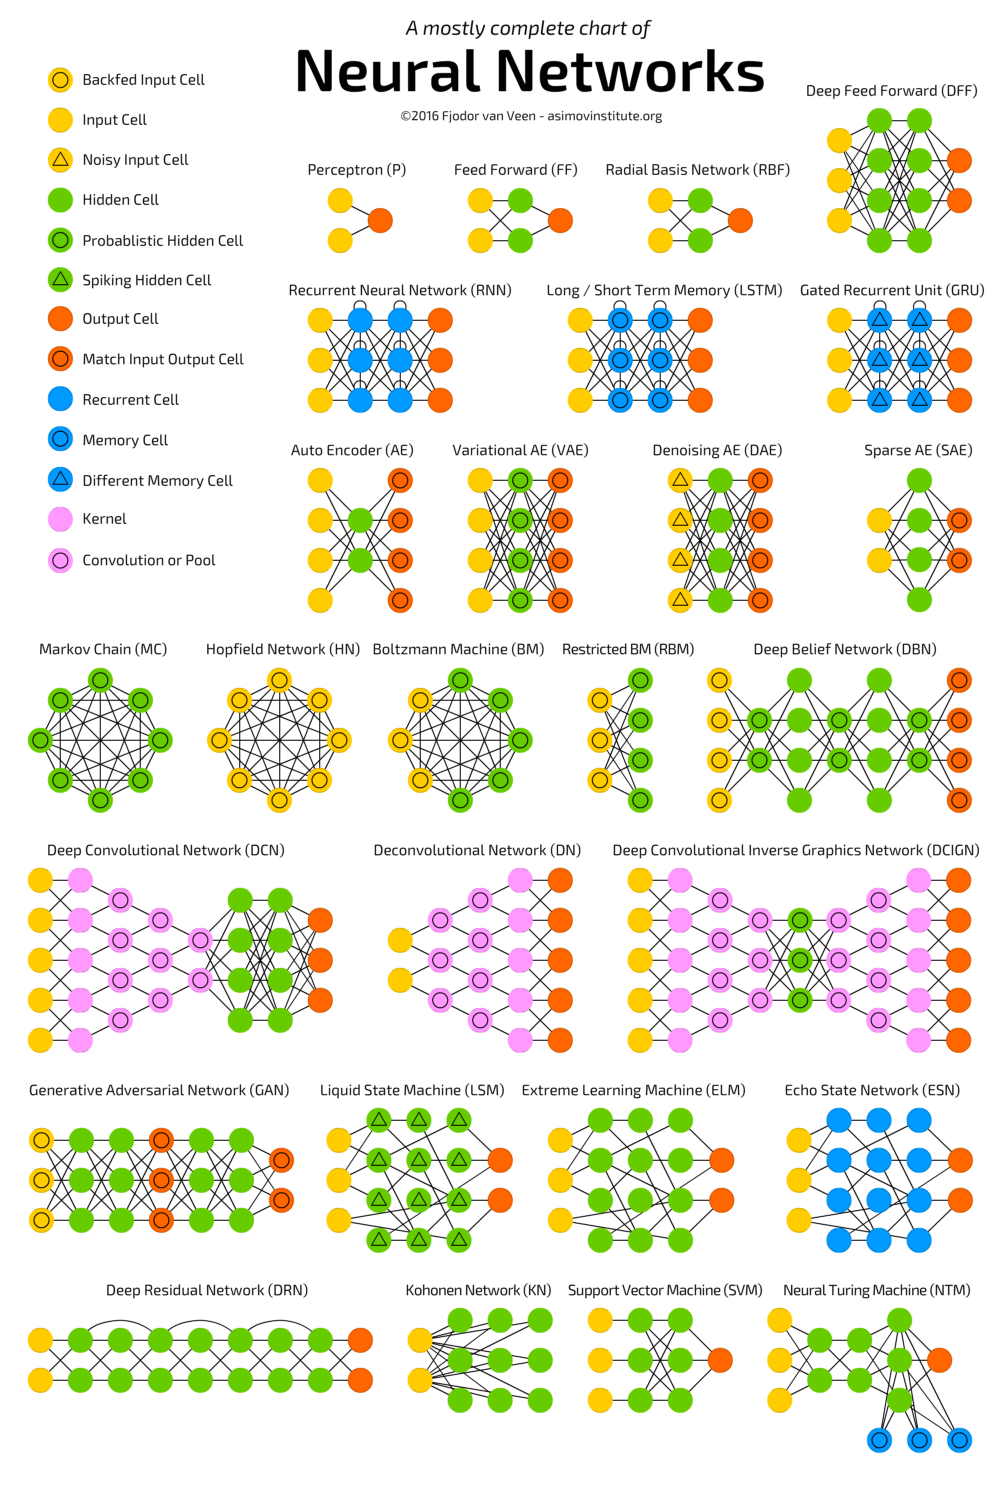
\includegraphics[scale=0.35]{Chart.png}
  \caption{Creative architectures.}
  \label{arch}
\end{figure}

%\item Naming: ...Net, Deep...

\eenum



\section{Convolutional neural networks (CNNs)}
\subsection{The problem and model}
\benum
\item Real data has structure. Nets can exploit this. e.g., images have a lot of structure: always a small number of objects, composed of smaller objects, strong correlations between pixels. 


Computer vision
\benum
\item \emph{Image classification}: e.g., recognize faces 
\item \emph{Object detection}: e.g., find cars in an environment
\item \emph{Style transfer}: e.g., design new objects based on existing styles (Figure \ref{st})

\eenum
Image dimensions are very large, so fully connected networks have too many parameters. \emph{Convolutional neural networks (CNNs)} are used instead. They exploit the "structure" of natural images in a more efficient way. 

\item \emph{Image} $X$: $n\times n$. e.g., an image of a road scene with cars.

\item \emph{Convolutional Layer:} The structure of a convolutional layer is as follows

\benum 
\item 
\emph{Filter} $F$: $ f\times f$ image, of small size, $3 \times 3$, $5 \times 5$, etc. e.g., an edge detector.

The \emph{convolution} operation is denoted as 
$$X * F$$

This takes all possible inner products of $F$ with \emph{patches} of $X$. It creates an $(n-f+1) \times (n-f+1)$ image.

Formally, an entry $i,j$ of $X * F$ is defined as $$X * F[i,j]=\tr \left\{X[i:i+f-1,j:j+f-1] \cdot F \right\}$$ 

(where $A\cdot B$ is the usual matrix multiplication)

Easy to extend to ``\emph{tensors}'', where you have several \emph{channels} of an image (e.g., color channels). A filter has the same depth as the number of channels of the previous layer, and the inner products are computed and summed over all channels.

\item \emph{Padding}: 

Pad outside of $X$ with zeros to keep the dimension of images fixed. 

After padding with $p$ zeros, the output is $(n+2p-f+1) \times (n+2p-f+1)$

Filter size is usually chosen as an odd integer, so we can pad with $p = (f-1)/2$ pixels everywhere, to keep the dimension of images fixed. 

\item \emph{Strided convolutions}:

Jump over some steps, so restrict to $X * F[i,j]$ to $i,j=1,1+s,1+2s,\ldots$.
Then the output will have size $\lfloor \frac{n+2p-f+1}{s}\rfloor \times \lfloor \frac{n+2p-f+1}{s}\rfloor$

\item Usually take multiple filters. These become the channels in the next layer. With an image of size $n \times n \times L$, and $k$ layers of size 
$f \times f \times L$, get  an output tensor of size $(n-f+1) \times (n-f+1) \times k$ 


Number of parameters is much smaller than for fully connected networks. ``Parameter sharing'', sparse connections. %(Invariance?)

Why convolutions? Vaguely related to local translation invariant structure of images, and \emph{symmetry}. %See papers by Mallat, Bolcskei etc.  
More precisely?


\item Then, add bias and apply ReLU. 
 
In deep networks, in the first layers typically we keep an equal height and width, and add more channels. Then reduce H/W, by increasing stride. %The last few layers are typically fully connected (FC), e.g., 4096-dimensional.

\begin{figure}
  \centering
  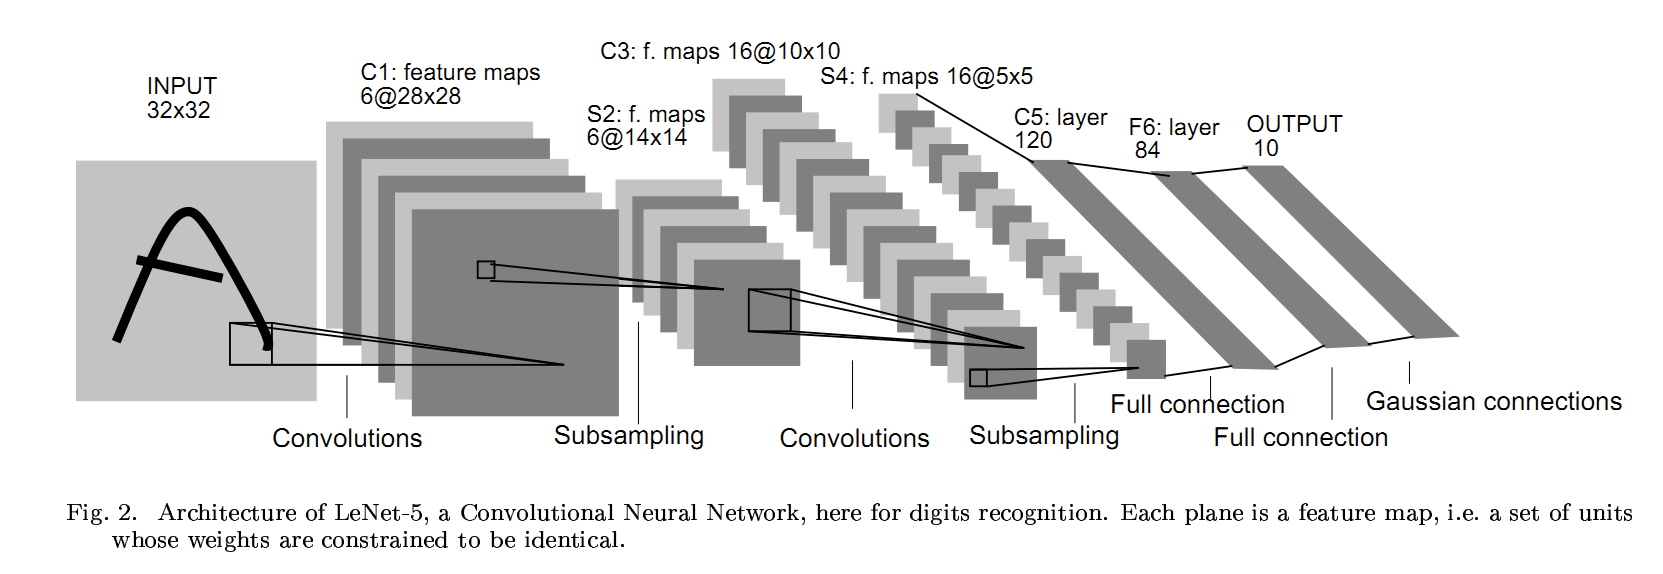
\includegraphics[scale=0.3]{lenet.png}
  \caption{LeNet-5. (LeCun, 1998)}
  \label{lenet5}
\end{figure}


\begin{figure}
  \centering
  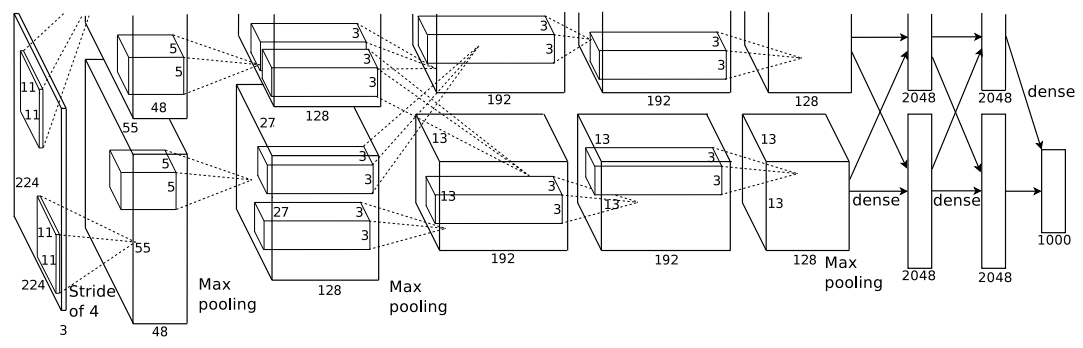
\includegraphics[scale=0.75]{a.png}
  \caption{AlexNet. Krizhevsky et al (2012, NIPS), Won ILSVRC 2012.}
  \label{AlexNet}
\end{figure}


\begin{figure}
  \centering
  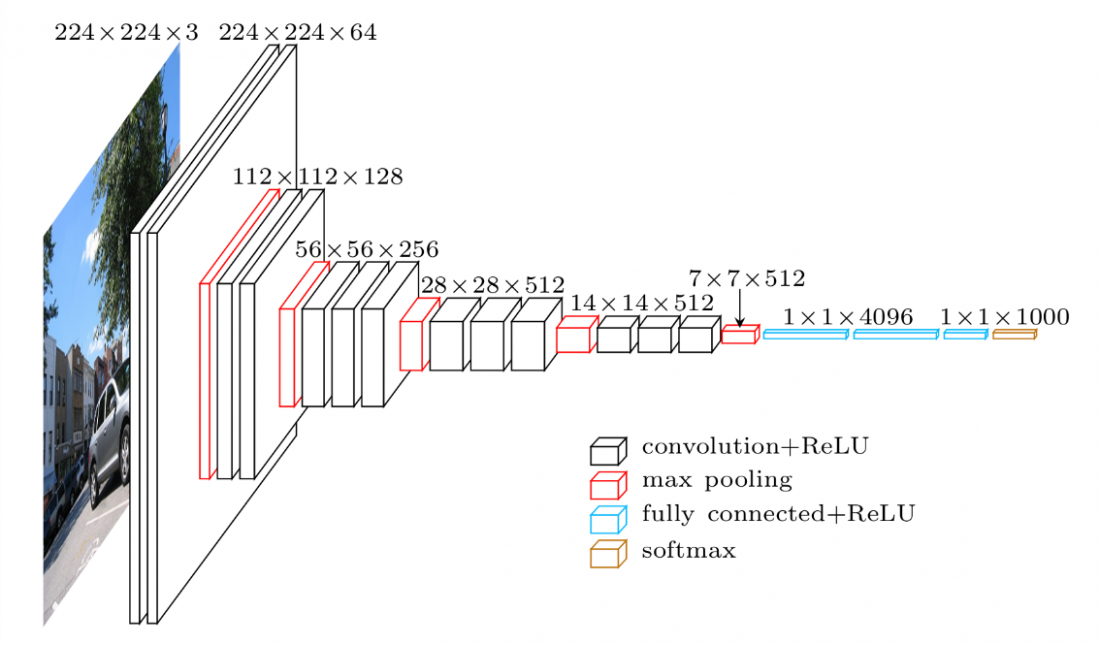
\includegraphics[scale=0.3]{vgg.png}
    \caption{VGG. (Simonyan, Zisserman, 2015).}
    \label{VGG}
\end{figure}

\eenum 



\item \emph{Pooling.} Reduces dimension of an image by ``pooling'' across neighboring activations. 

\emph{Max-pooling} with parameters $f$, $p$

$$X_P[i,j]=\max_{i\le k \le  i+f-1 ,j \le l \le j+f-1} X[k,l]$$ 

And restrict to $i,j=1,1+s,1+2s,\ldots$.

\emph{Average-pooling} used to be popular, but the non-linear max pooling seems to work better recently. 

\item The last few layers are typically fully connected.

Simple example: ``\emph{LeNet}'' type networks, starting from 1980s (Figure \ref{lenet5}). 

More recent examples: AlexNet (Figure \ref{AlexNet}). VGG (Figure \ref{VGG}). 

\item Visualize NNs, by finding images that maximize activation: hallucinogenic images (Figure \ref{vis}).

\begin{figure}
  \centering
  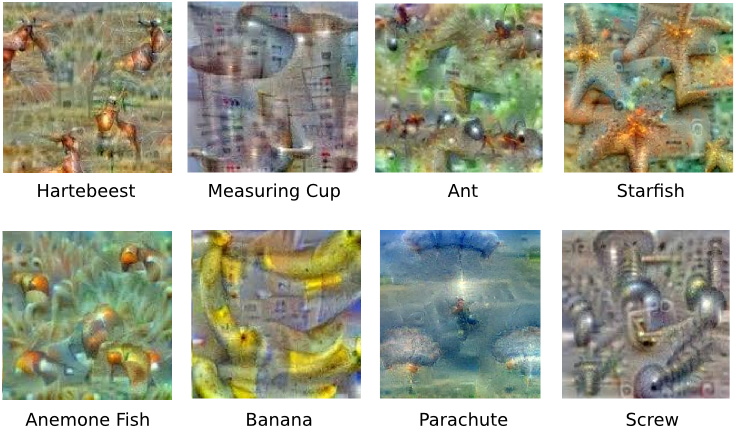
\includegraphics[scale=0.7]{vis.png}
    \caption{Images that maximize activation. The neurons selected for these images are the output neurons that a DNN uses to classify images as bananas etc.}
    \label{vis}
\end{figure}

\item Excellent reference on feature visualization: \url{https://distill.pub/2017/feature-visualization/}

Live demo of digit visualization: \url{http://scs.ryerson.ca/~aharley/vis/conv/}


\item See also \url{http://colah.github.io/posts/2014-07-Conv-Nets-Modular/}, 

\url{http://colah.github.io/posts/2014-07-Understanding-Convolutions/}

Yosinski's Deepvis toolbox: \url{http://yosinski.com/deepvis}
\eenum



\subsection{Other aspects}
\benum
\item R-CNN: Regions with CNN features (Girshick et al, 2013, Rich feature hierarchies for accurate object detection and semantic segmentation). Figure \ref{rcnn}.


\begin{figure}
  \centering
  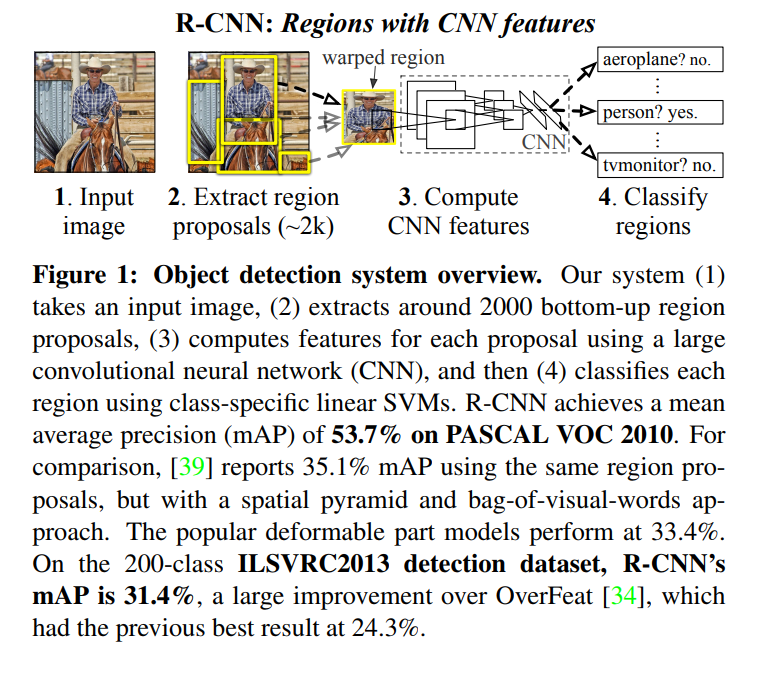
\includegraphics[scale=0.7]{rcnn.png}
    \caption{R-CNN.}
    \label{rcnn}
\end{figure}

Relies on "Selective Search for Object Recognition", Uijlings, van de Sande (2013) for region proposal.

Once the proposals are created, R-CNN warps the region to a standard square size and passes it through to a modified version of AlexNet (the winning submission to ImageNet 2012 that inspired R-CNN), as shown above.

On the final layer of the CNN, R-CNN adds a Support Vector Machine (SVM) that simply classifies whether this is an object, and if so what object. This is step 4 in the image above.

Later: Fast R-CNN, Mask R-CNN. See  

\url{https://blog.athelas.com/a-brief-history-of-cnns-in-image-segmentation-from-r-cnn-to-mask-r-cnn-34ea83205de4}
\eenum

\subsection{Training}
\benum
\item In principle, training proceeds in the same way via backpropagation
\item \emph{Transfer learning} is an important way to reduce computational cost. You can use the first layers a pre-trained standard architecture (such as VGG-19) as the starting point of your architecture. You can extend it to suit your problem by adding new layers. 

It is often observed that the features learned on one task, such as ImageNet classification, can be quite transferable to other problems, such as image segmentation. 

\item \emph{Data Augmentation.} Done in a streaming fashion. 

\emph{Mirroring, Shifting, Random cropping}. Also: \emph{Rotation, Shearing}

\emph{Color shifting}. From the AlexNet paper: 


\begin{quote}
Specifically, we perform PCA on the set of RGB pixel values throughout the
ImageNet training set. To each training image, we add multiples of the found principal components,
with magnitudes proportional to the corresponding eigenvalues times a random variable drawn from
a Gaussian with mean zero and standard deviation 0.1.
\end{quote}


\begin{quote}
This scheme approximately captures an important property of natural images,
namely, that object identity is invariant to changes in the intensity and color of the illumination.
\end{quote}
\eenum



\subsection{Graph CNN}
%
\bitem
\item Convolutional Neural Networks are efficient architectures in image and
audio recognition tasks, thanks to their ability to exploit the local translational
invariance of signal classes over their domain. How about signals defined on more general domains?

\item 3.1 Graph Signal Processing.


"The emerging field of GSP aims at bridging the gap between signal processing and spectral graph theory, a blend between graph theory and harmonic analysis. A goal is to generalize
fundamental analysis operations for signals from regular grids to irregular structures embodied by
graphs. Standard operations on grids
such as convolution, translation, filtering, dilatation, modulation or downsampling do not extend
directly to graphs and thus require new mathematical definitions while keeping the original intuitive
concepts."

D. Shuman, S. Narang, P. Frossard, A. Ortega, and P. Vandergheynst. The Emerging Field of Signal
Processing on Graphs: Extending High-Dimensional Data Analysis to Networks and other Irregular Domains. 2013.

\item From Bruna, Zaremba, Szlam, LeCun "Spectral Networks and Deep Locally Connected Networks on Graphs" (2014)

On a regular grid, a CNN is able to exploit several structures that play nicely together to greatly
reduce the number of parameters in the system:

\bitem 
\item  The translation structure, allowing the use of filters instead of generic linear maps and
hence weight sharing.
\item  The metric on the grid, allowing compactly supported filters, whose support is typically
much smaller than the size of the input signals.
\item  The multiscale dyadic clustering of the grid, allowing subsampling, implemented through
stride convolutions and pooling.
\eitem 


In many contexts, however, one may be faced with data defined over coordinates which lack some,
or all, of the above geometrical properties. For instance, data defined on 3-D meshes, such as
surface tension or temperature, measurements from a network of meteorological stations, or data
coming from social networks or collaborative filtering, are all examples of structured inputs on which
one cannot apply standard convolutional networks. Another relevant example is the intermediate
representation arising from deep neural networks. Although the spatial convolutional structure can
be exploited at several layers, typical CNN architectures do not assume any geometry in the “feature”
dimension, resulting in 4-D tensors which are only convolutional along their spatial coordinates.

\item Spatial Construction

\bitem 

\item Local, multiscale, hierarchical,

\item Graph $G = (\Omega, W)$. Vertices $\Omega$ are a set of size $m$, and edge weights are collected in an  $m\times m$ nonnegative matrix  $W$

\item Local: Neighborhood $N_\delta(j) = \{i:W_{ij}>\delta\}$. Use only filters restricted to neighborhoods.

\item Multiscale: "In this work we will use a naive agglomerative method."

\item Hierarchical: Exactly what you think

\eitem 


\item Spectral Construction

\bitem 

\item Combinatorial Laplacian: $L = D-W$, where $D = \diag(W1)$ is the diagonal matrix of degrees. 

Graph Laplacian $\mathcal{L} = I-D^{-1/2}WD^{-1/2}$. 

\item Smoothness functional for signal $x$ on graph:

$$\|\nabla x\|_W^2(i) = \sum_j W_{ij} [x(i)-x(j)]^2$$

So 

$$\|\nabla x\|_W^2 
= \sum_{i,j} W_{ij} [x(i)-x(j)]^2
= 2x^\top L x
$$


\item Global min: $v_0 = m^{-1/2}1$.

Successive minima: 

$$v_i =\arg\min_{x\in\R^m, x\perp{v_j}, j<i} 
\frac{\|\nabla x\|_W^2}{\|x\|^2}
$$
Eigenvectors of $L$ with eigenvalues $\lambda_i$ "allow the smoothness of a vector to be read off
from the eigenvalues, equivalently as the Fourier coefficients of a signal defined
in a grid. Thus, just an in the case of the grid, where the eigenvectors of the Laplacian are the
Fourier vectors, diagonal operators on the spectrum of the Laplacian modulate the smoothness of
their operands."

\item "3.2 Extending Convolutions via the Laplacian Spectrum"

Given a weighted graph, we can try to
generalize a convolutional net by operating on the spectrum of the weights, given by the eigenvectors of its graph Laplacian.


\bitem 

\item Start with $K$ layers, transforming input vectors $x_k$ of size $m\times f_{k-1}$ to output $x_{k+1}$ of size $m\times f_{k}$ (no spatial subsampling)

$$
x_{k+1,j}
= \sigma 
(
V \sum_{i=1}^{f_k} F_{kij} V^\top x_{ki}
)
$$

where $V$ is the matrix of eigenvectors of $L$, and $F_{kij}$ is a diagonal matrix. 

\item Issues:  most graphs have meaningful eigenvectors only for
the very top of the spectrum
\eitem 

\item "3.3 Rediscovering standard CNNs". A simple, and in some sense universal, choice of weight matrix in this construction is the covariance
of the data. It turns out that with this weights, gNN approximately recovers CNN.


\item Spatial locality: Smoothness in the spectral domain. "A particularly simple and naive choice consists in choosing a 1-dimensional arrangement, obtained
by ordering the eigenvectors according to their eigenvalues.  In this setting, the diagonal of each filter
$F_{kij}$ (of size at most $m$) is parametrized by

$$diag(F_{kij}) = K\alpha_{kij}$$

where $K$ is a $d \times q_k$ fixed cubic spline kernel and $\alpha_{kij}$ are the spline coefficients.




\eitem 

\item Improvements: "Convolutional Neural Networks on Graphs
with Fast Localized Spectral Filtering" Michaël Defferrard, Xavier Bresson, Pierre Vandergheynst. (Figure \ref{gcnn})


\begin{figure}
  \centering
  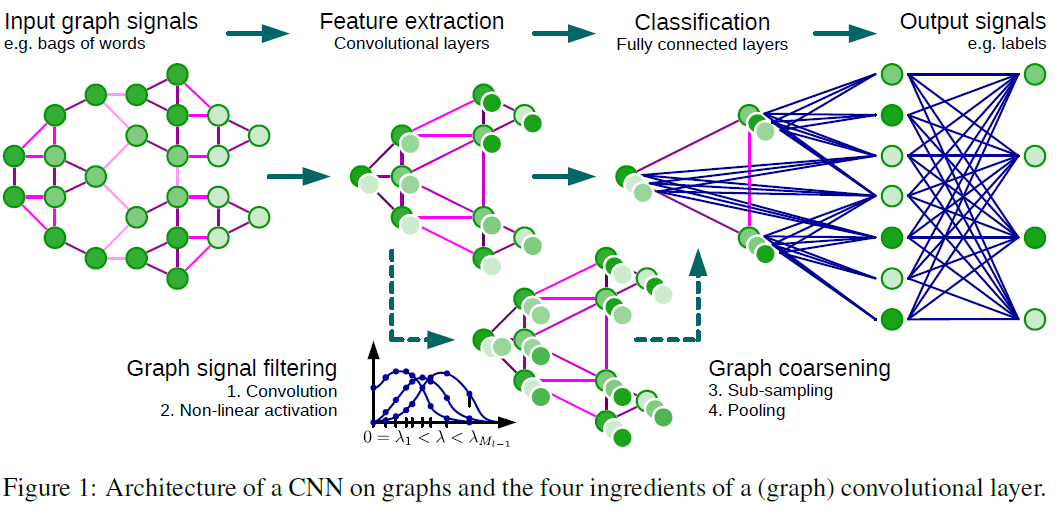
\includegraphics[scale=0.5]{gcnn.png}
    \caption{Graph CNN.}
    \label{gcnn}
\end{figure}



\benum 
\item 
Limitations: "the dominant cost is the need
to multiply the data by U twice (forward and inverse Fourier transforms)". "no precise control over the
local support of their kernels"

\item 2 Proposed Technique

Generalizing CNNs to graphs requires three fundamental steps: (i) the design of localized convolutional filters on graphs, (ii) a graph coarsening procedure that groups together similar vertices and
(iii) a graph pooling operation that trades spatial resolution for higher filter resolution.

\item They parametrize the filters $F$ as polynomials of the eigenvalues, $g_\theta(\Lambda) = \sum_{k=0}^{K-1} \theta_k \Lambda^k$, where $\Lambda$ is the diagonal matrix of eigenvalues of the laplacian. 

Spectral filters represented by K-th order polynomials of the Laplacian are exactly K-localized.

\item Moreover, to compute it efficiently, use a recurrence like Chebyshev polynomials. 

\item Training. Todo.

\begin{align*}
y &= g_\theta(L) x\\
&= \sum_{k=0}^{K-1}\theta_k T_k(\tilde L)x\\
&=[\bar x_0, \ldots, \bar x_{K-1}]\theta
\end{align*}


The $j$-th output feature map  the sample $s$ is given by

$$y_j = \sum_{i=1}^{F_{in}} g_{\theta_{ij}}(L) x_{si} $$


where the $x_{si}$ are the input feature maps and the $F_{in} \times F_{out}$ vectors of Chebyshev coefficients $\theta_{ij} \in \R^K$ are the layer’s trainable parameters. When training multiple convolutional layers with the backpropagation algorithm, one needs the two gradients

$$
\partial E/\partial{\theta_{ij}}
=
\sum_{s=1}^S
[\bar{x}_{s,i,0} ,\ldots, \bar{x}_{s,i,K-1}]^T
\partial E/\partial{\theta_{ij}}
$$
and 
$$
\partial E/\partial{x_{si}}
=
\sum_{j=1}^{F_{out}}
 g_{\theta_{ij}}(L)
\partial E/\partial{y_{sj}}
$$
where $E$ is the loss energy over a mini-batch of $S$ samples. Each of the above three computations boils down to K sparse matrix-vector multiplications and one dense matrix-vector multiplication for
a cost of $O(K|E|F_{in} F_{out} S)$ operations. These can be efficiently computed on parallel architectures
by leveraging tensor operations.


\item 2.2 Graph Coarsening. (Figure \ref{gcp})

\begin{figure}
  \centering
  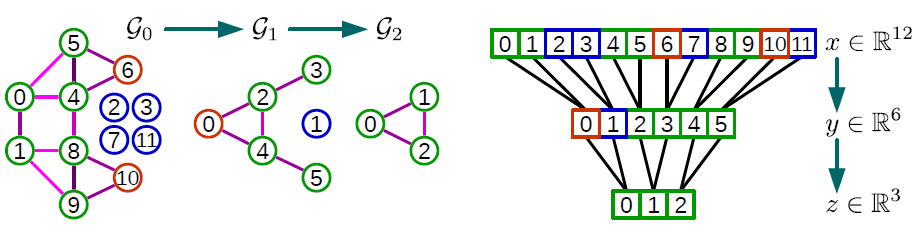
\includegraphics[scale=0.5]{gcp.png}
    \caption{Graph Coarsening and Pooling.}
    \label{gcp}
\end{figure}


Graclus [9], built on Metis [16], uses a greedy algorithm to compute successive coarser versions of a given graph and is able to minimize several popular spectral clustering objectives, from which we chose the normalized cut [30].

Graclus' greedy rule consists, at each coarsening level, in picking an
unmarked vertex i and matching it with one of its unmarked neighbors j that maximizes the local normalized cut $W_{ij} (1/d_i + 1/d_j)$. The two matched vertices are then marked and the coarsened weights are set as the sum of their weights. The matching is repeated until all nodes have been explored.  [Form of hierarchical clustering.]

\item 2.3 Fast Pooling of Graph Signals

Pooling operations are carried out many times and must be efficient. After coarsening, the vertices
of the input graph and its coarsened versions are not arranged in any meaningful way. Hence, a
direct application of the pooling operation would need a table to store all matched vertices. That
would result in a memory inefficient, slow, and hardly parallelizable implementation. It is however
possible to arrange the vertices such that a graph pooling operation becomes as efficient as a 1D
pooling. We proceed in two steps: (i) create a balanced binary tree and (ii) rearrange the vertices.

\eenum 

\item Convolutional Neural Network Architectures for
Signals Supported on Graphs, Gama, Marques, Leus, Ribeiro. 2018.

SELECTION GRAPH NEURAL NETWORKS

Graph $G$ with nodes $n$

Features $x_0^f$, (or just $x$, with entries $x_n$ at node $n$)

Filters $h_1^{fg}$ (vectors of arbitrary dimension $K$) 

Shift
operator $S$, which is a square matrix having the same
sparsity pattern of the graph; i.e., we can have $S_{mn}\neq 0$ if
and only if $(n,m) \in E$ or $m = n$. The shift operator is a
stand in for one of the matrix representations of the graph.
Commonly used shift operators include the adjacency matrix
$A$ with nonzero elements $A_{mn} = W(n,m)$ for all $(n,m) \in
E$, the Laplacian $L := diag(A1) - A$ and their normalized
counterparts.


Intermediate features $u_1^{fg}$ with components

$$
[u_1^{fg}]
:=
[h_1^{fg}*_Sx_0^g]_n
:=
\sum_{k=0}^{K_1-1}
[h_1^{fg}]_k[S^kx_0^f]_n
$$

where we have used $*_S$ to denote the graph convolution
operation on S.

The graph filter is a generalization of the Chebyshev filter
in Deferrard et al. More precisely, if G is an undirected graph, and we
adopt the normalized Laplacian as the graph shift operator S,
then it boils down to a Chebyshev filter.

A. Selection Sampling on Graph Convolutional Features

The challenge in generalizing CNNs to GNNs arises beyond
the first layer. After implementing the sampling operation, the signal is of lower dimensionality  and
can no longer be interpreted as a signal supported on S.

 Resolving mismatched supports is a well-known
problem in signal processing whose simplest and most widely-
used solution is zero padding. 

Sampling is an operation that selects components of a
signal. To explain the construction of convolutional features
on graphs, it is more convenient to think of sampling as the
selection of nodes of a graph which we call active nodes.

B. Selection Sampling and Pooling

The pooling stage requires that we redefine the summary
and sampling operations in (4) and (5). Generalizing the
summary operation requires redefining the aggregation neigh-
borhood.

Thus, at layer l we introduce an integer $a_l$ to specify the reach of the summary operator and define the $a_l$-hop neighborhood of
n as

$$n_l =
[m: [S^{(k)}_l]_{nm}
\neq 0, \textnormal{for some } 
k \leq a_l]
$$

This number of components is reduced at the pooling stage in which the values of a group of neighboring elements are aggregated to a single
scalar using a possibly nonlinear summarization function.


To complete the pooling stage we follow this with a down-
sampling operation.



\item  Why graph convolutions? Permutation invariance. Ruiz, Gama, Marques, Ribeiro, Median activation functions for graph neural networks, in ICASSP 2019. [?]

Graph filters exploit the inherent symmetries of a graph. If different parts
of a graph look the same a graph filter will process the signal in the same manner because the graph can be
permuted onto itself. 

[First need to understand scattering transform.]

\item 

Why nonlinear GNNs, and not linear?  stability to graph deformations. 
Gama, Ribeiro, Bruna, “Diffusion scattering transforms on graphs,” ICLR 2019.

This is still true if different parts of the graph look
similar without necessarily being identical. This stability is present in GNNs but it is not present in graph
filters. 


\eitem 


\subsection{Shapes beyond images, invariance}
%
\bitem
\item Classical CNNs are designed for images. However, in computer vision we often have other types of shapes. For instance, we may have to deal with 3D shapes (when interacting with an environment), or we may have spherical data (e.g., a self-driving car takes pictures on a sphere)

\item To design NN architectures for such shapes, we need to replace convolutions with the appropriate generalization

\item We can rely on groups. We are thinking of objects $x$ that are acted upon by members $g$ of a group $G$. For instance, images are acted upon by 2D translations. We want to extract filters (features) $f(x)$ from the group that are equivariant to the action of the group. Specifically, we want to ensure that there is a group $G'$ such that for every $g$, there is a $g'\in G'$ for which

$$f(gx) = g'f(x)$$

\item One approach to construct this is group convolutions. There we define

$$(f *_G h)(x) = \int_{g\in G} f(ge)h(g^{-1}x)dg$$

for some fixed element $e\in G$. 

The familiar convolution in 2D is a special case, where $G = (\R,+)$, and $e = 0$, so that 

$$(f *_G h)(x) = \int_{g\in \R^2} f(g)h(x-g)dg$$

One can check that this leads to equivariant maps.

\item The next step is to design architectures that implement group convolutions for various specific groups. 

An important example is the group 3D rotations, $SO(3)$, acting on the sphere. See work by Cohen and Welling (ICLR 2018), and Esteves, Allen-Blanchette, Makadia, Daniilidis [EAMD] (ECCV 2018)

A key point is that discretization is hard, because a sampling of the sphere with well distributed and compact cells with transitivity does not exist. 

\item Instead, EAMD work with spherical signals using the spherical harmonics (Fourier transform on the sphere). Then convolution is evaluated in the spectral domain, by multiplication. 

There are many other details. They design architectures that are smaller and do not need data augmentation. They apply them to retrieval and classification of 3D models (retrieval = find similar objects)

\item This has many applications. In later work, Esteves, Sud, Luo, Daniilidis, Makadia, use it to design 3D equivariant image embeddings. 

The basic problem is that 2d image embeddings learned by standard CNN are not equivariant to the 3d rotations of the underlying 3d objects of which we are taking the images. However, using spherical CNN one can construct approximately equivariant embeddings. 

The idea is that we try to invert the spherical CNN. Let $s(x)$ be a spherical CNN that is equivariant to rotation of the 3d object $x$, that is $s(rx)=rs(x)$. Let $c(x)$ be the 2d projection of $x$. 

If we learn a feature map $f$ that inverts the spherical CNN, in the sense that $f(c(x))=s(x)$, then it is easy to check that $f$ will be equivariant. 

This can be accomplished by designing an appropriate invariant loss function $L(x,y)$, and training a neural network for $f$

\item Another application is to design efficient algorithms for processing multi-view data. Instead of a single layer of pooling, we can construct views that are on a subgroup of SO(3), and use a group convolution approach. See Esteves, Xu, Allen-Blanchette, Daniilidis (2019)

\item An older approach to equivariance with respect to continuous Lie groups is using generators. Equivariance in the context of pattern recognition was first introduced by Amari in 1978 using the Lie generators
of the underlying Lie group action.


Below: [Nordberg, Granlun, 1996]

A generator $L$ for a Lie group is a linear transform such that the action of the group on a vector $v$ can be written as $\exp(xL)v$, where $\exp(M) = \sum_{k=0}^\infty L^k/k!$ is the operator exponential. 

This is just for one-parameter groups, but for multiparameter groups we can have similarly $\exp(x_1L_1+\ldots+x_k L_k)v$.

"Lie theory [I], [6], shows that there is a one-to-one correspondence between a continuous operator group M
and its generator L (scale factors disregarded). More
complex operator groups can be defined using multiple, linearly independent, generators. For example, the
group of 3D rotations has three generators."

"Given the two groups M and N, represented by their
corresponding generators, we would like to character-
ize all functions f that are equivariant with respect to
the groups. Nordberg [5] proves that this can be done
assuming that f has a Taylor expansion into a power
series of v The proof gives a sufficient condition ex-
pressed in terms of a linear equation in the coefficients
of each term in the Taylor expansion."

Specifically, want $f$ such that for any $x$, there is $y$ such that

$$f(\exp(xL_M)v) = \exp(yL_N)f(v)$$

[Requires continuous group, construct generator, solve equations to find explicit equivariant transform]

"Lie group transformations could be converted to translations in
canonical coordinates if the corresponding Lie generators were linearly independent. This is true, for example, for rotation and scalings but not for translations and rotations. Moreover, this constrains the maximum
dimension of the subgroup to be the dimension of the space where the group is acting (two in the case of images)"

\item "Closely related to the (in/equi)variance work is work in steerability, the interpolation of responses to any
group action using the response of a finite filter basis. An exact steerability framework was proposed in [9] (The design and use of steerable filters, 1991),
where rotational steerability for Gaussian derivatives was explicitly computed. A method of approximating steerability by learning a lower dimensional representation of the image deformation from the transformation
orbit and the SVD was proposed by [10]."


Short description of the idea: Gaussian $G(x,y) = \exp(-(x^2+y^2))$. Rotation operator $(...)^\theta$, st for any function $f(x,y)$, $f(x,y)^\theta$ is $f$ rotated through an angle $\theta$ about the origin. 

[G can be viewed as a bump detector]

The first $x$ derivative of a Gaussian $G_1^0$ is 

$$G_1^0 = \partial G/\partial x = -2x G$$

The same function, rotated 90, is 

$$G_1^{90} = \partial G/\partial y = -2y G$$

[These functions can be viewed as edge detectors H/V]

Now 

$$G_1^{\theta} = \cos(\theta) G_1^0 + \sin(\theta) G_1^{90} $$

Since $G_1^0, G_1^{90}$ span the set of $G_1^{\theta}$ filters, we call them basis filters. The cos,sin are interpolation functions.

Because convolution is linear, we can sythesize images filtered at arbitrary orientations by taking linear combinations of the images filtered with the basis. 

Let $A$ be image. $R_1^{\theta} = G_1^{\theta}*A$. Then 

$$R_1^{\theta} = \cos(\theta) R_1^0 + \sin(\theta) R_1^{90} $$

So we can compute convolutions with rotated filters easily.

[Only works for constructed, not learned filters.]

\item To read: proposal, polar transformer networks
\eitem 

\subsection{Spatial Transformer Networks}
\benum
\item Spatial Transformer Networks  (2015)

Transform and simplify image before feeding it into CNN

Correct for pose normalization (scenarios where the object is tilted or scaled) and spatial attention (bringing attention to the correct object in a crowded image)

 See Figure \ref{STN}

\begin{figure}
  \centering
  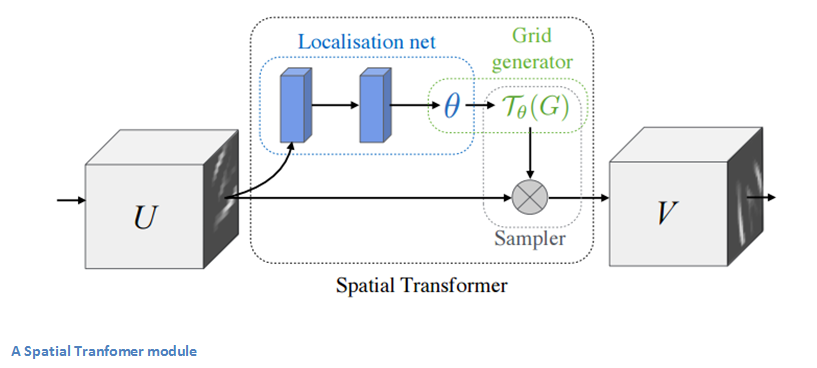
\includegraphics[scale=0.6]{SpatialTransformer}
  \caption{Spatial Transformer Networks.}
  \label{STN}
\end{figure}

Components: 

A localization network. Input: volume, Output: parameters of the spatial transformation that should be applied. The parameters can be 6 dimensional for an affine transformation.

The creation of a sampling grid that is the result of warping the regular grid with the affine transformation created in the localization network.

A sampler whose purpose is to perform a warping of the input feature map.

See description at \url{adeshpande3.github.io/The-9-Deep-Learning-Papers-You-Need-To-Know-About.html}
\eenum 
%\benum
% \subsection{Problems}
% \benum
% \item {\bf Why convolutions?}

% Vaguely related to \emph{symmetry}. See papers by Mallat, Bolcskei etc.  More precisely?

% Pooling loses information.  Need to take into account spatial information


%\eenum



\section{Recurrent neural networks (RNNs)}
\subsection{Setup}
\benum
\item \emph{Recurrent neural networks (RNNs)} are a class of models appropriate for sequential data. e.g., 

text, speech, video, DNA sequence, 

They exploit that the relation between temporal units is often invariant in time. Similar purpose as time series models in statistics. 

\item 

\emph{Input sequence} $x$, e.g., sentence:  

$$x = x^{<1>}, x^{<2>}, \ldots, x^{<t>}, \ldots, x^{<T_x>}$$

Has \emph{elements} $x^{<i>}$, e.g., words

\benum 
\item 
$x$ - "The cat is white"
\item  $x^{<1>}$ - "The"; $x^{<2>}$ - "cat"; $x^{<3>}$ - "is"; $x^{<4>}$ - "white"
\eenum 

\emph{Output sequence}, e.g., word labels: 

$$y = y^{<1>}, y^{<2>}, \ldots, y^{<t>}, \ldots, y^{<T_y>}$$
\benum 
\item  $y^{<1>}$ - pronoun; $y^{<2>}$ - noun; $y^{<3>}$ - verb; $y^{<4>}$ - adjective
\eenum 


(Do not need to have the same length)

%Recall training examples were $x^{(i)}$, so $x^{(i)<t>}$ is the $t$-th element of the $i$-th training example

\item \emph{Word representations}: use \emph{one-hot vectors} to represent words. Each element (word) will be a vector 

$$e_j = (0,\ldots, 0, 1, 0,\ldots, 0).$$ 

The length of the vector is the size of the \emph{dictionary}.

In principle, this reduces the problem to a supervised learning problem. However, the direct application of NNs is inefficient. Does not use sequential structure. 

\item RNN works sequentially: 

\benum 
\item 
Start with activations $a^{<0>}$, say 
$$a^{<0>}=0$$
\item 
At every step: construct activations $a^{<t>}$

Use previous activations $a^{<t-1>}$, and current input element $x^{<t>}$, to predict output element $y^{<t>}$. 

This prediction will be governed by parameters $W_{a}$, shared across time. 

\begin{align*}
a^{<t>} &= \sigma_1(W_{a}[a^{<t-1>},x^{<t>}]+b_a)\\
\hy^{<t>} &= \sigma_2(W_{y}a^{<t>}+b_y)
\end{align*}

As described by Andrej Karpathy "RNNs combine the input vector $x$ with their state vector $a$ with a fixed (but learned) function to produce a new state vector. This can in programming terms be interpreted as running a fixed program with certain inputs and some internal variables. Viewed this way, RNNs essentially describe programs."

\eenum 
\item Training: Backprop proceeds as before. 

Loss is often defined elementwise: $L(\hat y,y) = \sum_{t=1}^T \ell(\hat y^{<t>},y^{<t>})$


\item There are many variants: We saw \emph{Many-to-many} with equal input and output lengths. 

\emph{One-to-Many}: e.g., start with one input element, and produce entire sequence. eg., music generation. Feed each output element forward too $\hat y^{<t>}$

 See also Figure \ref{rnn}

\begin{figure}
  \centering
  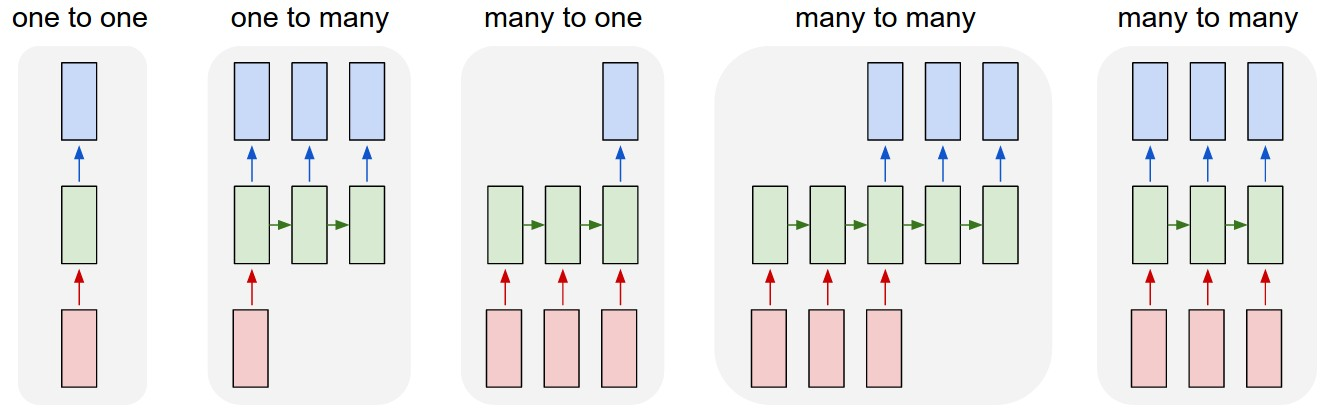
\includegraphics[scale=0.3]{diags.jpeg}
  \caption{RNNs.}
  \label{rnn}
\end{figure}


\item \emph{Gated Recurrent Unit (GRU)}: Can help better capture long-term dependence (Cho et al, 2014, Chung et al, 2014) 

Add \emph{memory cell} $c$, with elements $c^{<t>}$. This remembers the state.

e.g., which person is the current part of the sentence about?


Also add \emph{candidate update cell} $\tilde c^{<t>}$. This is the potential updated state. 

$$\tilde c^{<t>} = \tanh(W_c [c^{<t-1>},x^{<t>}]+b_c)$$

e.g., if the previous state is a name, and new word is a name, then candidate update is the new name

\emph{Gate}, or \emph{update gate}: determines whether or not there is an update (think 0, 1)

$$\Gamma_u = \sigma(W_u [c^{<t-1>},x^{<t>}]+b_u)$$

e.g., if previous state is a name, under what conditions should I switch topics? 

\benum 
\item John met Jane who was two years older. 
\item John met Jane but did not talk much.
\eenum 



\emph{Update rule}: 
$$c^{<t>} = \Gamma_u \odot \tilde c^{<t>} + (1-\Gamma_u) \odot c^{<t-1>}$$

Gate = 0, don't update. Gate = 1, update.

The entire GRU is a bit more complicated. Also includes \emph{relevance gate} $\Gamma_r$, tells us how relevant is $\tilde c$ to computing the next $c$ 

\begin{align*}
\tilde c^{<t>} &= \tanh(W_c [\Gamma_r  \odot c^{<t-1>},x^{<t>}]+b_c)\\
\Gamma_u &= \sigma(W_u [c^{<t-1>},x^{<t>}]+b_u)\\
\Gamma_r &= \sigma(W_r [c^{<t-1>},x^{<t>}]+b_r)\\
c^{<t>} & = \Gamma_u \odot \tilde c^{<t>} + (1-\Gamma_u) \odot c^{<t-1>}
\end{align*}


\item \emph{Long Short Term Memory (LSTM)} (Hochreiter, Schmidhuber, 1997): 

Similar, but more powerful (and more complicated). There is a separate \emph{forget gate} $\Gamma_f$, to control the update rule. There is a separate \emph{output gate}  $\Gamma_o$, to control output. 

\begin{align*}
\tilde c^{<t>} &= \tanh(W_c [a^{<t-1>},x^{<t>}]+b_c)\\
\Gamma_u &= \sigma(W_u [a^{<t-1>},x^{<t>}]+b_u)\\
\Gamma_f &= \sigma(W_f [a^{<t-1>},x^{<t>}]+b_f)\\
\Gamma_o &= \sigma(W_o [a^{<t-1>},x^{<t>}]+b_o)\\
c^{<t>} & = \Gamma_u \odot \tilde c^{<t>} + \Gamma_f \odot c^{<t-1>}\\
a^{<t>} & = \Gamma_o \odot \tanh(c^{<t>})
\end{align*}

See Figure \ref{lstm}. 

\begin{figure}
  \centering
  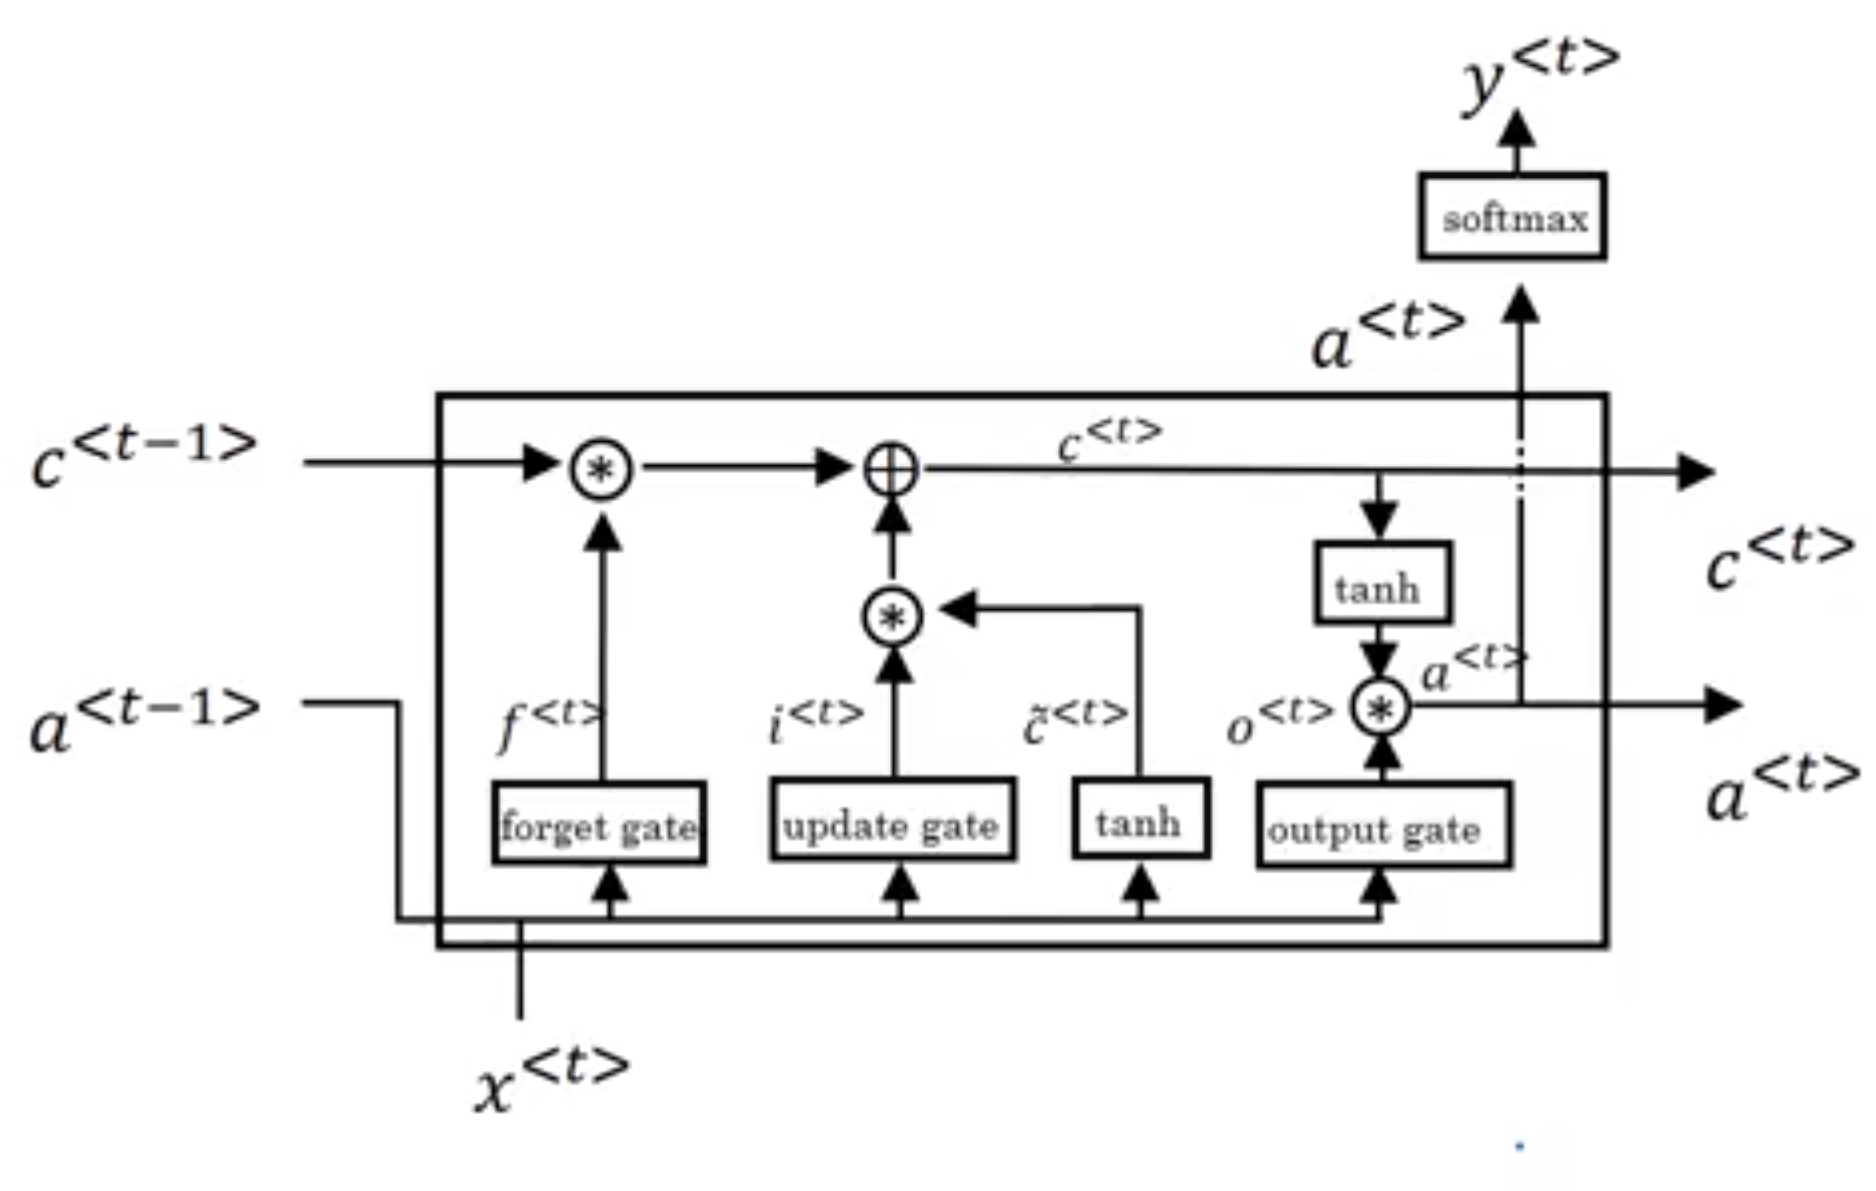
\includegraphics[scale=0.3]{lstm.png}
    \caption{LSTM. Courtesy of Andrew Ng's course.}
    \label{lstm}
\end{figure}


\item  Karpathy: "An important point to realize is that even if your inputs/outputs are fixed vectors, it is still possible to use this powerful formalism to process them in a sequential manner. For instance, [we can] learn a recurrent network policy that steers its attention around an image; In particular, learn to read out house numbers from left to right (Ba et al. 2014, Multiple Object Recognition with Visual Attention)."

\item Attention model. Bahdanau et al, Neural Machine Translation by Jointly Learning to Align and Translate (2014): Figure \ref{attn}

See \url{https://lilianweng.github.io/lil-log/2018/06/24/attention-attention.html} for a detailed description


\begin{figure}
  \centering
  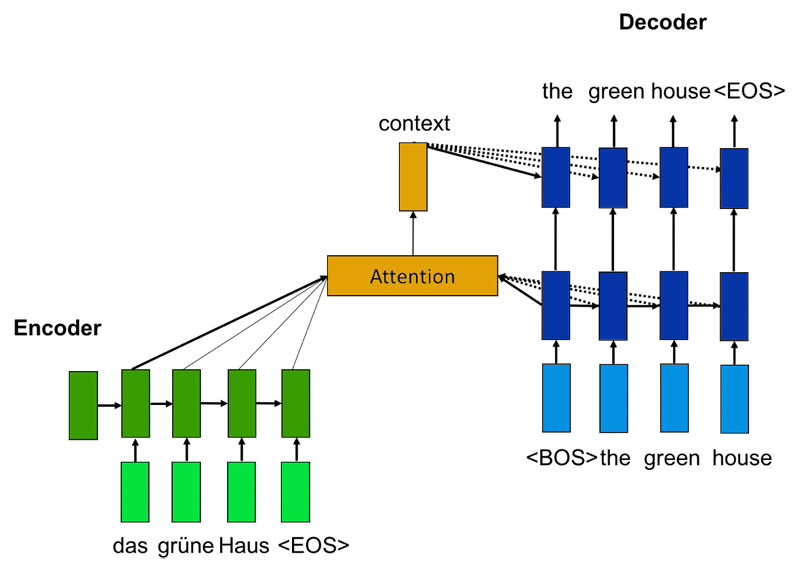
\includegraphics[scale=0.3]{attn}
    \caption{Attention Model.}
    \label{attn}
\end{figure}


\item Some applications: 

Captioning: Figure \ref{c}

\begin{figure}
  \centering
  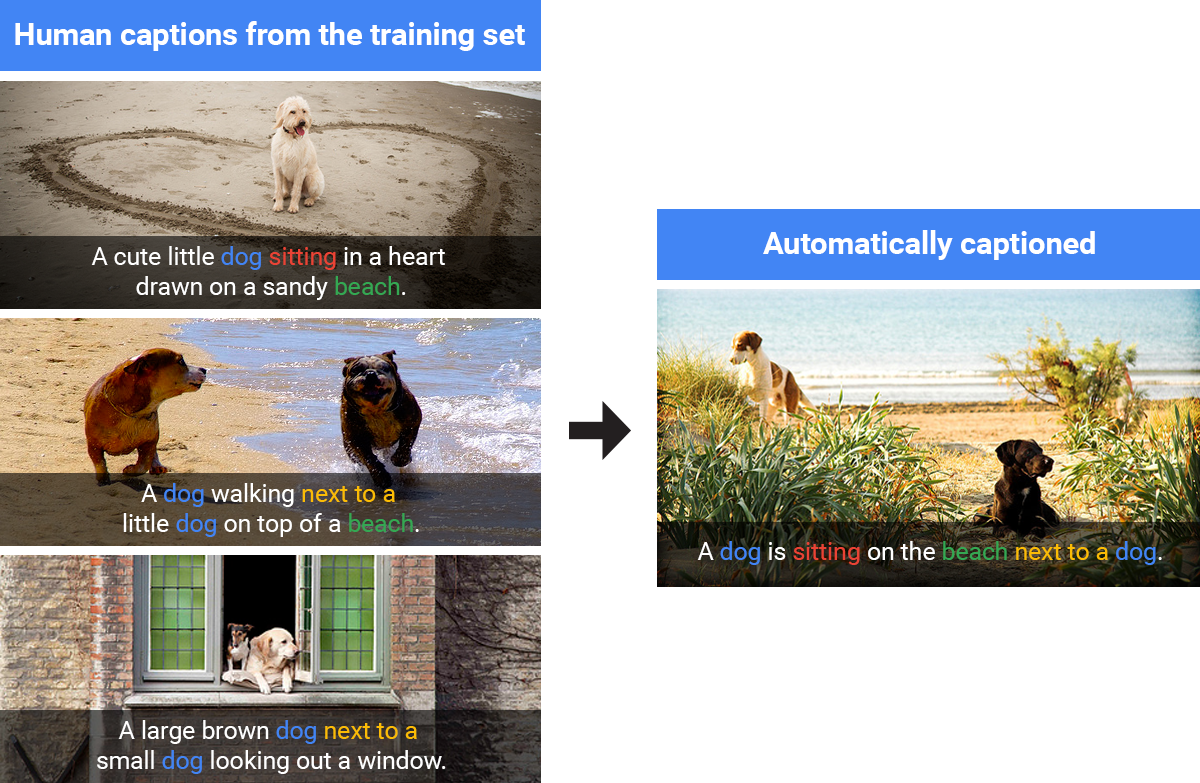
\includegraphics[scale=0.4]{Caption4.png}
    \caption{Captioning,  Google Brain, 2016. Show and Tell: Lessons learned from the 2015 MSCOCO Image Captioning Challenge. \url{https://ai.googleblog.com/2016/09/show-and-tell-image-captioning-open.html}}
    \label{c}
\end{figure}

Text generation: (Pretty bad, example from Karpathy's blog): "Naturalism and decision for the majority of Arab countries' capitalide was grounded
by the Irish language by [[John Clair]], [[An Imperial Japanese Revolt]], associated  with Guangzham's sovereignty. His generals were the powerful ruler of the Portugal 
in the [[Protestant Immineners]], which could be said to be directly in Cantonese 
Communication, which followed a ceremony and set inspired prison, training.

\item Interestingly, some sequence problems can be addressed well with convolutional networks. e.g., 

Yoon Kim - Convolutional Neural Networks for Sentence Classification - EMNLP - 2014

WaveNet by Google for sound synthesis uses an "atrous convolution", which is a hierarchical structure. (Fig. \ref{wavenet})

\begin{figure}
  \centering
  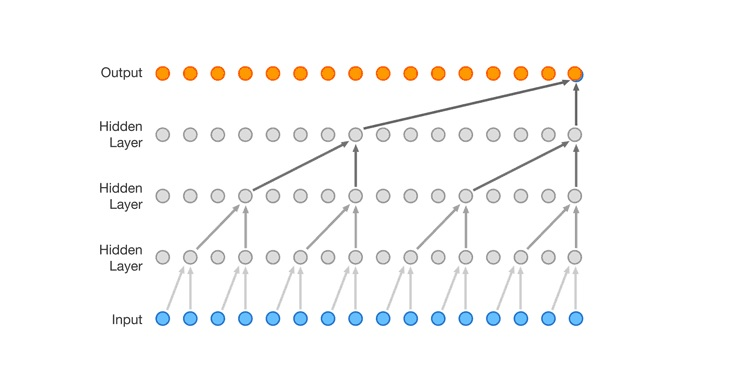
\includegraphics[scale=0.8]{wavenet.jpg}
    \caption{Wavenet.}
    \label{wavenet}
\end{figure}



\item See also \url{http://colah.github.io/posts/2014-07-NLP-RNNs-Representations/}

\url{http://colah.github.io/posts/2015-08-Understanding-LSTMs/}

Excellent description: \url{http://karpathy.github.io/2015/05/21/rnn-effectiveness/}

\eenum 

\subsection{Sequence Learning}

%------------------------------------------------
\subsubsection{Motivation} % Sections can be created in order to organize your presentation into discrete blocks, all sections and subsections are automatically printed in the table of contents as an overview of the talk
%------------------------------------------------
\benum
\item 
 {Examples of problems involving sequence data}
\begin{itemize}
\item Speech recognition
\item Music generation
\item Time series forecasting
\item Machine translation
\item Conversation agents
\item Image captioning
\end{itemize}
 

\item 
 {Limitations of feedforward networks}

Recall the structure of a basic feedforward network:  Figure \ref{MLP}
\begin{figure}
  \centering
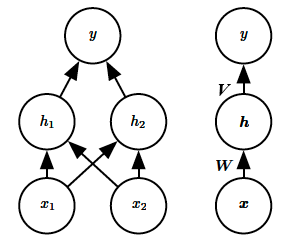
\includegraphics[width=0.4\linewidth]{mlp.png}
    \caption{MLP.}
    \label{MLP}
\end{figure}

\begin{align*}
h &= \sigma_1(b+Wx)\\
o &= c+Vh\\
\hat{y} &= \text{softmax}(o)
\end{align*}
Problem: How to learn from a sequence of inputs $x_1, x_2,\dots,x_\tau$?
%Want to allow our sequence of inputs and outputs to vary in length for different examples. 

%Want to learn dependencies across a (potentially long) input sequence.
 

\item 
 {Sequence Models}.  Figure \ref{rnn-types}

\begin{figure}
  \centering
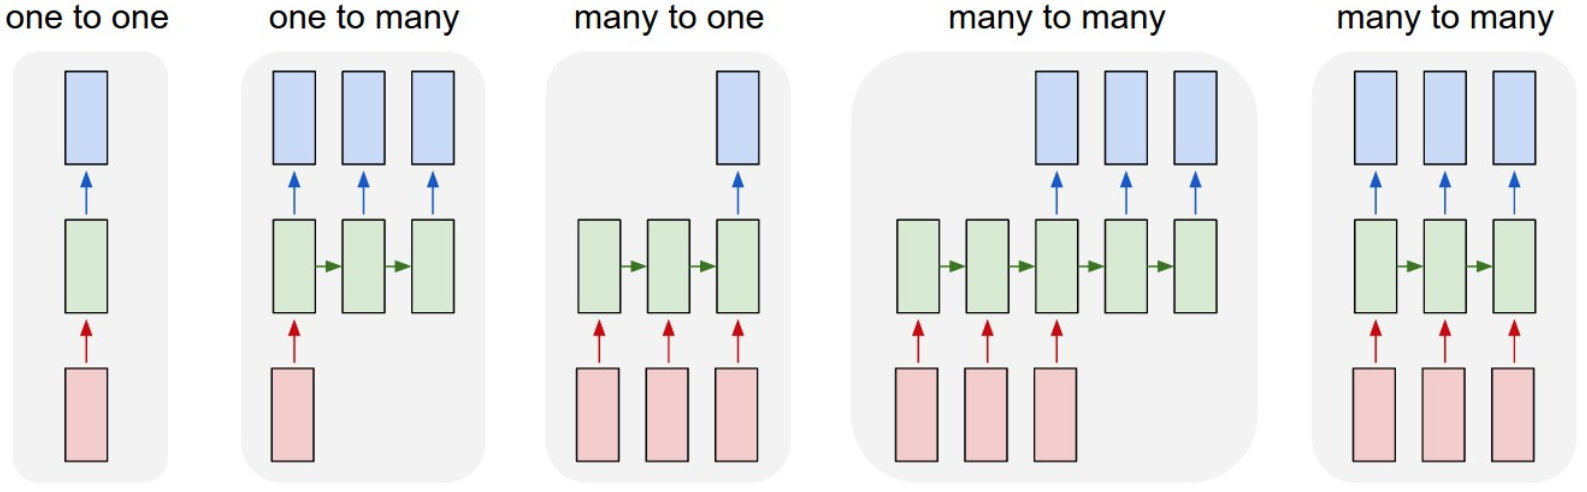
\includegraphics[width=0.9\linewidth]{rnn-types.png}
    \caption{RNN types.}
    \label{rnn-types}
\end{figure}
We will focus on the many-to-many cases. Requirements:
\begin{enumerate}
\item Output $\hat{y}_t$ should depend on the sequence so far, $x_1,\dots,x_t$.
\item We may not know the length of a particular input sequence ahead of time.
\end{enumerate}
\eenum

\subsection{Sequence Models}
\subsubsection{RNNs} % A subsection can be created just before a set of slides with a common theme to further break down your presentation into chunks
\benum
\item 
 {A Simple Recurrent Neural Network}.  Figure \ref{Simple RNN}

\begin{figure}
  \centering
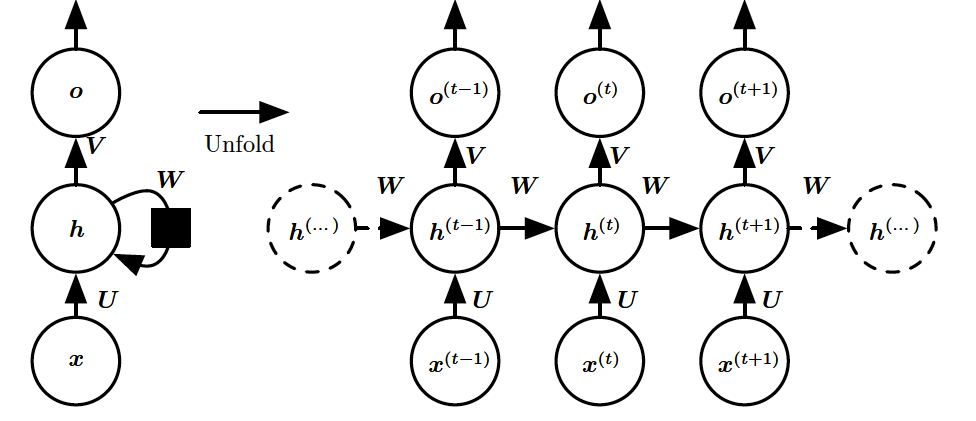
\includegraphics[width=0.8\linewidth]{rnn.png}
    \caption{Simple RNN.}
    \label{Simple RNN}
\end{figure}

\begin{align*}
h_t &= \sigma_1(b+Wh_{t-1}+Ux_t)\\
o_t &= c+Vh_t\\
\hat{y}_t &= \text{softmax}(o_t)
\end{align*}
 

\item 
 {A Simple Recurrent Neural Network}

RNNs allow us to learn a single model, rather than a separate one for each time step.
\begin{enumerate}
\item The model is specified in terms of \textit{transitions} from one state $h_t$ to the next.
\item Parameters are shared across time.
 
\end{enumerate}
Loss function is a sum of losses at each time step $t$:
$$L(\hat{y},y)=\sum_{t=1}^T \ell(\hat{y}_t, y_t)$$
 

\item 
 {Training RNNs}

Training proceeds as before using \textbf{backpropagation through time} on the unrolled computation graph.
 
We cannot easily parallelize training since each step is dependent on the one before it.
 
\textbf{Teacher forcing} can be used when there are output-to-hidden recurrent connections. Ground truth is fed to the model instead of its own output.  Figure \ref{Teacher forcing}
\begin{figure}
\centering
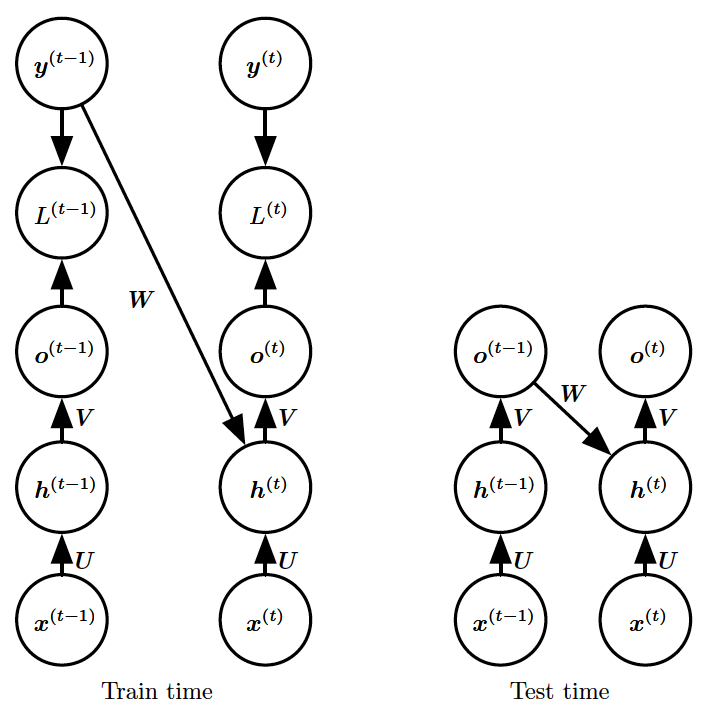
\includegraphics[height=0.5\linewidth]{teacher-forcing.png}
    \caption{Teacher forcing.}
    \label{Teacher forcing}
\end{figure}
 

\item 
 {Modeling Joint Probability Distributions}

When we use a negative log-likelihood training objective,
$$\ell(\hat{y}_t,y_t) = -\log{\Pr(y_t\,|\,x_1,\dots,x_t)}$$
we train the RNN to estimate the conditional distribution of the next sequence element $y_t$ given the past inputs.
 
We typically use the softmax function as the output layer to obtain normalized probabilities for each class.
$$\text{softmax}(o)_i=\frac{e^{o_i}}{\sum_{j=1}^\tau e^{o_j}}$$
 

RNNs can model arbitrary probability distributions of some sequence $y$ over another sequence $x$.
$$\Pr(y_1,\dots,y_\tau\,|\,x_1,\dots,x_\tau) = \prod_{t=1}^\tau \Pr(y_t\,|\,x_1,\dots,x_t)$$
To remove the conditional independence assumption, we can add output-to-hidden connections.
$$\Pr(y_1,\dots,y_\tau\,|\,x_1,\dots,x_\tau) = \prod_{t=1}^\tau \Pr(y_t\,|\,y_1,\dots,y_{t-1}, x_1,\dots,x_t)$$
 

Some challenges:
\begin{enumerate}
\item What if we want a given output $y_t$ to depend on the entire sequence $x_1,\dots,x_\tau$?
\item How do we map a sequence $x$ to a sequence $y$ when they can differ in length from each other?
\end{enumerate}
\vspace{5mm}
We will see the solutions later in the context of machine translation.
 
First, a fundamental problem: \begin{center}\textcolor{red}{RNNs have trouble learning long-term dependencies.}\end{center}
 \eenum

\subsubsection{Training Challenges}
\benum
\item 
 {Learning Long-Term Dependencies}

%The gap between relevant information and when it is needed may be large.
%e.g. predicting the last word in ``I grew up in France... I speak fluent \textit{French}." 
Sentence 1: ``Jane walked into the room. John walked in too. Jane said hi to...'' 

Sentence 2: ``Jane walked into the room. John walked in too. It was late in the day, and everyone was walking home after a long day at work. Jane said hi to...'' 

\begin{center}
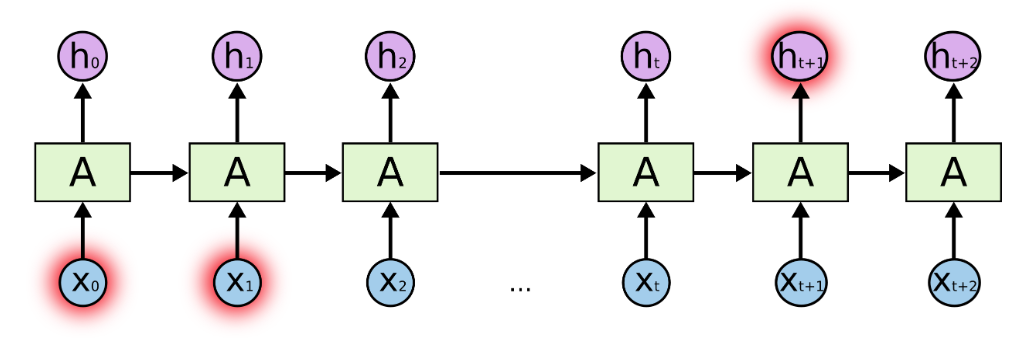
\includegraphics[height=0.25\linewidth]{rnn-long-term.png} 
\end{center}

RNNs have trouble learning dependencies from inputs with a large time difference from the predicted output.
 

% Each term in the sum is the contribution of the weight matrix at time k to the error at time t. When this term becomes very small, then the contribution of the inputs at time k to the value of the hidden state at time t becomes small.
\item 
 {Vanishing or Exploding Gradients}

Suppose we have an RNN with state $h_t$, input $x_t$, and cost $\mathcal{E}$.\footnote{The original paper uses this formulation instead of $h_t=\sigma(Wh_{t-1}+Ux_t+b)$ and says they are equivalent.}
$$h_t = W\sigma(h_{t-1})+Ux_t+b$$
$$\mathcal{E}=\sum_{1\leq t\leq \tau}\mathcal{E}_t,\quad \mathcal{E}_t=\mathcal{L}(h_t)$$
Let's calculate the gradient over one input sequence.
\begin{align*}
\frac{\partial\mathcal{E}}{\partial W} &= \sum_{1\leq t\leq\tau} \frac{\partial\mathcal{E}_t}{\partial W}\\
\frac{\partial\mathcal{E}_t}{\partial W} &= \sum_{1\leq k \leq t} \left(\frac{\partial\mathcal{E}_t}{\partial h_t}\frac{\partial h_t}{\partial h_k}\frac{\partial^+h_k}{\partial W}\right)\\
\frac{\partial h_t}{\partial h_k} &= \prod_{t\geq i>k}\frac{\partial h_i}{\partial h_{i-1}}=\prod_{t\geq i>k} {W}^\top\,\text{diag}(\sigma^\prime(h_{i-1}))
\end{align*}
 

\item 
 {Vanishing or Exploding Gradients}

The cause is the Jacobian matrix $J$. We have a product of $t-k$ Jacobians.

\begin{align*}
J&=\frac{\partial h_{k+1}}{\partial h_k}=W^\top\text{diag}(\sigma^\prime(h_k))\\
\|J\|&=\left\|\frac{\partial h_{k+1}}{\partial h_k}\right\|\leq\underbrace{\left\|W^\top\right\|}_{\lambda_1}\;\underbrace{\left\|\text{diag}(\sigma^\prime(h_k))\right\|}_{\gamma}=\lambda_1\gamma
\end{align*}

$\lambda_1$ is the largest singular value of $W$. $\gamma=1$ for tanh and $\gamma=\frac{1}{4}$ for sigmoid.
$$\left\|\prod_{i=k}^{t-1}\frac{\partial h_{i+1}}{\partial h_i}\right\| \leq (\lambda_1\gamma)^{t-k}$$
When $t \gg k$:
\begin{itemize}
\item
If $\lambda_1<\frac{1}{\gamma}$, the gradients \textit{will} vanish.
\item
If $\lambda_1>\frac{1}{\gamma}$, the gradients \textit{may} explode.
\end{itemize}
 

\item 
 {How to deal with gradient problems?}

\begin{enumerate}
\item Modify the training algorithm: \textbf{gradient clipping}.
\begin{itemize}
\item Commonly used when training all variants of RNNs.
\end{itemize}
\item Use a different activation function: \textbf{ReLUs}.
\begin{itemize}
\item Primarily used for deep neural nets (e.g. computer vision).
\end{itemize}
\item Use a more complex neural architecture: \textbf{LSTMs and GRUs}.
\end{enumerate}
 

\item 
 {Gradient Clipping}. Figure \ref{Gradient Clipping}

\begin{figure}
\centering
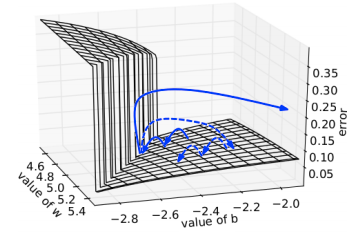
\includegraphics[height=0.35\linewidth]{gradient-clip2.png}
    \caption{Gradient Clipping.}
    \label{Gradient Clipping}
\end{figure}

Addresses the problem of exploding gradients by preventing parameter updates from being too large.\\
\begin{algorithmic}
\State {$g \leftarrow \frac{\partial\mathcal{E}}{\partial\theta}$}
\If{$\|g\|\geq$ threshold}
    \State{$g \leftarrow \frac{\text{threshold}}{\|g\|}g$}
\EndIf
%\If{hi}{}
\end{algorithmic}
Does gradient clipping affect convergence?
 

\item 
 {ReLU}.  Figure \ref{ReLU}
\begin{figure}
\centering
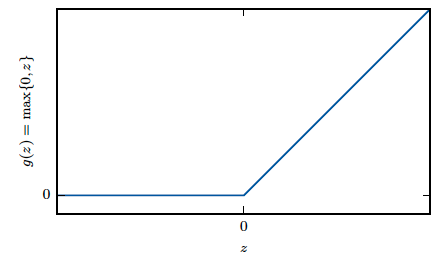
\includegraphics[height=0.3\linewidth]{relu.png}
    \caption{ReLU.}
    \label{ReLU}
%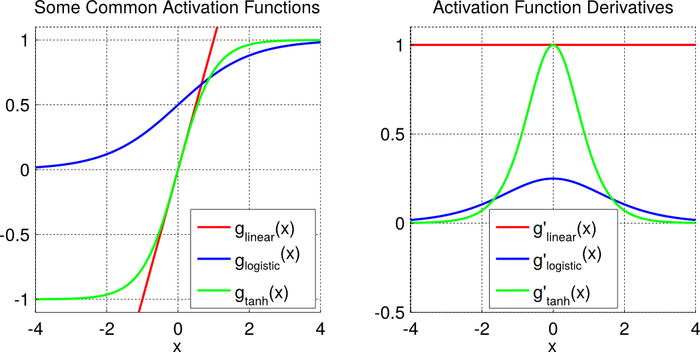
\includegraphics[height=0.3\linewidth]{activation.png}
\end{figure}

Since the derivative is 1 when $z>0$, gradients flow more easily compared to sigmoid or tanh units. Also computationally efficient.  

Can lead to ``dead neurons'' during training. Is this a problem? 

Empirically, ReLU has been shown to be very effective.

%(as long as some of the hidden units in each layer remain alive).
 \eenum

\subsubsection{LSTM and GRU}
\benum
\item 
 {New Recurrent Architectures}

We will introduce the Long Short-Term Memory (LSTM) and Gated Recurrent Unit (GRU) architectures. 
\begin{itemize}
\item Address the problem of vanishing gradients.
\item Considered the state of the art for many deep learning tasks.
\begin{itemize}
\item Image captioning, parsing, speech recognition, machine translation, reinforcement learning
\end{itemize}
\end{itemize}
 

\item 
 {Long Short-Term Memory Network (Hochreiter 1997)}.  Figure \ref{LSTM}

\begin{figure}
\centering
% 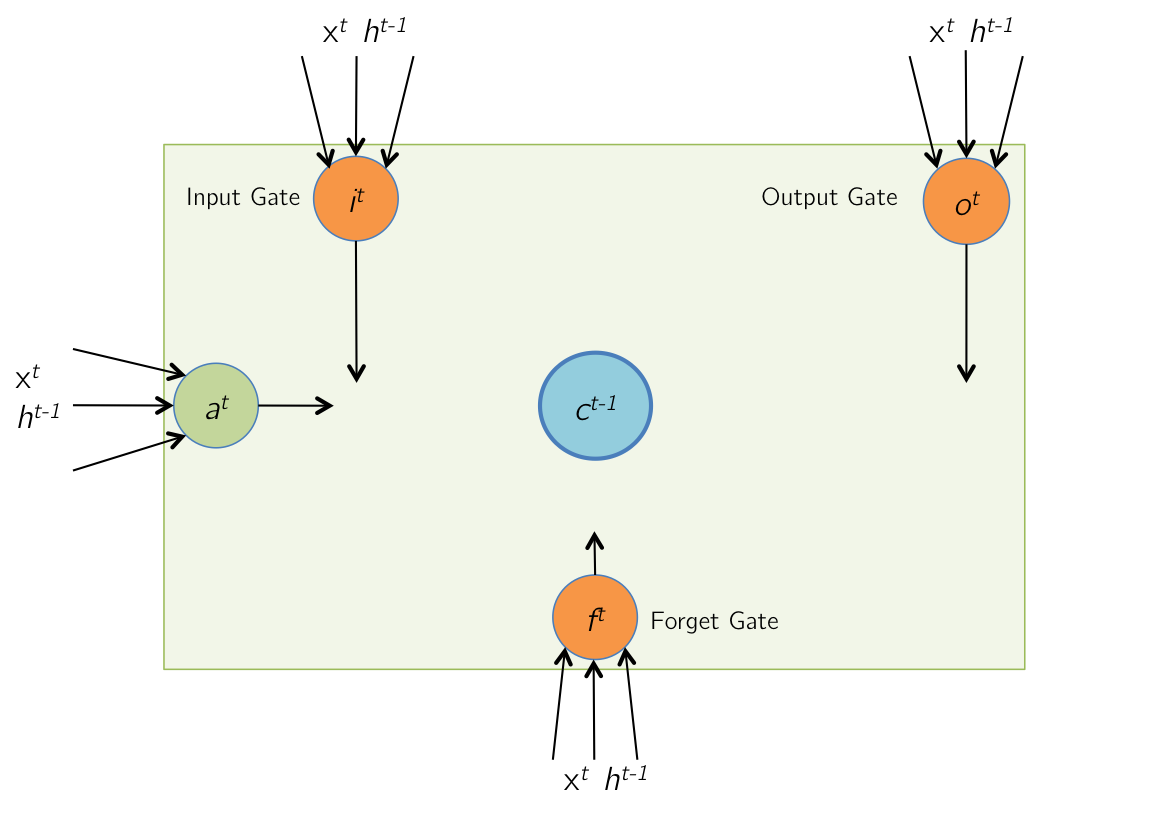
\includegraphics[height=0.25\linewidth]{lstm1.png}
% 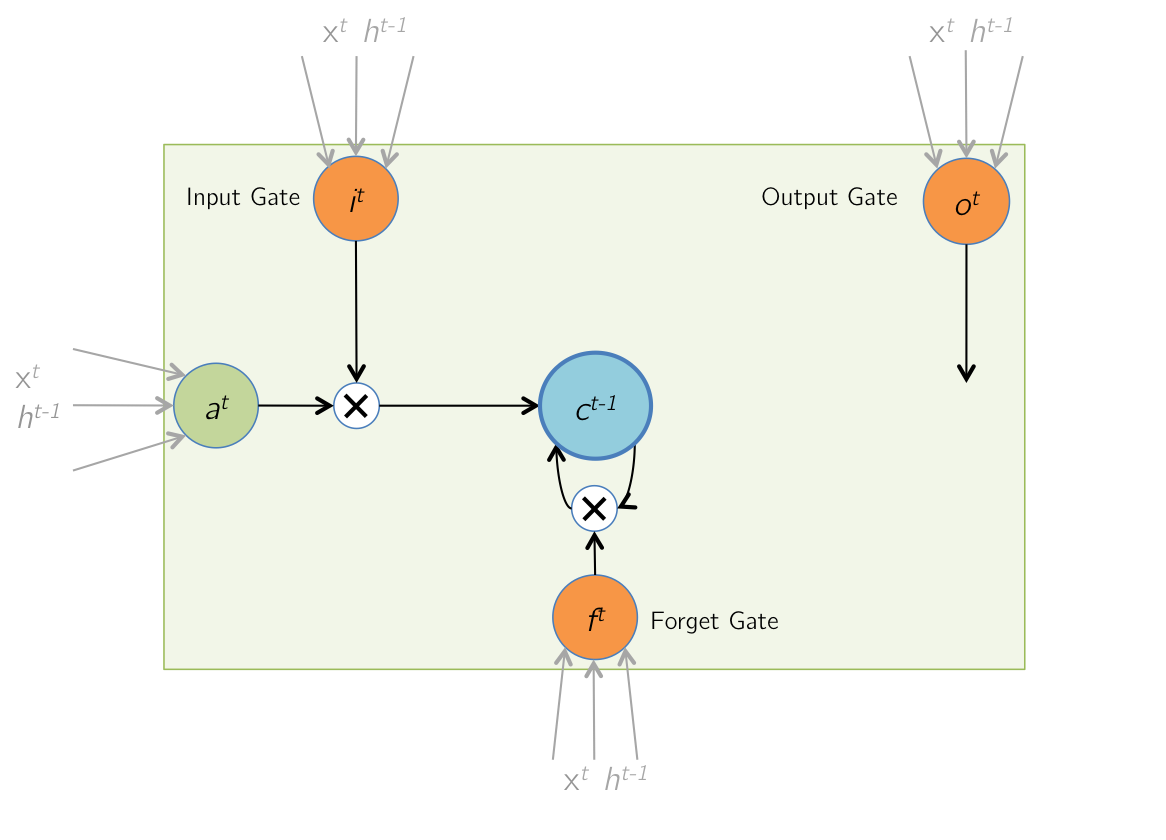
\includegraphics[height=0.25\linewidth]{lstm2.png}
% 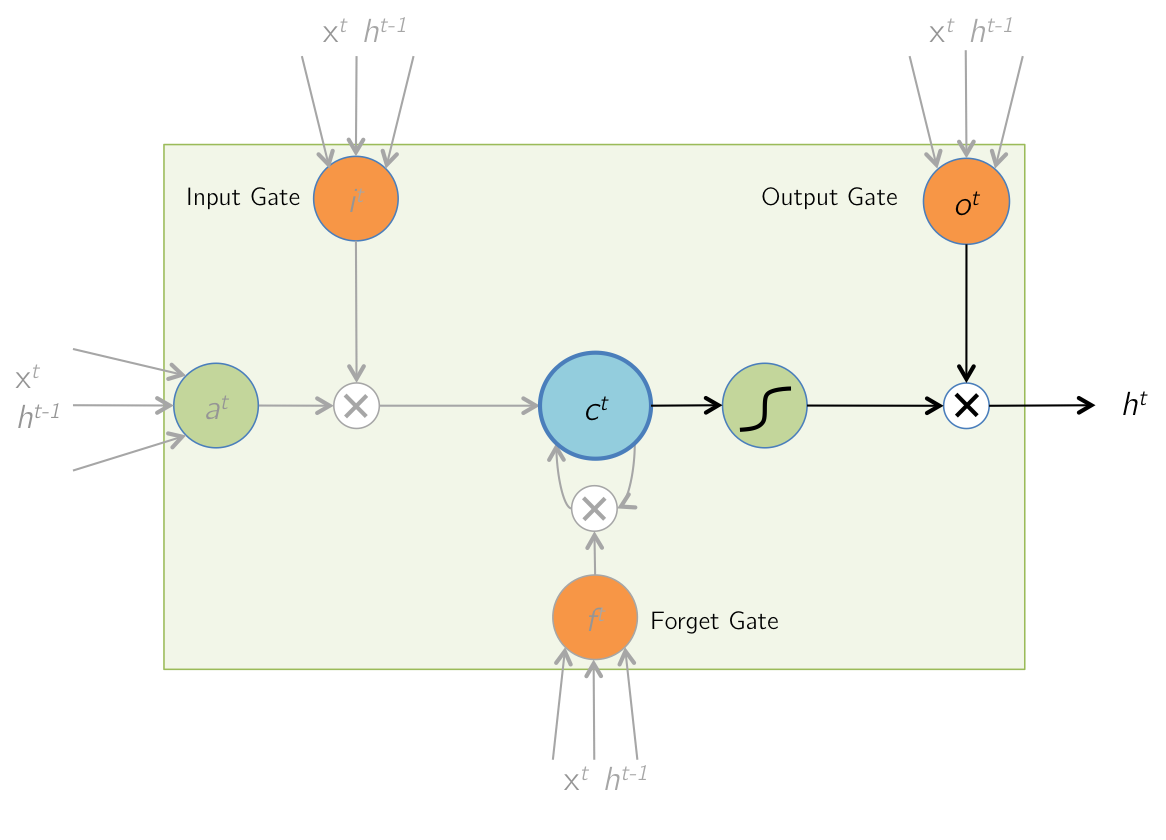
\includegraphics[height=0.25\linewidth]{lstm3.png}
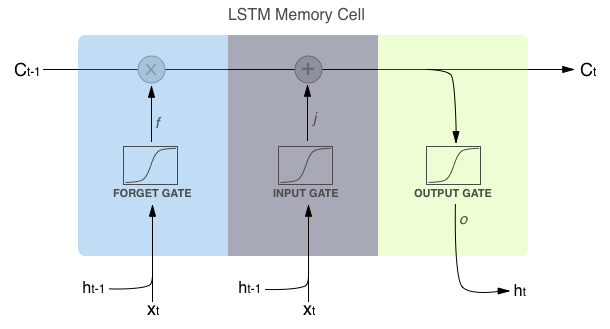
\includegraphics[height=0.33\linewidth]{lstm-cell.png}
    \caption{LSTM.}
    \label{LSTM}
\end{figure}

\begin{align*}
% f^{(t)} &= \sigma_g(W_fx^{(t)}+U_fh^{(t-1)}+b_f)\\
% i^{(t)} &= \sigma_g(W_ix^{(t)}+U_ih^{(t-1)}+b_i)\\
% o^{(t)} &= \sigma_g(W_ox^{(t)}+U_oh^{(t-1)}+b_o)\\
% a^{(t)} &= \sigma_t(W_cx^{(t)}+U_ch^{(t-1)}+b_c)\\
% c^{(t)} &= i^{(t)}\odot a^{(t)} +f^{(t)}\odot c^{(t-1)}\\
% h^{(t)} &= o^{(t)}\odot \sigma_t(c^{(t)})
f_t &= \sigma_g(W_fx_t+U_fh_{t-1}+b_f)\\
i_t &= \sigma_g(W_ix_t+U_ih_{t-1}+b_i)\\
o_t &= \sigma_g(W_ox_t+U_oh_{t-1}+b_o)\\
a_t &= \sigma_t(W_cx_t+U_ch_{t-1}+b_c)\\
c_t &= i_t\odot a_t +f_t\odot c_{t-1}\\
h_t &= o_t\odot \sigma_t(c_t)
\end{align*}
 

\item 
 {LSTM and Backpropagating Gradients}

Recall the equation to update the cell state:
$$c_t = i_t\odot a_t +f_t\odot c_{t-1}$$
The original LSTM did not have a forget gate, allowing error to flow unchanged from $c_t$ to $c_{t-1}$.
\begin{itemize}
\item Referred to as the constant error carousel.
\end{itemize}
With a forget gate, if $f_t\approx 1$, we achieve the same effect.
\begin{itemize}
\item Can initialize the forget gate bias to $1$ before training.
\end{itemize}
%http://harinisuresh.com/2016/10/09/lstms/
 

\item 
 {Gated Recurrent Unit (Cho et. al 2014)}


\begin{align*}
u_t &= \sigma(W_ux_t+U_uh_{t-1}+b_u)\\
r_t &= \sigma(W_rx_t+U_rh_{t-1}+b_r)\\
a_t &= \sigma_t(W_ix_t+r_t\odot U_ih_{t-1}+b_i)\\
h_t &= u_t\odot h_{t-1} + (1-u_t)\odot a_t
\end{align*}
Hidden units that learn to capture...
\begin{itemize}
\item short-term dependencies will tend to have reset gates that are frequently active. 
\item longer-term dependencies will have update gates that are mostly active.
\end{itemize}
Takeaway: Similar performance to LSTM, but fewer parameters.
 \eenum
 

\subsection{Machine Translation}
\benum
\item 
 {Neural Machine Translation in 2016}.  Figure \ref{Neural Machine Translation in 2016}

\begin{figure}
\centering
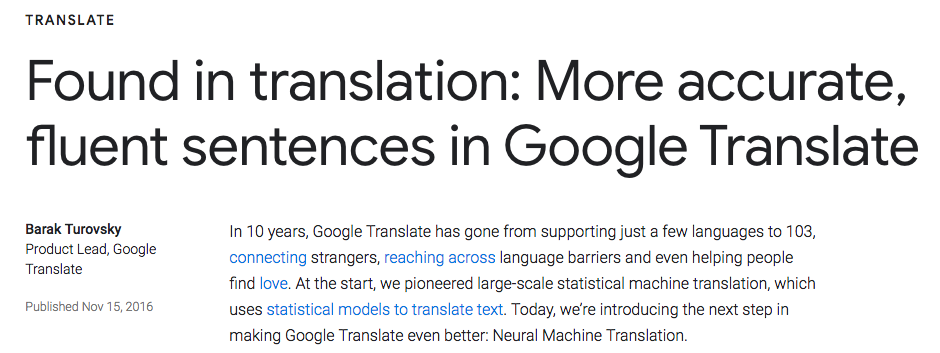
\includegraphics[height=0.3\linewidth]{gt1.png}
\vspace{5mm}
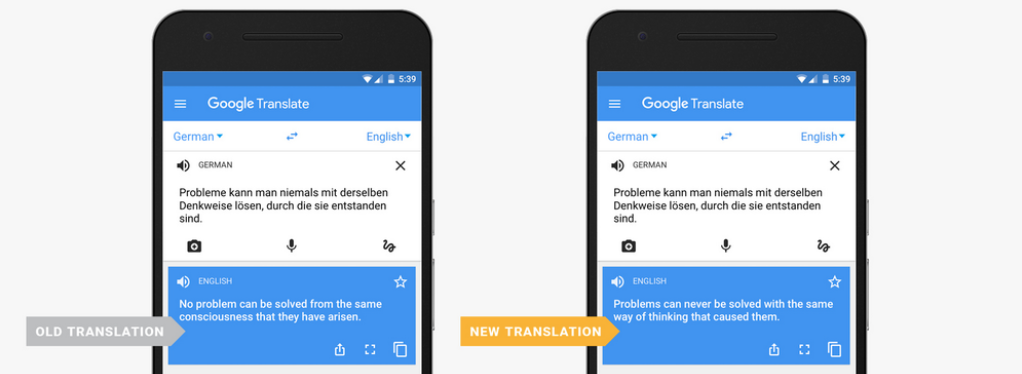
\includegraphics[height=0.3\linewidth]{gt2.png}
    \caption{Neural Machine Translation in 2016.}
    \label{Neural Machine Translation in 2016}
\end{figure}
 
\item 
 {History}

A bilingual translation task:

``The cat sat on the mat." $\rightarrow$ ``Le chat s'est assis sur le tapis."
$$***$$
2003: Neural language model introduced by Bengio et al. This was incorporated into existing phrase-based statistical machine translation (SMT) systems.

2014: Encoder-decoder RNN introduced by Cho et. al for use in SMT.

2015: Attention model proposed by Bahdanu et. al for end-to-end neural machine translation (NMT).

2017: Transformer model proposed by Vaswani et. al. This is the current state-of-the-art.
 

\item 
 {Word Representations}

How should the model encode a word token in a sequence?
 
Attempt 1: One-hot vectors. Represent every word as an $\mathbb{R}^{|V|\times 1}$ vector with all zero's except for a single one depending on the index of the word in the vocabulary $V$.
\begin{itemize}
\item $e(\text{cat})=\left[\begin{smallmatrix}
0 & 0 & 0 & \dots & 1 & \dots & 0
\end{smallmatrix}\right]^\top$
\item Does not capture semantic similarity between words!
\item Scales poorly with size of vocabulary.
\end{itemize}
 

\item 
 {Word Representations}

Attempt 2: Word embeddings. Model each word in a low-dimensional continuous space with dimension $M$.
\begin{itemize}
\item $e(\text{cat})=\left[\begin{smallmatrix}
0.1 & 0.33 & 0.72 & \dots & 0.59
\end{smallmatrix}\right]^\top$
\item Intuition: ``A word is defined by the company it keeps.''
\end{itemize}
\vspace{5mm}
Has revolutionized natural language processing (NLP) tasks since 2010.
\begin{itemize}
\item Popular word embeddings: word2vec, GloVe, ELMo
\end{itemize}
 

\item 
 {Encoder-Decoder Model}

How to map an input sequence to an output sequence where the lengths are not necessarily the same?
 
\textbf{Encoder} RNN processes the input sequence and emits a context vector $c$, which is the model's final hidden state, $h_{\tau_x}$.
$$h_t = f(h_{t-1},e(x_t))$$

\textbf{Decoder} RNN generates the output sequence based on $c$ and the previous output.
\begin{align*}
s_t &= f(s_{t-1}, e(y_{t-1}), c)\\
\Pr(y_t) &= g(s_t, e(y_{t-1}), c)
\end{align*}
Jointly trained to maximize $\log{\Pr_\theta(y_1,\dots,y_{\tau_y}\,|\,x_1,\dots,x_{\tau_x})}$.
% \begin{figure}
% 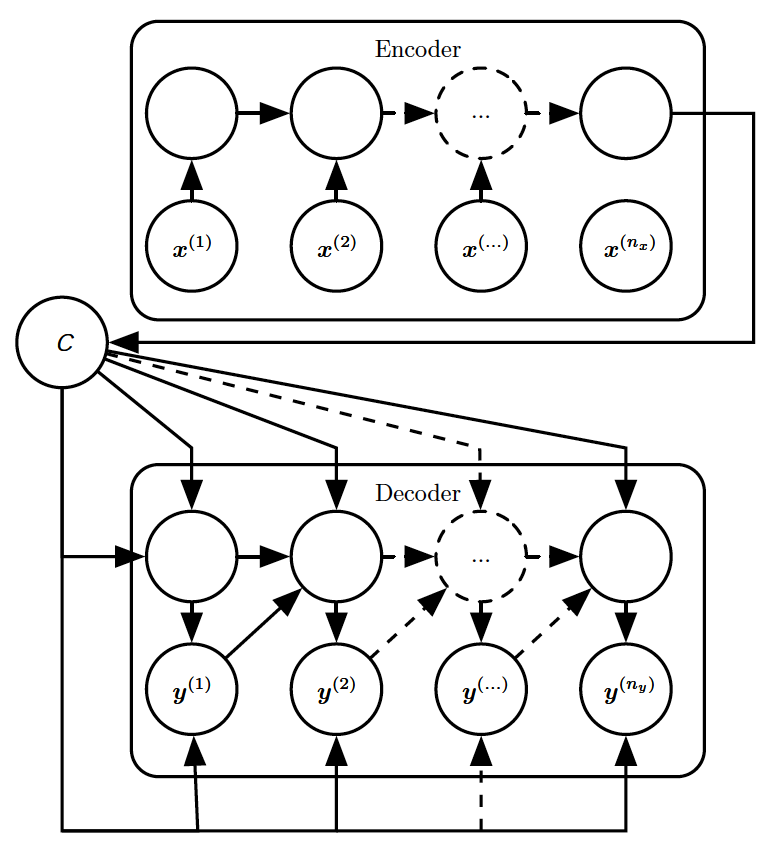
\includegraphics[height=0.3\linewidth]{encdec.png}
% \end{figure}
 

\item  Figure \ref{Encoder-Decoder Model}

Task: English-to-French translation.

Training data: 348M sentences from Europarl, news commentary, etc.

Test data: 3000 sentences from a standard newstest dataset.
\begin{figure}
\centering
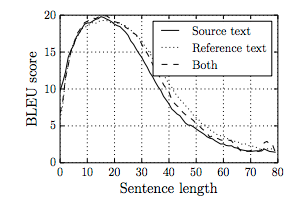
\includegraphics[height=0.3\linewidth]{encdec-smt1.png}
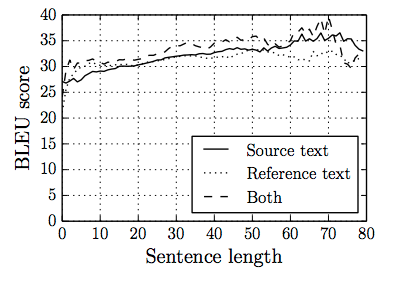
\includegraphics[height=0.3\linewidth]{encdec-smt2.png}
\caption{Translation quality vs. sentence length. RNN left, SMT right.}
\label{Encoder-Decoder Model}
\end{figure}

 

\item   Figure \ref{Sample-rnn}

\begin{figure}
\centering
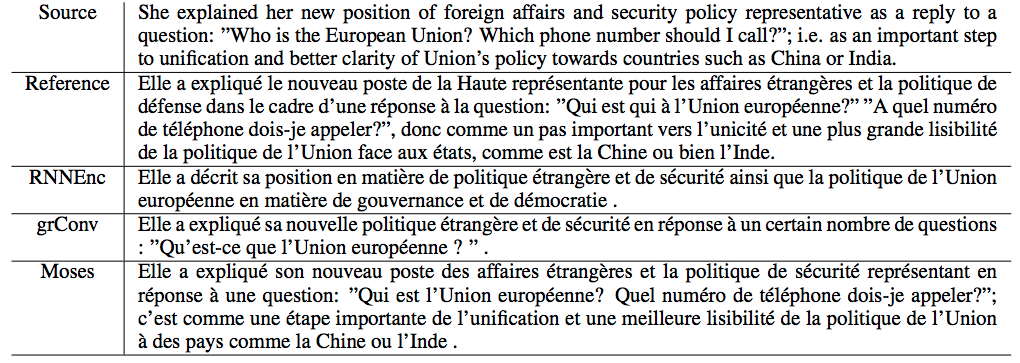
\includegraphics[height=0.35\linewidth]{sample-sents.png}
\caption{Sample output of two RNN models compared to the SMT system, Moses.}
\label{Sample-rnn}
\end{figure}
Problem: the neural network must compress all information in the source sentence into a single, fixed-length vector.
 \eenum

\subsubsection{Attention}
\benum
\item 
 {Encoder-Decoder Model with Attention}

Decoder RNN is similar to before, but each context vector $c_t$ is distinct for each target word $y_t$:
\begin{align*}
s_t &= f(s_{t-1}, e(y_{t-1}), c_t)\\
\Pr(y_t) &= g(s_t, e(y_{t-1}), c_t)
\end{align*}
$c_t$ is a weighted sum of \textit{annotations} $h_1,\dots,h_{\tau_x}$ to which the encoder maps the input sentence.
$$c_t = \sum_{j=1}^{\tau_x} \alpha_{tj}h_j$$
How are $\alpha$ and $h$ computed?
 

\item 
The encoder is a ``\textbf{bidirectional RNN}."
 
Forward RNN reads the input as ordered and computes a sequence of forward hidden states $\overrightarrow{h}_1,\dots,\overrightarrow{h}_{\tau_x}$.
 
Backward RNN reads the input in reverse and computes a sequence of backward hidden states $\overleftarrow{h}_1,\dots,\overleftarrow{h}_{\tau_x}$.
 
An annotation for a word $x_j$ is the concatenation of the two hidden states.
$$h_j=\left[\overrightarrow{h}_j, \overleftarrow{h}_j\right]$$
Due to the tendency of RNNs to better represent recent inputs, the annotation $h_j$ will be focused on the words around $x_j$.
 

\item 
 {Encoder-Decoder Model with Attention}.  Figure \ref{Attention}

\begin{figure}
\centering
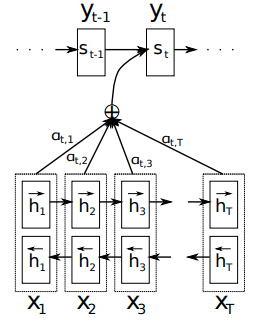
\includegraphics[height=0.35\linewidth]{attention.png}
\caption{Attention}
\label{Attention}
\end{figure}
To compute the weight $\alpha_{ij}$ of each annotation $h_j$, we use an \textbf{alignment model}. This is just a single-layer feedforward NN.
\begin{align*}
e_{ij} &= a(s_{i-1}, h_j)\\
\alpha_{ij} &= \text{softmax}(e_{ij})
\end{align*}
The alignment model scores how well the inputs around position $j$ and the output at position $i$ match.

It is interesting that the alignment refers to representations that are learned from the data. Namely, the annotations $h_j$ and the Decoder states $s_t$

\item   Figure \ref{Encoder-Decoder Model with Attention}

Same training and test data as before (English-to-French).

\begin{figure}
\centering
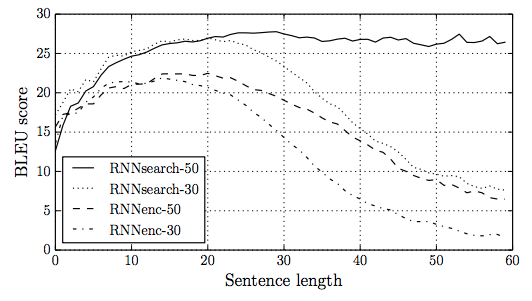
\includegraphics[height=0.4\linewidth]{attention-encdec.png}
    \caption{Encoder-Decoder Model with Attention.}
    \label{Encoder-Decoder Model with Attention}
\end{figure}

The encoder-decoder model with attention does much better on longer sentences.
 

\item  Figure \ref{A sample alignment found by RNNsearch-50}


\begin{figure}
\centering
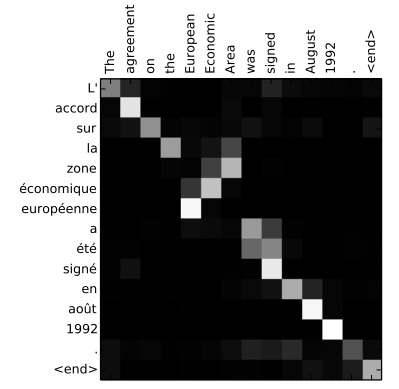
\includegraphics[height=0.5\linewidth]{alignments.png}
\caption{A sample alignment found by RNNsearch-50.}
    \label{A sample alignment found by RNNsearch-50}
\end{figure}
 \eenum

\subsubsection{Transformer Model}
\benum
\item 
 {Transformer Model}

\begin{center}``Attention is All You Need''\end{center}
$$***$$
The transformer model utilizes an encoder/decoder architecture with attention, but no recurrent connections!
 
Recall that training RNNs is not parallelizable and requires more memory for each example due to the recurrence.
 
Also achieves state-of-the-art performance on translation tasks.
 



\item 
 {NMT Model Comparison (December 2017)}.  Figure \ref{NMT Model Comparison}

\begin{figure}
\centering
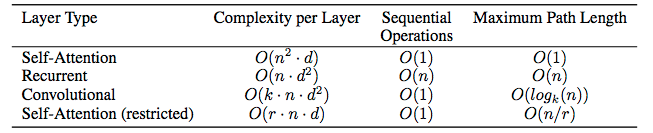
\includegraphics[height=0.15\linewidth]{nmt-compare3.png}
\caption{$n$ is sequence length, $d$ is representation dimension, $k$ is kernel size of convolutions, $r$ is the size of the neighborhood in restricted self-attention.}
    \label{NMT Model Comparison}
\end{figure}
Self-attention allows the Transformer to be trained in a more parallel fashion on GPU hardware. Typically, $d> n$.
 



\item 
 {Transformer Model}.  Figure \ref{Transformer Model}

\begin{figure}
\centering
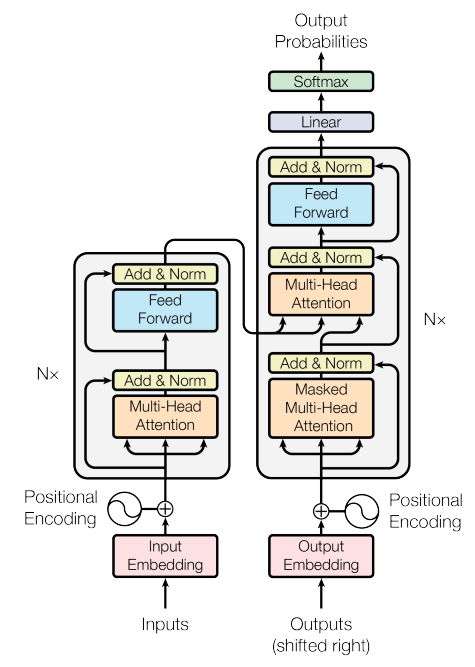
\includegraphics[width=0.45\linewidth]{transformer2.png}
    \caption{Transformer Model.}
    \label{Transformer Model}
\end{figure} 
% https://ai.googleblog.com/2017/08/transformer-novel-neural-network.html


No recurrent connections: the entire input sequence/output sequence so far is sent into the model at once (\href{https://ai.googleblog.com/2017/08/transformer-novel-neural-network.html}{demo}).
 
\begin{enumerate}
\item Input words get transformed into ``positional embeddings.''
\item For each encoder layer:
\begin{enumerate}
\item Apply multi-headed self-attention.
\item Send outputs through feedforward network.
\end{enumerate}
\item For each output word:
\begin{enumerate}
\item Transform all previous output words into positional embeddings.
\begin{enumerate}
\item Apply masked multi-headed self-attention.
\item Apply attention using the encoder outputs.
\item Send output through feedforward network.
\end{enumerate}
\item Transform output vector into the next word using linear and softmax layers.
\end{enumerate}
\end{enumerate}
 

\item 
 {Self-Attention}.  Figure \ref{Self-Attention}

Intuition: When the model processes a word, self-attention allows it to look at other positions in the input sequence to help it determine the optimal encoding for the word.
 
Example: ``The animal didn't cross the street because \textcolor{red}{it} was too tired.''
\begin{itemize}
\item
\href{https://colab.research.google.com/github/tensorflow/tensor2tensor/blob/master/tensor2tensor/notebooks/hello_t2t.ipynb}{Visualization}
\end{itemize}
\begin{figure}
\centering
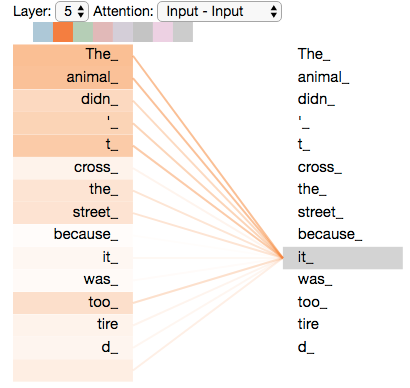
\includegraphics[height=0.4\linewidth]{self-attention.png}
    \caption{Self-Attention.}
    \label{Self-Attention}
\end{figure}
 

\item 
 {Self-Attention}.  Figure \ref{Self-Attention 1}

%An \textbf{attention function} maps a query and a set of key-value pairs to an output. The output is a weighted sum of the values, where the weights are computed by a compability function of the query with the corresponding key.
Step 1: Generate query, key, and value vectors for each embedding using learned matrices $W^Q$, $W^K$, $W^V$.
\begin{figure}
\centering
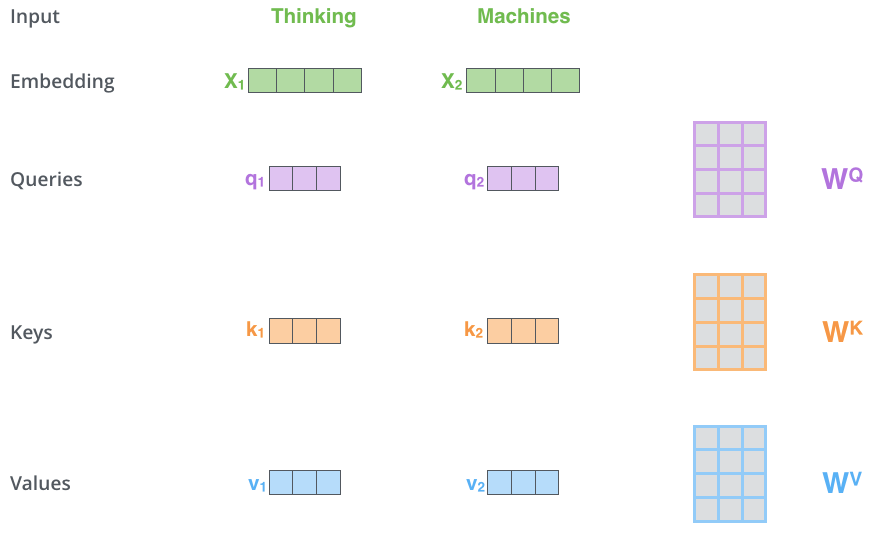
\includegraphics[height=0.5\linewidth]{self-attention1.png}
    \caption{Self-Attention 1.}
    \label{Self-Attention 1}
\end{figure}
 


\item  Figure \ref{Self-Attention 2}

%\textbf{Multi-headed attention} means learning $M$ attention layers in parallel, and combining the results using another learned matrix $W^Z$.
Step 2: Compute a score for each key-value pair. Normalize these weights to sum to 1, and compute the output as the weighted sum of the values.
\begin{figure}
\centering
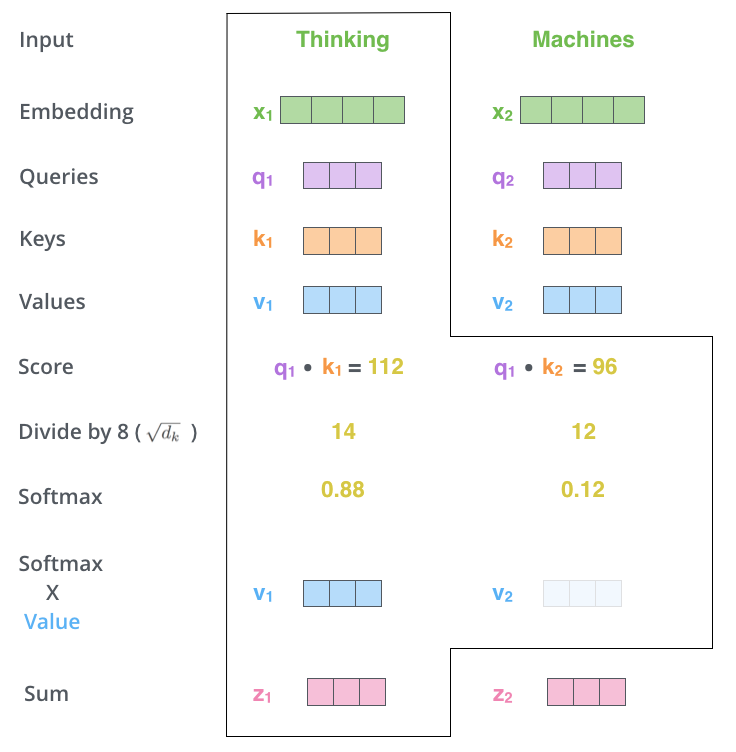
\includegraphics[height=0.55\linewidth]{self-attention2.png}
    \caption{Self-Attention 2}
    \label{Self-Attention 2}
\end{figure}
 

\item  Figure \ref{Self-Attention 3}

\textbf{Multi-headed attention} means learning $M$ attention layers in parallel (with different weight matrices).

Step 3 is combining the results using another learned matrix $W^O$.
\begin{figure}
\centering
\includegraphics[width=1\linewidth]{self-attention3.png}
    \caption{Self-Attention 3}
    \label{Self-Attention 3}
\end{figure} 
 

\item 
 {NMT Model Comparison (December 2017)}.  Figure \ref{TheT}

\begin{figure}
\centering
\includegraphics[height=0.3\linewidth]{nmt-compare2.png}
\caption{The Transformer outperforms other state-of-the-art models at a fraction of the training cost. FLOPS is floating point operations.}
\label{TheT}
\end{figure}
 

\item 
 {Future Directions for NMT}

Explore attention and CNNs as an alternative to RNNs.
 
Many active research areas in NMT, including:
\begin{enumerate}
\item Sub-word or character-level models.
\item Rare word problem.
\item Low-resource languages.
\item Efficient decoding.
\end{enumerate}

\item {References}

Pascanu, Mikolov, Bengio (2013) {On the difficulty of training recurrent neural networks}
 {\emph{arXiv preprint} arXiv:1211.5063}
 
Cho, Bahdanau, Bougares, Schwenk, Bengio (2014)
  {
  Learning Phrase Representations using RNN Encoder-Decoder for Statistical Machine Translation}
  {\emph{arXiv preprint} arXiv:1406.1078}
 
Bahdanau, Cho, Bengio (2015)
  {Neural Machine Translation by Jointly Learning to Align and Translate}
 {\emph{arXiv preprint} arXiv:1409.0473}
 
 Vaswani, Shazeer, Parmar, Uszkoreit, Jones, Gomez, Kaiser, Polosukhin (2017)
 {Attention Is All You Need}
 {\emph{arXiv preprint} arXiv:1706.03762}

\eenum

\subsection{Image + Text}


\benum
\item Models that combine images and text have a special feel of "intelligence". We are used to models for classifying images and translating text, but generating captions for an image, or answering questions aboout it, may be more unusual. This is in addition to the obvious practical importance of these tasks. 

\item 
Karpathy, Fei-Fei Li, Deep Visual-Semantic Alignments for Generating Image Descriptions
\benum 
\item Task: generate natural language descriptions of different image regions. Input image, output Regions+Captions. Figure \ref{Caption}

\begin{figure}
  \centering
  \includegraphics[scale=0.5]{Caption.png}
    \caption{Deep Visual-Semantic Alignments for Generating Image Descriptions}
    \label{Caption}
\end{figure}

\item Data:  image + sentence. These are weak labels (not segmented)

\item Alignment: input image and a sentence, output: score for how well they match

Segment: R-CNN. Map each region to 500-dimensional space.

Text: bidirectional RNN. Map each word of sentence to 500-dimensional space. 

Can compute similarity/inner product/alignment.

"since we are
ultimately interested in generating snippets of text instead
of single words, we would like to align extended, contigu-
ous sequences of words to a single bounding box.
To address this issue, we treat the true alignments as latent
variables in a Markov Random Field (MRF) where the binary interactions between neighboring words encourage an alignment to the same region"

\item "Multimodal Recurrent Neural Network for
generating descriptions". Generation: Input: image. Output: Embedding. 

Feed to RNN as a state variable. Output: Caption.

[Amazing that you can represent text and images in the same space.]
\eenum 

\item Visual Question Answering (Q+A)

\benum 
\item 
\eenum 

 
\eenum 

\section{Unsupervised learning}

\subsection{Setup}

\benum
\item Unsupervised learning: we have features $x_i$, but no outcomes $y_i$. We are trying to understand structure, summarize, compress, denoise, visualize, the data.

This data can be easier to collect. However, it can be more removed from the "end-goal" or "decision-making". In supervised learning we can make a yes/no decision that we can directly act on. In unsupervised learning, we are often making an intermediate decision. 

Most direct economic value comes from supervised learning, where we predict outcomes.


\item Classical statistics and statistical learning: 

Non-parametric density estimation: kernel methods, local polynomial methods

Dimension reduction: PCA, ICA, random projections

Clustering: k-means, EM


\item Connections with supervised learning: There is a rich set of connections to supervised learning. 

Reductions: Often unsupervised methods can be viewed as reductions to supervised learning. e.g., in dimension reduction, we try to find a function $f$ of the data (in some class), so that there is some other function $g$ of the data (in some class), so that $g(f(X))$ approximates $X$ well. 

Semi-supervised Learning: Given a (small) amount of labeled data and a (large) amount of unlabeled data, learn predictor. Example: learning parse trees, image search, ...

Self-supervised learning: Construct your own supervision. For instance, predict some part of the image. Predict the next frame in a video. Yann LeCun advocates that this is important, because "the future will not be supervised".

\eenum 

\subsection{PCA, AE, VAE}


\benum
\item PCA. Widely used for exploratory data analysis


Data matrix $X$, $n \times p$, has $p$ features of $n$ samples (e.g., genomic features of samples from Europe). Center each column of $X$.

Principal Component Analysis (PCA): Find linear combinations 
$$f = Xv = \sum_i v_i X_i$$ 
of features that maximize variance. 


Sequentially, subject to orthogonality constraints. First PC: maximize empirical variance 
\begin{align*}
\max_v\,\,  &\Var{Xv} = n^{-1} v^\top X^\top Xv\\
s.t.\,\,&v^\top v=1
\end{align*}
Nonconvex optimization problem. Solution $v$: top eigenvector of sample covariance matrix $\hSigma = n^{-1} X^\top X$.

Variance: largest eigenvalue of $\hSigma$. 
Similarly at all steps: PC scores - eigenvectors, variances - eigenvalues. 

Equivalently, can write all steps in one as 
\begin{align*}
\max_V&\,\, \tr (V^\top X^\top XV)\\
s.t.\,\,&V^\top V=I_k
\end{align*}
or 
\begin{align*}
\min_V&\,\,\|X(I-VV^\top)\|_{Fr}^2\\
s.t.\,\,&V^\top V=I_k
\end{align*}

This last reformulation can be viewed as a reduction to supervised learning. We try to find a function $Z:=f(X)=XV$ of the data that reduces the dimension from $p$ to $k$, so that the pseudoinverse $g(Z) = ZV^\top$ approximates $X$ well. In this case, we impose the constraint that $VV^\top$ is an orthogonal projection matrix. However, if we are looking for a linear subspace (manifold), that best approximates the data, we automatically get that the approximation operation has to be a linear projection. So, effectively, PCA = "Best Linear Subspace."


\item Autoencoders (AE): Relax the linear maps to more general maps, e.g., neural networks.  Figure \ref{ae0},

\begin{align*}
\min&\,\,\sum_i \|x_i-g(z_i,W_g)\|^2\\
s.t.\,\,&z_i = f(x_i,W_f)
\end{align*}

\begin{figure}
  \centering
  \includegraphics[scale=0.5]{ae0.png}
    \caption{AE}
    \label{ae0}
\end{figure}

Note: Encoder and Decoder

Training: backprop

Empirical results?

Probably not good at generating new meaningful images.

\item Variational Autoencoders  (VAE). Figure \ref{vae},

\begin{figure}
  \centering
  \includegraphics[scale=0.6]{vae.png}
    \caption{VAE}
    \label{vae}
\end{figure}

Instead, model the distribution of the latent variable $z$ probabilistically, and try to fit models for the probability distributions $p(x|z), q(z|x)$.

Parametrize:
\benum 
\item  Prior distribution $p_\theta(z)$.
\item  Conditional distribution $p_\theta(x|z)$.
\eenum 

High-level goal: maximize (marginal) likelihood. 

$$\max_\theta \sum_i \log p_\theta(x_i) 
$$
Express in terms of latent variable $z$

$$p_\theta(x) 
= \int 
p_\theta(z)p_\theta(x|z)dz
$$
In principle, if we maximize over $\theta$, then theoretically we obtain the posterior distribution as $p(z|x) = p(x|z)p(z)/p(x)$. How can we train this model?

The direct approach has issues. We need to approximate the $z$-integral by a quadrature, which can become prohibitive in high dimensions.

\item Different approach:
The parameters of the VAE can be estimated efficiently in the stochastic gradient variational Bayes (SGVB) framework, where the variational lower bound of the log-likelihood is used as a surrogate objective function. 

First we introduce and parametrize an approximation to the posterior $p(z|x)$:
\benum 
\item  Conditional distribution $q_\phi(z|x)$.
\eenum 

See Figure \ref{svae} for the sampling process of VAEs:
\begin{figure}[H]\centering
\includegraphics[width=12cm]{VAE_P1}
\caption{Sampling process of VAEs.}
   \label{svae}
\end{figure}




The variational lower bound is written as:

\begin{align*}
	\log p_{\theta}(x) %&= \mathbb{KL}[q_{\phi}({z}|{x})||p_{\theta}({z}|{x})] + \mathbb{E}_{q_{\phi}({z}|{x})}[-\log q_{\phi}({z}|{x})+ \log p_{\theta}({x}, {z})]\\
	&\geq\mathbb{E}_{z}[\log p_{\theta}(x|z)] - \mathbb{KL}[q_{\phi}(z|x)||p_{\theta}(z)]
\end{align*}




%------------------------------------------------

\item 

Here are the details. We want to maximize the data likelihood:
\begin{equation*}
	p_{\theta}(x) = \int p_{\theta}(z)p_{\theta}(x|z)dz
\end{equation*}
\begin{align*}
	\log p_{\theta}(x) &= \mathbb{E}_{z\sim q_{\phi}(z|x)}[\log p_{\theta}(x)]\\
	&=\mathbb{E}_{z}[\log\frac{p_{\theta}(x|z)p_{\theta}(z)}{p_{\theta}(z|x)}]\\
	&=\mathbb{E}_{z}[\log\frac{p_{\theta}(x|z)p_{\theta}(z)}{p_{\theta}(z|x)}\frac{q_{\phi}(z|x)}{q_{\phi}(z|x)}]\\
	&=\mathbb{E}_{z}[\log p_{\theta}(x|z)] - \mathbb{E}_{z}[\log\frac{q_{\phi}(z|x)}{p_{\theta}(z)}] + \mathbb{E}_{z}[\log\frac{q_{\phi}(z|x)}{p_{\theta}(z|x)}]\\
	&=\mathbb{E}_{z}[\log p_{\theta}(x|z)] - \mathbb{KL}[q_{\phi}(z|x)||p_{\theta}(z)] + \mathbb{KL}[q_{\phi}(z|x)||p_{\theta}(z|x)]
\end{align*}
The last KL-Divergence is greater than or equal to 0. Define:
\begin{equation*}
	\mathcal{L}(x, \theta, \phi) = \mathbb{E}_{z}[\log p_{\theta}(x|z)] - \mathbb{KL}[q_{\phi}(z|x)||p_{\theta}(z)]
\end{equation*}

Then $\log p_{\theta}(x) \geq \mathcal{L}(x, \theta, \phi)$. 
In VAEs we try to maximise the lower bound

\begin{align*}
\sum_{i=1}^n \mathcal{L}(x_i, \theta, \phi)
\end{align*}

We can try to approximate the expectations by sampling. Both expectations are over $z$, so we can sample several independent $z_j$ (using the current paramters $\phi_t$) and use plug-in estimators for the expectations. 


$\mathbb{E}_{z}[\log p_{\theta_t}(x|z)]
\approx
m^{-1}\sum_{j=1}^m \log p_{\theta_t}(x|z_j)
$

$
\mathbb{KL}[q_{\phi_t}(z|x)||p_{\theta_t}(z)]\approx
m^{-1}\sum_{j=1}^m
\log\frac{q_{\phi_t}(z_j|x)}{p_{\theta_t}(z_j)}
$

We do this for all $x=x_i$, and take gradient steps with respect to $\phi,\theta$. The problem with this is that it does not give the correct gradient with respect to $\phi$, as the expectation depends on $\phi$ and we have sampled according to that, so the derivative of the sampling will not give the dependence of the probability measure on $\phi$

%------------------------------------------------








%------------------------------------------------

\item 
Reparameterization trick. The key to the problem is the reparametrization trick, which evaluates $z$ as a deterministic function of $\phi$ as $z = g(\phi,x,\ep)$ instead of sampling from a probability distribution parametrized by $\phi$. Then we can easily evaluate the derivative wrt $\phi$ by backprop. See Figure \ref{Reparam}


\begin{figure}[H]\centering
\includegraphics[width=10cm]{Reparam}
\caption{Reparameterization trick for VAEs.}
\label{Reparam}
\end{figure}

Putting it all together: See Figure \ref{VAE_Process}

%----------------------------------------------
\begin{figure}[H]\centering
\includegraphics[width=12cm]{VAE_Process}
\caption{Framework of VAEs.}
\label{VAE_Process}
\end{figure}





%------------------------------------------------

\item 

Application on Faces:
\begin{figure}[H]\centering
\includegraphics[width=1cm]{face2.eps}
\includegraphics[width=1cm]{face150.eps}
\includegraphics[width=1cm]{face268.eps}
\includegraphics[width=1cm]{face700.eps}
\includegraphics[width=1cm]{face990.eps}
\includegraphics[width=1cm]{face1004.eps}
\includegraphics[width=1cm]{face1354.eps}
%\caption{Original faces we use to train the model}
\end{figure}

\begin{figure}[H]\centering
\includegraphics[width=6cm]{face56.eps}
\caption{Generated faces}
\end{figure}

% \begin{figure}[H]\centering
% \includegraphics[width=4cm]{face910.eps}
% \caption{Generated faces}
% \end{figure}


\url{https://distill.pub/2017/aia/}




\eenum 

 
\subsection{Generative adversarial networks (GAN)}

\benum
\item \emph{Generative adversarial networks (GANs)} are a method proposed first for unsupervised learning (Goodfellow et al, 2014). Considered by some experts to be the most important development in machine learning in the last 20 years. 
\begin{figure}
  \centering
  \includegraphics[scale=0.4]{gan.png}
    \caption{GAN}
    \label{gan}
\end{figure}
%\eenum

\item Example results: Figures \ref{gan1}, \ref{gan2}

\begin{figure}
  \centering
  \includegraphics[scale=0.25]{gan1.jpg}
    \caption{GAN Example}
    \label{gan1}
\end{figure}
%\eenum
\begin{figure}
  \centering
  \includegraphics[scale=0.3]{gan2.jpg}
    \caption{GAN Example}
    \label{gan2}
\end{figure}

\item 
 Want to learn density of images. In classical statistics, one would approach this problem by fitting a density $P_\theta$ from a given family (parametric or non-parametric) to the empirical data distribution. 

 GANs learn a density by learning a \emph{generator} $G$ and a \emph{discriminator} $D$. The generator is an algorithm to sample from the density of images, while the discriminator is an algorithm to distinguish the real from the generated images. By simultaneously training the two \emph{adversaries}, we end up with both a good classifier and a good generator. (Figure \ref{gan})
 

 \item 
More formally, let 

\bitem
 \item 

$P_n$: data distribution
 \item 

$G$: a generator that takes in a random vector $Z$, and produces a generated sample $G(Z) \sim P_G$
 \item 

$D$: a discriminator that takes in a datapoint, and is supposed to return close to 1 for real data, and close to 0 for generated data (aka classifier)
\eitem 
The original GAN objective: 

$$\min_G\max_D V(D,G) = \E_{P_n} \log D(X) + \E_{G} \log[1-D(G(Z))] $$
 
The reason why these are called networks is that $G,D$ are both taken to be neural networks

\item Training initializes both networks randomly, and then performs \emph{alternating gradient updates} as follows.  Iterate:
\benum
\item Generate a few samples $G(Z_i)$ from the current density (say $m$ samples, and call the distribution $G_k$)
\item Update the discriminator parameters  using a gradient step on the generated and real data (this update depends on the current generator)

Specifically, the objective is

\begin{align*}
\hat V(G) & = \E_{P_n} \log D(X) + \E_{G_k} \log[1-D(G(Z))]\\
&= n^{-1}\sum_{i=1}^n\log D(X_i) + m^{-1}\sum_{j=1}^m \log[1-D(G(Z_j))]
\end{align*}

We compute the gradient of this wrt the parameters $\theta$ of the net $D$ via backprop. 


\item Update the generator using a gradient step to better match the true density (the gradient step now depends on the current discriminator)
\eenum

\item Some basic results: 

Proposition (Goodfellow et al, 2014). For a fixed generator $G$, the \emph{optimal discriminator} $D$ has the form 

$$D^*(x) = \frac{p_n(x)}{p_n(x)+p_G(x)},$$

where $p_n$ is the data density, and $p_G$ is the generated density. The optimal discriminator can be defined arbitrarily outside of the support of the two densities. 

Consider next the \emph{equilibrium value} of the game, i.e., the solution to the minimax problem: 

$$\min_G C(G)  = V(D^*,G) $$
 
One can check $G(G) = 2 JS(P_n \| P_G) - \log(4)$, where $JS$ is the \emph{Jensen-Shannon divergence}, 

$$JS(P\| Q) = \frac12 KL(P\|(P+Q)/2)+ \frac12 KL(Q\|(P+Q)/2).$$ 

Recall that the \emph{Kullback-Leibler (KL) divergence} is 

$$KL(P\|Q) = \E_P \log(P(X)/Q(X)).$$


Therefore, the original GAN can be viewed as minimizing 

$$\min_G JS(P_n \| P_G) $$
 
By the well-known properties of JS divergence, within the class of distributions that have a density wrt $P_G$, this is minimized at $P_G$. 


\item Now we can see that this is just a form of risk minimization. Later work considered other versions, motivated by the numerical instability of the original GANs. For instance \emph{Wasserstein GAN (WGAN)} (Arjovsky et al, 2017) solves

$$ \min_{G} d(P_G ,P_n) =  \min_{G} \max_{F\in \mathcal{F}}[ \E_{P_G} F - \E_{P_n} F]$$

Here $d(P,Q)$ is the \emph{Wasserstein-1 metric}, or \emph{earth-mover distance}, and $ \mathcal{F}$ is the class of 1-Lipshitz functions defined on the domain $S$ where all probability distributions reside: 

$$\mathcal{F} = \{F: S \to \R: |F(X)- F(Y)| \le \|X-Y\|\}$$

To solve, we follow the same alternating gradient scheme as before. Iteratively, 
\benum
\item Update $F$
\item Update $P$
\eenum
Approximate $\E$ by sampling.

[Justify]

\item \emph{Stability?} Training GANs is notoriously unstable. How can they be made stable?

Hacks: \url{https://github.com/soumith/ganhacks}


\item \emph{Mode collapse.} GANs often suffer from a form of underfittign known as mode collapse. Specifically, they drop modes of a distribution, and generate only from the rest. Figure \ref{mc}. %[Arora et al]

\begin{figure}
  \centering
  \includegraphics[scale=0.3]{mc.png}
    \caption{Mode collapse. Top: "Unrolled GAN", bottom: standard GAN}
    \label{mc}
\end{figure}

\item GauGAN
\eenum

\subsection{Wasserstein GAN}

\benum
\item {Notation}.
 Let $\mathcal{X}$ be a compact metric space. Let $\Sigma$ denote all Borel sets of  $\mathcal{X}$. Let $Prob(\mathcal{X})$ denote the space of probability measures defined on $\mathcal{X}$. Now we define some elementary distances and divergences between two distributions $P_r, P_g \in Prob(\mathcal{X})$


\item {The \emph{Total Variation} (TV) distance} is
$$ \delta(P_r, P_g)= \sup_{A\in \Sigma} {|P_r {(A)}-P_g {(A)}|}$$





\item {The \emph{Kullback-Leibler} (KL) divergence} is
 $$ KL(P_r \|P_g)= \int_\mathcal{X} \log(\frac{dP_r}{dP_g})dP_r$$
 Note that $P_r$ needs to be absolutely continuous with respect to $P_g$. Actually the KL divergence is not a distance since it is asymmetric.
 




\item {The \emph{Jensen-Shannon} (JS) divergence} is
$$ JS(P_r,P_g)=KL(P_r \|P_m)+ KL(P_g \|P_m)$$
where $P_m$ is $\frac{P_r+P_g}{2}$. This divergence is symmetric and always well-defined.






\item {The \emph{Earth-Mover} (EM) distance or Wasserstein-1 distance} is
$$W(P_r,P_g)=\inf_{\gamma \in \prod(P_r,P_g)} E_{(x,y)\sim \gamma} [\|x-y\|]$$
where $\prod(P_r,P_g)$ denote the set of all joint distributions $\gamma(x,y)$ whose marginals are respectively $P_r$ and $P_g$. Intuitively, $\gamma(x,y)$ indicates how much "mass" must be transported form x to y in order to transform the distribution $P_r$ into the distribution $P_g$. The EM distance the is the "cost" of the optimal transport plan.





\item { \emph{Example} (learning parallel lines)}.
Let $Z\sim U[0,1]$ the uniform distribution on the unit interval. $P_0$ denotes the distribution of $(0,Z)\in R^2$ and $P_\theta$ denotes the distribution of $(\theta,Z)\in R^2$. Then:
\begin{itemize}
     \item $\delta(P_0,P_\theta)=\left\{ \begin{array}{ll}
             1 & if \,\, \theta \not= 0,\\
             0 & if \,\, \theta =0 \end{array}\right.$
     
   \end{itemize}






\item {}
\begin{itemize}
     \item $KL(P_0,P_\theta)=KL(P_\theta, P_0)=\left\{ \begin{array}{ll}
             \infty & \textnormal{ if } \theta \not= 0,\\
             0 & \textnormal{ if } \theta =0 \end{array}\right.$
    \item $ JS(P_0,P_\theta)=\left\{ \begin{array}{ll}
             \log(2) & \textnormal{ if } \theta \not= 0,\\
             0 & \textnormal{ if } \theta =0 \end{array}\right.$
   \item $ W(P_0,P_\theta)= |\theta|$
\end{itemize}





\item {\emph{Theorem 1.}}
 Let $P_r$ be a fixed distribution over $\mathcal{X}$. Let $Z$ be a random variable (e.g. Gaussian) over another space $\mathcal{Z}$. Let $g: \mathcal{Z}\times R^d \rightarrow \mathcal{X}$ be a function, denoted $g_\theta (z)$. Let $P_\theta$ denote the distribution of $g_\theta (Z)$. Then:\\
 1. If $g$ is continuous in $\theta$, so is $W(P_r,P_\theta)$.\\
 2. If $g$ is locally Lipschitz and satisfies some regularity assumption, then $W(P_r,P_\theta)$ is continuous everywhere, and differentiable almost everywhere.\\
 3. Statements 1-2 are false for the JS divergence $JS(P_r,P_\theta)$




\item {Remarks}.

\benum 
\item   $g_\theta(z)$ is locally Lipschitz iff for a given pair $(\theta, z)$ there is a constant $L(\theta, z)$ and an open set $U$ s.t. for every $(\theta', z')\in U$ we have $$\|g_{\theta} (z)-g_{\theta'}(z')\| \le L(\theta, z)(\|\theta-\theta'\|+\|z-z'\|) $$
\item   suppose $g_\theta(z)$ is locally Lipschitz, then we say that $g_\theta(z)$ satisfies the \emph{regularity assumption} for a certain probability distribution p over $\mathcal{Z}$ if the local Lipschitz constants $L(\theta, z)$ satisfy $E_{z\sim p} [L(\theta, z)]< +\infty$
\eenum





\item {\emph{Corollary 1.}}
 Let $g_\theta$ be any feedforward neural network parametrized by $\theta$, and $p(z)$ a prior over z such that $E_{z\sim p(z)}[\|z\|]<\infty$(e.g. Gaussian, uniform, etc) then $g_\theta(z)$is locally Lipschitz and satisfies regularity assumption, therefore $W(P_r,P_\theta)$ is continuous everywhere, and differentiable almost everywhere.
 





\item {\emph{Theorem 2.}}
 let P be a distribution on a compact space $\mathcal{X}$ and $(P_n)_{n\in N}$ be a sequence of distributions on $\mathcal{X}$. Then, considering all limits as $n \rightarrow \infty$, \\
 1. The following statements are equivalent 
 \begin{itemize}
  \item $\delta(P_n, P)\rightarrow 0$ with $\delta$ the total variation distance.
  \item $JS(P_n, P)\rightarrow 0$ with JS the \emph{Jensen-Shannon} divergence.
  \end{itemize}

 2. The following statements are equivalent
 \begin{itemize}
  \item $W(P_n, P)\rightarrow 0$.
  \item $P_n \rightarrow^{\mathcal{D}} P$ where $\rightarrow^{\mathcal{D}}$ represents convergence in distribution (weak convergence).
  \end{itemize}


3. $KL(P_n\|P)\rightarrow 0$ or $KL(P\|P_n)\rightarrow 0$ imply the statement in 1.\\
4. The statements in 1 imply the statements in 2.


\eenum

\subsubsection{WGAN}
\benum



\item 
Theorem 2 indicates that EM distance or Wasserstein-1 distance has better properties when optimized than JS divergence. However the infimum in the definition of EM distance is highly intractable. However the Kantorovich-Rubinstein duality theorm (Villani. Optimal transport: Old and New) tells us 
$$W(P_r,P_\theta)= \sup_{\|f\|_L\le 1} {\{\E_{x\sim P_r}[f(x)]-\E_{x\sim P_\theta}[f(x)]\}}$$
where the supremum is over all the 1-Lipschitz functions $f: \mathcal{X}\rightarrow R$ 


\item 
Now if we have a parameterized family of functions $\{f_w\}_{w\in \mathcal{W}}$ that are all K-lipschitz for some K, we could consider the problem 
$$\sup_{w\in \mathcal{W}} {\{\E_{x\sim P_r}[f_w(x)]-\E_{z\sim p(z)}[f_w(g_\theta(z))]\}}$$






\item {\emph{Theorem 3.}}
Let $P_r$ be any distribution. Let $P_\theta$ be the distribution of $g_\theta(Z)$ with Z a random variable with density p and $g_\theta$ a function satisfying the \emph{regularity assumption}. Then there is a solution $f: \mathcal{X}\rightarrow R$ to the problem 
$$\max_{\|f\|_L \le 1} {\{\E_{x\sim P_r}[f(x)]-\E_{x\sim P_\theta}[f(x)]\}}$$
and we have
$$\nabla_\theta W(P_r,P_\theta)=-\E_{z\sim p(z)}[\nabla_\theta f(g_\theta(z))]$$
when both terms are well defined. (They are well-defined under the condition of this theorem.)




\item {\emph{How can we find the optimal f?}}
One way to solve this problem is that train a neural network parameterized with weights w lying in a compact space $\mathcal{W}$ (it can make sure all the functions $f_w$ are K-Lipschitz for some K that only depends on  $\mathcal{W}$ and the critic architecture) and then backprop through $-\E_{z\sim p(z)}[\nabla_\theta f(g_\theta(z))]$, as we would do with a typical GAN.\\
~\\
To have parameters w lie in a compact space, we could clip the weights to a fixed box (say $\mathcal{W}=[-0.01,0.01]^l$) after each gradient update. Figures \ref{wgan}, \ref{gan_alg}




 
\begin{figure}[h!]
  \caption{WGAN algorithm}
  \centering
  \includegraphics[width=0.8\textwidth]{WGAN_algorithm.png}
  \label{wgan}
\end{figure}




\begin{figure}[h!]
  \caption{GAN algorithm}
  \centering
  \includegraphics[width=0.8\textwidth]{GAN_algorithm.png}
    \label{gan_alg}
\end{figure}



\item {\emph{Some analysis for the WGAN algorithm}}.
There are only four modifications that WGAN made on the basic GAN framework:
~\\
1. Removing the sigmoid activation function in the last layer.\\
2. Removing the log in the loss function of G/D models.\\
3. Clipping the parameters so that their absolute values are smaller than a constant c.\\
4. Not using any optimization methods based on momentum (like Adam method); RMSProp is the recommended method.





\item {\emph{Benefits of WGAN}}
1. Wasserstein distance is highly correlated with the generator's convergence and sample quality. Figure \ref{wass_qual}
\begin{figure}[h!]
  \centering
  \includegraphics[width=0.6\textwidth]{WassGAN_loss_function.jpg}
      \caption{Wasserstein distance is highly correlated with the generator's convergence and sample quality.}
    \label{wass_qual}
\end{figure}




\item {\emph{Benefits of WGAN}}
2. Improved stability
\begin{itemize}
  \item It has no sign of mode collapse in experiments.
  \item The generator can still learn when the critic perform well.
  \item WGANs are more robust than GANs when one varies the architectural choice for the generator.
  \end{itemize}
\eenum



\subsubsection{Gradient penalty}

\benum
\item {\emph{Difficulties of WGAN}}.
 Weight clipping is a clearly problematic way to enforce a Lipschitz constraint. It has two difficulties:
 ~\\
\item  Without careful tuning of the clipping threshold c, it may result in either vanishing or exploding gradients. Figure \ref{explode}







 \begin{figure}[h!]
  \centering
  \includegraphics[width=0.5\textwidth]{explode.png}
  \caption{(left) gradient norms of deep WGAN critics during training on the Swiss Roll dateset either expolde or vanish when using weight clipping, but not when using a gradient penalty. (right) Weight clipping pushes weights towards the extremes of the clipping range, unlike gradient penalty.}
  \label{explode}
  \end{figure}




\item Weight clipping reduces the capacity of the critic f and limits the capability to model complex functions. Figure \ref{value} 
\begin{figure}[h!]
  \centering
  \includegraphics[width=0.8\textwidth]{value.jpg}
    \caption{Weight clipping reduces the capacity of the critic f and limits the capability to model complex functions.}
  \label{value}
 \end{figure}




\item {\emph{Proposition 1.}}
Let $P_r$ and $P_g$ be two distributions on $\mathcal{X}$, a compact metric space. Then there is a 1-Lipschitz function $f^*$ which is the optimal solution of 

$$\max_{\|f\|\le 1} {\{\E_{y\sim P_r}[f(y)]-\E_{x\sim P_g}[f(x)]\}}.$$ 

Let $\pi$ be the optimal coupling between $P_r$ and $P_g$, defined as the minimizer of $W(P_r,P_g)=\inf_{\pi\in \prod(P_r,P_g)}\E_{(x,y)\sim\pi}[\|x-y\|]$ where $\prod(P_r,P_g)$ is the set of joint distributions $\pi(x,y)$ whose marginals are $P_r$ and $P_g$, respectively. Then if $f^*$ is differentiable, $\pi(x=y)=0$, and $x_t=tx+(1-t)y$ with $0\le t\le 1$, it holds that 

$$P_{(x,y)\sim\pi}[\nabla f^*(x_t)=\frac{y-x_t}{\|y-x_t\|}]=1.$$ 




\item {\emph{Corollary 1.}}
$f^*$ has gradient norm 1 almost everywhere under $P_r$ and $P_g$.




\item {\emph{WGAN-GP}}.
 A differentiable function is 1-Lipschtiz if and only if it has gradients with norm at most 1 everywhere, so we consider directly constraining the gradient norm of the critic’s output with respect to its input. To circumvent tractability issues, we enforce a soft version of the constraint with a penalty on the gradient norm for random samples $\hat{x}\sim P_{\hat{x}}$.




\item {\emph{New objective}}
$$L=E_{\Tilde{x}\sim P_g}[D(\Tilde{x})]-\E_{x\sim P_r}[D(x)]+\lambda E_{\hat{x}\sim P(\hat{x})}[(\|\nabla_{\hat{x}}D(\hat{x})\|_2 -1)^2]$$





\item {\emph{Algorithm}}. Figure \ref{wgan_gp}
\begin{figure}[h!]
  \centering
  \includegraphics[width=0.85\textwidth]{WGAN_GP.png}
    \caption{WGAN Gradient Penalty.}
  \label{wgan_gp}
 \end{figure}




\item {\emph{Some analysis}}.
1. We implicitly define $P_{\hat{x}}$ sampling uniformly along straight lines between
pairs of points sampled from the data distribution $P_r$ and the generator distribution $P_g$. Given that enforcing the unit gradient norm constraint everywhere is intractable, enforcing it only along these straight lines seems sufficient and experimentally results in good performance.

2. Penalty coefficient: All experiments in the paper use $\lambda=10$, which we found to work well across a variety of architectures and datasets ranging from toy tasks to large ImageNet CNNs.\\
3. No critic batch normalization. Because we penalize the norm of the critic’s gradient with respect to each input independently, and not the entire batch. 





\item {\emph{Experimental results}}.
WGAN-GP enhances training stability. As shown below, when the model design is less optimal, WGAN-GP can still create good results while the original GAN cost function fails. Figure \ref{wgan_gp_exp}

\begin{figure}[h!]
  \centering
  \includegraphics[width=0.7\textwidth]{experiment.png}
    \caption{WGAN Gradient Penalty. Experimental results}
  \label{wgan_gp_exp}
 \end{figure}

\item {\emph{References}}.

1. M. Arjovsky and L. Bottou. Towards principled methods for training generative adversarial networks. 2017.\\
2. M. Arjovsky, S. Chintala, and L. Bottou. Wasserstein gan. arXiv preprint arXiv:1701.07875. 2017.\\
3. Ishaan Gulrajani, Faruk Ahmed, Martin Arjovsky, Vincent Dumoulin, Aaron Courville1, Improved Training of Wasserstein GANs. 2017\\

\eenum






\section{Sequential decision-making: from bandits to deep reinforcement learning}

\subsection{Intro}

\benum

\item {Setup}
\bitem
\item Question: How to learn from experience that accumulates gradually over time?

\item Specifically: How to make decisions?

\eitem




\item {Bandits - a clean model}. Figure \ref{band_ex}.
\begin{figure}[h!]
\begin{center}
\includegraphics[width=0.4\paperwidth]{bandits}
    \caption{Bandit example}
    \label{band_ex}
\end{center}
\end{figure}



\item {Online advertising}. Figure \ref{online_ad}.
\begin{figure}[h!]
\begin{center}
\includegraphics[width=0.5\paperwidth]{online_ad}
    \caption{Online advertising}
    \label{online_ad}
\end{center}
\end{figure}



\item {Adaptive clinical trials}. Figure \ref{ada_ct}.
\begin{figure}[h!]
\begin{center}
\includegraphics[width=0.5\paperwidth]{ada}
    \caption{Adaptive clinical trials}
    \label{ada_ct}
\end{center}
\end{figure}



\item {Robotics}. Figure \ref{robo}.
\begin{figure}[h!]
\begin{center}
\includegraphics[width=0.3\paperwidth]{robo}
    \caption{Robotics}
    \label{robo}
\end{center}
\end{figure}




\item {Examples}
\bitem
\item Healthcare
\bitem
\item Adaptive clinical trials, e.g., oncology
\item mHealth, e.g., smoking, stress, exercise
\eitem
\item Web
\bitem
\item online ads, e.g., Microsoft, Google
\item dynamic pricing
\item A/B testing (different versions of website)
\item recommender systems: news, products
\eitem

\eitem



\item {Examples}
\bitem
\item Robotics
\bitem
\item Planning, search, control 
\eitem
\item Game playing
\bitem
\item Classical games: Chess, Go
\item Computer games
\eitem
\item ...
\eitem

\eenum

\subsection{Bandits}

\benum

\item {Setup}
\bitem
\item \emph{Time} $t=1,2,\ldots,T$
\item Need to choose an \emph{arm} $A_t \in  1, 2, \ldots, K$, 
\item Observe \emph{reward} $R_t$, which depends on the arm chosen
\item Goal: maximize \emph{returns}
\beqs
\max \sum_{t=1}^T R_t
\eeqs
\eitem



\item {Setup (2)}
\bitem
\item Simplest setting: rewards are random, and distribution only depends on the arm. $R_t|A_t = k \sim P_k$ (independently of the past). 
\item known as \emph{Stochastic bandits}
\item At each timestep, we have available the entire \emph{history} of previous actions and rewards $A_1,R_1,A_2,R_2,\ldots, A_{t-1}, R_{t-1}$
\item Our \emph{policy} (denoted $\pi$) chooses an action, in a possibly randomized way 
\eitem



\item {Rewards}. Figure \ref{rewards}.
\begin{figure}[h!]
\begin{center}
\includegraphics[width=0.3\paperwidth]{den}
    \caption{Reward distribution for two arms}
    \label{rewards}
\end{center}
\end{figure}




\item {How to act? Any ideas?}
\bitem
\item Recall: we have available the entire history of previous actions and rewards $A_1,R_1,A_2,R_2,$ $\ldots, A_{t-1}, R_{t-1}$
\item we need to choose arms in $1,\ldots,K$ to maximize sum of rewards. Rewards have a specific distribution for each arm.
\eitem



\item {Some possible policies}
\bitem
\item Initially explore all arms, then choose best (exploit) - (ETC)
\item Initially explore uniformly, then explore according to how promising the arms are - (Thompson sampling, Boltzmann/softmax, $\ep$-greedy)
\item Estimate an upper confidence bound on the mean reward for each arm, and be greedy - UCB
\eitem



\item {Notes}
\bitem
\item Balance \emph{exploration} and \emph{exploitation}
\item Separating them is suboptimal
\item In practice the other algorithms are quite similar (if tuned)
\eitem



\item {Measuring success--the notion of regret}
\bitem
\item In the stochastic case, assume $R_t \in [0,1]$ (or sub-Gaussian)
\item Focus only on the \emph{mean} rewards $\mu_k = \E_{P_k} R_t$
\item An oracle policy would choose the best arm at each step: 
\beqs
k^* = \arg\max_k \mu_k
\eeqs
and $\mu_{k^*} = \mu^*$
\item A more refined comparison between policies is given by the notion of \emph{regret}: the difference between the optimal action and the given policy:
\beqs
r_T = \max_k\E_{A_t=k} \sum_{t=1}^T R_{t} - \E_{\pi}\sum_{t=1}^T R_t
\eeqs
Or
\beqs
r_T = T \mu^* - \E_{\pi}\sum_{t=1}^T R_t
\eeqs
\eitem



\item {Regret}
\bitem 
\item Regret $r_T = T \mu^* - \E_{\pi}\sum_{t=1}^T R_t$
\item Minimizing regret is equivalent to maximizing return. But this is a more fine-grained measure, allows more careful comparison of policies
\item Minimize regret - important life lesson :)
\eitem

\eenum

\subsubsection{Policies and regret analysis}

\benum

\item {Explore then commit (ETC)}
\bitem 
\item ETC policy
\benum
\item {\it Explore}: Choose each arm $m$ times
\item {\it Exploit}: Choose best arm afterwards (for $T-Km$ times)
\eenum
\item {\bf Theorem}: Suppose $K=2$, and let $\Delta = |\mu_1-\mu_2|$. The regret of ETC is 
\beqs
r_T \le m\Delta + T\Delta \exp\left(-\frac{m\Delta^2}{4}\right)
\eeqs
\item Optimal $m = \lceil\frac{4}{\Delta^2}\log(\frac{T\Delta^2}{4})\rceil$ - after this many steps, probability of error is small
\item Achieves regret
\beqs
r_T \le \frac{4}{\Delta}\left[\log(\frac{T\Delta^2}{4})+1\right] + \Delta 
\eeqs
\item Worst case $\Delta \sim T^{-1/2}$, worst case regret
\beqs
r_T  = O(T^{1/2}) 
\eeqs
\eitem



\item {Notes on ETC}
\bitem 
\item We say that ETC attains regret $T^{1/2}$
%\item Proof idea
\item Proof: See tutorial by Lattimore and Szepesvari
\item Optimal up to order for $K=2$ (but not the right constant)
\item Issues
\bitem 
\item Non-adaptive: need to know $T,\Delta$ (hard for $K>2$)
\item Spend a lot of time not learning
\eitem

\eitem




\item {Optimism Principle}. Figure \ref{opti}.
\begin{figure}[h!]
\begin{center}
\includegraphics[width=0.25\paperwidth]{opti}
    \caption{Optimism Principle}
    \label{opti}
\end{center}
\end{figure}




\item {Optimism Principle - UCB Algorithm}
\bitem 
\item Upper Confidence Bound (UCB): Estimate an upper confidence bound on the mean reward for each arm, and be greedy
\item Let $T_k(t)$ be the number of times action $k$ was chosen until time $t$
\item Define the \emph{index} (or UCB) of arm $k$ at time $t$:
\beqs
\gamma_{k}(t)  = \hmu_k(t) + \sqrt{\frac{2\log(t^3)}{T_k(t)}}
\eeqs
\item UCB algorithm:
\benum
\item Choose each arm once
\item Afterwards, at time $t+1$, choose arm maximizing index $\gamma_{k}(t)$
\eenum
\eitem



\item {Analyzing UCB}
\bitem 
\item {\bf Theorem}: Let $\Delta_i = \mu^*-\mu_i\ge 0$ be gap. The problem-dependent regret of UCB is 
\beqs
r_T = O\left(\sum_{i:\Delta_i>0}\Delta_i +\frac{\log T}{\Delta_i}\right)
\eeqs
\item Worst case regret
\beqs
r_T  = O(\sqrt{KT\log T}) 
\eeqs
\eitem



\item {Notes on UCB}
\bitem
\item May take different power $\log (t^c)$
\item May take into account variance of rewards (UCB-Tuned)
\eitem



\item {$\ep$-greedy}
\bitem 
\item $\ep$-greedy: Let $\ep>0$ (say 0.05) be a small exploration parameter
\benum
\item (Explore) With probability $\ep$ choose an action uniformly at random
\item (Exploit) Wp $1-\ep$ choose best action
\eenum
\item Note: May decay $\ep  = \ep_t \to 0$
\item Initialize $\hmu_k(0)=0$ (or 1 - optimistic initial values)
\eitem




\item {Boltzmann sampling / softmax}
\bitem 
\item Boltzmann sampling: Let $\tau>0$ (say 0.1) be a temperature parameter
\benum
\item Initialize $\hmu_k(0)=0$ (or 1)
\item At time $t+1$, select action $k$ with probability proportional to 
\beqs P(A_t = k) \sim \exp\left[\frac{\hmu_k(t)}{\tau}\right]\eeqs
\item Update $\hmu_k(t+1)$
\eenum
\eitem




\item {Thompson sampling}
\bitem 
\item Thompson sampling is a Bayesian method. Put priors on each arm's reward distribution. 
\benum 
\item At time $t$, select action $k$ with probability (assuming continuous reward distributions)
\beqs P(A_t = k) = P(R_k>R_j,\forall j \neq k)\eeqs
where $P()$ is the posterior
\item Update posterior of chosen action
\eenum
\item Choose arm with probability that it is best
\eitem



\item {Thompson sampling}
\bitem 
\item Thompson sampling for Bernoulli bandits is convenient because of conjugate priors. 
\item Suppose $P_k \sim Bernoulli(\mu_k)$
\item Put prior $\mu_k \sim Beta(a,b)$ (eg 1,1)
\item If we choose action $k$, and sample $R_1=1$, the posterior becomes  $\mu_k \sim Beta(a+1,b)$
\item More generally, after $t$ steps, let $S_t$ be the number of successes by pulling arm $t$, and let $F_t$ be the number of failuers. Then the posterior is

\beqs\mu_k \sim Beta(a+S_t,b+F_t)\eeqs
\eitem

\eenum

\subsubsection{Comparing policies}

\benum

\item {Which policy to use}
\bitem
\item Saw: UCB, $\ep$-greedy, Boltzmann/softmax, Thompson sampling
\item Which policy to use?
\item In practice they are quite similar (if tuned)
\eitem



\item {Experiments}
\bitem
\item Experimental evaluation of several algorithms performed by Velmorel, Mohri (2005); Kuleshov, Precup (2014)
\item Protocol from Kuleshov, Precup (2014)
\bitem
\item $K=2,5,10,50$, $T=1000$ (plateau afterwards),
\item Distributions normal $P_k \sim \N(\mu_k,\sigma^2)$; $\mu_k$ sampled from $U[0,1]$; $\sigma^2 = 0.01,0.1,1$
\item Also try other distributions $P_k$ (only mean, variance matters)
\item Policies: UCB, UCB-Tuned, $\ep$-greedy, Boltzmann/softmax, Pursuit, Reinforcement comparison (see book by Sutton-Barto)
\item Tune hyperparameters optimally [In practice, how??]
\eitem
\eitem



\item {Experiments}
\bitem
\item Kuleshov \& Precup (2014)
\begin{quote}
The most striking observation is that the simplest algorithms, $\ep$-greedy and Boltzmann exploration, outperform their competitors on almost all tasks. Both heuristics perform very similarly, with softmax usually being slightly better. 
\end{quote}
\eitem



\item {$K=5$, $\sigma=0.01$}. Figure \ref{K=5.sigma=0.01}.
\begin{figure}[h!]
\begin{center}
\includegraphics[width=0.7\paperwidth]{k=5.sigma=0.01}
    \caption{K=5, $\sigma=0.01$}
    \label{K=5.sigma=0.01}
\end{center}
\end{figure}



\item {$K=5$, $\sigma=0.1$}. Figure \ref{K=5.sigma=0.1}.
\begin{figure}[h!]
\begin{center}
\includegraphics[width=0.7\paperwidth]{k=5}
    \caption{K=5, $\sigma=0.1$}
    \label{K=5.sigma=0.1}
\end{center}
\end{figure}



\item {$K=2$, $\sigma=0.1$}. Figure \ref{K=2.sigma=0.01}.
\begin{figure}[h!]
\begin{center}
\includegraphics[width=0.7\paperwidth]{k=2.sigma=0.01}
    \caption{K=2, $\sigma=0.01$}
    \label{K=2.sigma=0.01}
\end{center}
\end{figure}




\item {Experiments}
\bitem
\item Kuleshov \& Precup (2014)
\begin{quote}
In particular, softmax outperforms the other algorithms in terms of total regret on all tasks, except on the high-variance setting ($\sigma = 1$) for small and medium numbers of arms (K = 2,5,10). On these settings, softmax comes in second behind the UCB1-Tuned algorithm. In some sense, the fact that UCB1-Tuned was specifically designed to be sensitive to the variance of the arms justifies the fact
that it should be superior at high values of the variance.
\end{quote}
\item Softmax: good for low variance
\item UCB: Good for high variance
\item But not that conclusive, and how to tune?
\eitem



\item {Thompson sampling?}
\bitem
\item Empirical evaluation by Chapelle and Li (2011)
\item Thompson sampling works better than UCB
\item Protocol: $K$ Bernoulli arms, one with $\mu_1=1/2$, rest with $\mu_i=1/2-\ep$
\item Prior: $\mu_i\sim Beta(1,1)$
%\item Averaged over 100 repetitions.
\item Lower bound from  Lai and Robbins (1985)
\beqs r_T \ge \log(T)\cdot
\left[ \sum_{i=1}^K \frac{\Delta_i}{D_{KL}(\mu_i\|\mu^*)}+o(1)\right]
\eeqs
\eitem



\item {Thompson sampling}. Figure \ref{Thompson sampling}.
\begin{figure}
\begin{center}
\includegraphics[width=0.55\paperwidth]{th}
    \caption{Thompson sampling}
    \label{Thompson sampling}
\end{center}
\end{figure}



\item {Experiments}
\bitem
\item Chapelle and Li (2011)
\begin{quote}
We can thus conclude that in these simulations, Thompson sampling is asymptotically optimal and
achieves a smaller regret than the popular UCB algorithm. It is important to note that for UCB,
the confidence bound is tight; we have tried some other confidence bounds, including the one
originally proposed in [3], but they resulted in larger regrets.
\end{quote}
\item Theory: TS is asy optimal, attains Lai-Robbins lower bound for Bernoulli bandits and several priors (Agrawal and Goyal, 2012; Agrawal and Goyal,
2013a; Kauffmann et al., 2012).
\item In some cases worst-case regret $\sqrt{KT\log(T)}$
\item See tutorial by Russo, Van Roy et al, 2018
\eitem


\eenum

\subsubsection{Adversarial bandits}

\benum

\item {Adversarial bandits}
\bitem
\item At the beginning, adversary secretly chooses fixed rewards $R_1,R_2,\ldots,R_T$, say each in $[0,1]^K$. So $R_1(k)$ is the reward for choosing action $k$ at the first time step
\item As before: We choose actions $A_t$ based on history, and obtain reward $R_t(A_t)$
\item Hard: the adversary may choose rewards without any structure, or to "fool" us
\item Regret of policy $\pi$ is
\beqs
r_T = \max_k\sum_{t=1}^T R_{t}(k) - \E_{\pi}\sum_{t=1}^T R_t(A_t)
\eeqs

\eitem



\item {Adversarial bandits - Example}
\bitem
%\item You tell your friend your strategy for choosing an action.
\item Your friend secretly chooses rewards $x_1 \in \{0,1\}$ and $x_2\in \{0,1\}$.
\item You implement a strategy to select $A \in \{1,2\}$ and receive reward $x_ A$.
\item The regret is $R = \max\{x_1 ,x_2\}- \E x_A$.
\eitem






\item {Adversarial bandits - policies}
\bitem
\item Any suggestions on strategies?
\item The rewards are non-random, can be arbitrary, adversarial and may fool us
\eitem




\item {Adversarial bandits}
\bitem
\item How can we avoid being fooled?
\item If we consider a deterministic strategy, there is always an adversarial example that has maximal regret $T$
\item So we need to consider randomized strategies
\item A uniform random strategy already guarantees regret $T/2$. Can we do better?
\item Yes - there are policies with regret $O(\sqrt{KT})$
\eitem




\item {Boltzmann sampling aka Exp3 -  Exponential-weights for Exploration and Exploitation}
\bitem 
\item Let $\tau>0$ (say 0.1) be a temperature parameter
\benum
\item Initialize $\hmu_k(0)=0$ (or 1)
\item At time $t+1$, select action $k$ with probability proportional to 
\beqs P(A_t = k) \sim \exp\left[\frac{\hmu_k(t)}{\tau}\right]\eeqs
\item Update $\hmu_k(t+1) = [k\hmu_k(t)+ \hat R_t(k)]/(k+1)$, for some unbiased estimator $\hat R_t$ of $R_t$
\eenum
\eitem





\item {Estimators of reward}
\bitem
\item Key intermediate step: Find unbiased estimator $\hat R_t$ of $R_t$. Problem: we do not observe $R_t$
\item Denote $P_t$ the probability distribution over actions at time $t$
\item \emph{Importance weighted} estimator $\hat R_t$, has zeros for actions not taken, and
\beqs
\hat R_t(k) = \frac{I(A_t=k)R_t(k)}{P_t(k)}
\eeqs
\item We see $\E[\hat R_t(k)|A_1,R_1,\ldots,A_{t-1},R_{t-1}] =R_t(k)$
\item Loss-based importance-weighted
estimator: preferable because takes values in $(-\infty,1]$: 
\beqs
\hat R_t(k) = 1-\frac{I(A_t=k)}{P_t(k)}(1-R_t(k))
\eeqs
\eitem




\item {Regret of Exp3}
\bitem 
\item Theorem: Let $\tau = \sqrt{K/(T\log K)}$. Then the regret of the Exp3 algorithm with the loss-based weights for adversarial bandits is
\beqs
 r_T \le \sqrt{2TK\log(K)}
\eeqs
\eitem




\item {A different perspective}
\bitem
\item  Regret is ($S^k$ is simplex)
\begin{align*}
r_T & = \max_k \E\left[\sum_{t=1}^T R_{t}(k) - R_t(A_t)\right]\\
& = \max_{p\in S^k} \E\left[\sum_{t=1}^T p^\top R_{t} -P_t^\top R_{t}\right]
\end{align*}
\item because for a vector $U$, we have  $\max_k U(k) = \max_{p\in S^k} p^\top U$, and we use this for $U=\sum_{t=1}^T R_{t}$
\item recall we denote $P_t$ the probability distribution over actions at time $t$
\item \emph{Online linear optimization on the simplex}
\eitem






\item {Online linear optimization on the simplex}
\bitem
\item Find distributions $P_t$ sequentially, such that the following is small
\begin{align*}
r_T &= \max_{p\in S^k} \E\left[\sum_{t=1}^T (p -P_t)^\top R_{t}\right]
\end{align*}
\item Online linear optimization on the simplex, except $R_t$ is not observed
\item For unbiased estimator $\hat R_t$, we see $\E[\hat R_t(k)|A_1,R_1,\ldots,A_{t-1},R_{t-1}] =R_t(k)$, so 
\begin{align*}
r_T &
= \max_{p\in S^k} \E\left[\sum_{t=1}^T (p -P_t)^\top R_{t}\right]
= \max_{p\in S^k} \E\left[\sum_{t=1}^T (p -P_t)^\top \hat R_{t}\right]
\end{align*}
\eitem




\item {Algorithm}
\bitem
\item {\it Follow the regularized leader}: for each $t=1,\ldots$, and for a fixed learning rate $\eta$, define $P_t$ as
\begin{align*}
P_t &
= \arg\max_{p} \eta\cdot p^\top \sum_{s=1}^{t-1} \hat R_{s}+ F(p)
\end{align*}
\item $F$ is a regularizer, eg entropy $F(p) = -\sum_i p_i \log(p_i)$
\item Theorem: $r_T \le \sqrt{2TK\log(K)}$
\eitem



\item {Notes}
\bitem
\item There is a more general picture: Online lin optimization. Allow choosing probability distributions. Two main algos: Mirror descent + Follow the regularized leader
\item  Exponential weights algorithm is a special case of mirror descent (constraint set A: simplex, F negentropy)
\item In some cases the two algorithms coincide. (see Lattimore and Szepesvari for more)
\eitem



\item {Notes}
\bitem
\item Adversarial bandits are in general challenging than stochastic bandits -- but in this case they are equally difficult
\item Variants: reactive adversary
\eitem

\eenum

\subsubsection{Contextual Bandits}

\benum

\item {Motivation I}
\begin{itemize}
    \item In most sequential decision making scenarios, there is some additional information available. 
    \item For instance, in a clinical trial, we have access to subjects' genetic and demographic information.
    \item \emph{Contextual bandit problem:} how to map user features into one of the available actions. 
    \item Recent applications include: mobile health, news article recommendation, etc.
\end{itemize}



\item {Motivation II}

In such a decision making problem, the fundamental pattern that repeats over time is the following:
\begin{enumerate}
    \item \textbf{at} a given decision point \textbf{do}
    \item \quad mobile phone collects tailoring variables (the context)
    \item \quad a decision rule maps the variables into an intervention
    \item \quad mobile phone records the proximal outcome (the reward)
    \item \textbf{done}
\end{enumerate}


\item {Stochastic Contextual Bandits: Notation I}
\begin{enumerate}
    \item
    For simplicity, first assume two actions: $a = 0$ or $a = 1$. The data \[
    \{ (X_t, R_t^0, R_t^1)\}_{t = 1}^T
    \] is I.I.D. from some underlying distribution, where $X_t$ is the context, $R_t^a, a = 0,1$ is the reward under action $a \in \{0,1\} $.  
    \item
    A \emph{policy} or \emph{decision} rule $\pi$ maps an element $X_t$ to an action. The \emph{value} of a policy $\pi$ is defined as: \[
    V(\pi) = E[R^{\pi(X)}]
    \] where the expectation is taken w.r.t the data-generating process of $(X, R^0, R^1)$.
\end{enumerate}


\item {Stochastic Contextual Bandits: Notation II}
    \begin{enumerate}
        \item The \emph{expected reward function} is defined as\[
        \eta_a = E(R^a | X = x), a = 0,1
        \] and it is easily seen that \[
        V(\pi) = E[\eta_{\pi(X)}(X)].
        \]
        
        \item
        The \emph{optimal policy} is  \[
        \pi^\ast(x) = \textit{argmax}_{a} ~\eta_a(x).
        \]
    \end{enumerate}


\item {Stochastic Contextual Bandits: Greedy Policy}
\begin{enumerate}
    \item 
    The problem can be viewed as one of estimating the expected reward functions $\eta_a(x)$. Given estimated reward $\hat{\eta}_a(x), a \in \mathcal{A}$, the greedy policy can be used: \[
    \textit{GREEDY}(\hat{\eta}_a)(x) = \textit{argmax}_{a \in \mathcal{A}} ~\hat{\eta}_a(x)
    \]
    \item 
    The key is to estimate the reward $\eta_a(x)$ in each arm.
\end{enumerate}


\item {Stochastic Contextual Bandits: Parametric Approach I}

    Consider the familiar model: \[
    R_t^a = \beta_a^T X_t + \epsilon_t^a
    \] so that the expected reward is $\eta_a(x) = \beta_a^T x$. The best policy is therefore \[
    \pi^\ast(x) = \textit{argmax}_{a \in \mathcal{A}} ~\beta_a^T x
    \] and the \emph{regret} over T time steps is \[
    T\cdot V(\pi^\ast) - \sum_{t = 1}^T E[R_t].
    \]
    Note $T\cdot V(\pi^\ast)$ is the best expected cumulative reward if you know the true $\beta_a$, while $\sum_{t = 1}^T E[R_t]$ is the accumulated reward by the learning algorithm.


\item {Stochastic Contextual Bandits: Parametric Approach II}
\begin{enumerate}
\item
    One intuitive algorithm is as follows (assuming two arms):
    \begin{itemize}
        \item Explore both arms for a period of time.
        \item Model the reward via a regression model using the data accumulated during exploration.
        \item Exploit the current estimate of the expected reward after the exploration period and takes the optimal action accordingly.
    \end{itemize}
\item Goldenshluger and Zeevi (2013) adopts this intuition (Algorithm 1 on the next slide). They established an $O(p^3 \log T)$ regret bound. 
\item You can also assume sparsity, extend the algorithm to high dimensional X, and improve the regret bound. 
\end{enumerate}


\item {Stochastic Contextual Bandits: Parametric Approach III}
    \begin{figure}
        \centering
        \includegraphics[scale = 0.45]{Alg_1.PNG}
        \label{Stochastic Contextual Bandits: Parametric Approach III}
        \caption{Stochastic Contextual Bandits: Parametric Approach III}
    \end{figure}


\item {SCB: Nonparametric Approach}
    Parametric models can be restrictive. We may consider the following model instead: \[
    R_t^a = f_a(X_t) + \epsilon_t^a.
    \]
    Yang and Zhu (2002) combined nonparametric regression with the $\epsilon$-greedy strategy:
    \begin{figure}
        \centering
        \includegraphics[scale = 0.47]{Alg_2.PNG}
        \label{Yang and Zhu (2002)}
        \caption{SYang and Zhu (2002)}
    \end{figure}


\item {Adversarial Contexts with Stochastic Rewards: Notation}
    \begin{itemize}
        \item The contexts are arbitrary, i.e., they are no longer I.I.D. random variables.
        \item Rewards are still drawn from $\mathcal{D}^a(\cdot | x): x \in \mathcal{X}$.
        \item The optimal policy is still \[
        \pi^\ast(x) = \textit{argmax}_{a \in \mathcal{A}}~\eta_a(x)
        \] and the regret \[
        \sum_{t = 1}^T \eta_{\pi^\ast(x_t)}(x_t) - \sum_{t = 1}^T E[R_t].
        \]
        \item Regret bounds need to hold uniformly over all possible sequences $\{x_t\}_{t = 1}^T$ of contexts.
    \end{itemize}


\item {Adversarial Contexts with Stochastic Rewards: Algorithm I}
    \begin{figure}
        \centering
        \includegraphics[scale = 0.45]{Alg_3.PNG}
                \label{Adversarial Contexts with Stochastic Rewards 1}
        \caption{Adversarial Contexts with Stochastic Rewards 2}
    \end{figure}
    
\begin{itemize}
\item $A^a = D_a^T D_a + I_p$, where $D_a$ is the design matrix in arm $a$.
\item We have \[
|(\Hat{\beta}^a)^T x_t - \beta_a^T x_t| \leq \alpha \sqrt{x_t (A^a)^{-1} x_t}
\] with probability at least $1 - \delta$ for any $\delta$ and $x_t$, with $\alpha = 1 + \sqrt{ln(2/\delta)/2}$.
\end{itemize}


\item {Adversarial Contexts with Stochastic Rewards: Algorithm II}
    A Bayesian perspective involves putting a prior on the parameters $\beta^a$ and draw samples from posterior of $\beta^a$. 
    \begin{figure}
        \centering
        \includegraphics[scale = 0.5]{Alg_4.PNG}
        \label{Adversarial Contexts with Stochastic Rewards 2}
        \caption{Adversarial Contexts with Stochastic Rewards 2}
    \end{figure}


\item {Fully Adversarial Contextual Bandits I}
\begin{itemize}
    \item 
One protocol is as follows:
\begin{enumerate}
    \item nature generates $\{(x_t, \mathcal{D}_t^0(\cdot | x), \mathcal{D}_t^1(\cdot | x))\}_{t = 1}^T$ in advance
    \item \textbf{for} t = 1 to T \textbf{do}
    \item \quad receive context $x_t$
    \item \quad algorithm takes action $A_t$
    \item \quad receive reward $R_t$ from $\mathcal{D}_t^{A_t}(\cdot | x)$ with expectation $\eta_t^{A_t}(x_t)$
    \item \textbf{end}
\end{enumerate}
\item 
Slivkins (2014) gave an algorithm with regret bound of $O(T^{1 - 1/(2+d_\mathcal{X})}(\log T) )$ where $d_\mathcal{X}$ is the covering dimension of $\mathcal{X}$, which satisfies $d_\mathcal{X} \leq p$ when $\mathcal{X} \subseteq \mathbb{R} ^p$.
\end{itemize}


\item {Fully Adversarial Contextual Bandits II}
\begin{itemize}
    \item 
    Another protocol is as follows:
\begin{enumerate}
    \item nature generates $\{(x_t, r_t^0, r_t^1)\}$ in advance
    \item \textbf{for} t = 1 to T \textbf{do}
    \item \quad receive context $x_t$
    \item \quad algorithm takes action $A_t$
    \item \quad receive reward $R_t = r_t^{A_t}$
    \item \textbf{end}
\end{enumerate}
\item 
Regret is now defined as \[
\max_{\pi \in \Pi} \sum_{t = 1}^T r_t^{\pi(x_t)} - \sum_{t = 1}^T E[R_t]
\] where $\Pi$ is a fixed class of policies.
\item
When $x_t = x$, this reduces to the multi-armed bandit problem with K arms and Exp family algorithms work. 
\end{itemize}


\eenum

\subsubsection{Software and Miscellanea}

\benum

\item {Software}
\bitem
\item Not that widely implemented
\item Links to a few software packages (in Python) have been provided in the syllabus
\item Experimental evaluations on real data tricky -  how do we find the reward for the actions not taken?
\eitem



\item {Terminology}
\bitem
\item Sequential experimental design
\item Online learning
\item Active/Interactive learning
\item Reinforcement learning
%\item 
\eitem



\eenum


\subsection{Reinforcement learning}
\subsubsection{Setup}
\benum
\item One of the best introductions: 
\url{http://karpathy.github.io/2016/05/31/rl/}
\item Algorithm of choice: Policy gradient

Policy Gradients: Run a policy for a while. See what actions led to high rewards. Increase their probability.


\item Good post on limitations of AlphaGo: 

\url{https://medium.com/@karpathy/alphago-in-context-c47718cb95a5}


\item Notes below adapted from David Silver's Lecture Notes
\eenum 



%------------------------------------------------
\subsubsection{L1. Introduction}
%------------------------------------------------
%---
\benum 

\item {Characteristics of RL}.
What makes reinforcement learning different from other machine
learning paradigms?
\begin{itemize}
    \item There is no supervisor, only a \textit{reward} signal
    \item Feedback is delayed, not instantaneous
    \item Time really matters (sequential, non i.i.d data)
    \item Agent’s actions affect the subsequent data it receives
\end{itemize}


%---

\item {Examples of RL}. Figure \ref{Example RL}
\begin{itemize}
    \item Fly stunt manoeuvres in a helicopter
    \item Defeat the world champion at Backgammon
    \item Manage an investment portfolio
    \item Control a power station
    \item Make a humanoid robot walk
    \item Play many different Atari games better than humans
\end{itemize}

    \begin{figure}
        \centering
        \includegraphics[width=0.6\textwidth]{thumbnail.png}
        \caption{Example RL}
        \label{Example RL}
    \end{figure}

\item {The RL Problem}. 
 {Reward}: 
\begin{itemize}
    \item A reward $R_t$ is a scalar feedback signal
    \item Indicates how well agent is doing at step $t$
    \item The agent's job is to maximize cumulative reward
\end{itemize}
Reinforcement learning is based on the \textbf{reward hypothesis}.
 

\begin{definition}[Reward Hypothesis]
All goals can be described by the maximisation of expected
cumulative reward
\end{definition}


%---

\item 
 {Sequential Decision Making}
\begin{itemize}
    \item Goal: select actions to maximise total future reward
    \item Actions may have long term consequences
    \item Reward may be delayed
    \item It may be better to sacrifice immediate reward to gain more
long-term reward
\end{itemize}
 


%---

\item {Agent and Environment}. Figure \ref{Agent and Environment}
    \begin{figure}
        \centering
        \includegraphics[width=0.5\textwidth]{RL.png}
        \caption{Agent and Environment}
        \label{Agent and Environment}
    \end{figure}
  
 
\begin{itemize}
    \item At each step $t$ the agent:
    \begin{itemize}
        \item Executes action $A_t$
        \item Receives observation $O_t$
        \item Receives scalar reward $R_t$
    \end{itemize}
    \item The environment:
    \begin{itemize}
        \item Receives action $A_t$
        \item Emits observation $O_{t+1}$
        \item Emits scalar reward $R_{t+1}$
    \end{itemize}
    \item $t$ increments at env. step
\end{itemize}

 
\eenum

%------------------------------------------------
\subsubsection{Definitions}
%------------------------------------------------
\benum
%---

\item {History and State}.
\begin{definition}[History]
The \textbf{history} is the sequence of observations, actions, rewards
\[ H_t = O_1, R_1, A_1, \dots, A_{t-1}, O_t, R_t. \]
In other words, all observable variables up to time $t$.
\end{definition}

\begin{definition}[State]
State is the information used to determine what happens next. Formally, it is a function of the history
\[ S_t = f(H_t). \]
\end{definition}

\begin{definition}[Environment State]
The environment state $S^e_t$
is the environment's private representation
\begin{itemize}
    \item i.e. whatever data the
environment uses to pick the
next observation/reward.
    \item The environment state is not
usually visible to the agent.
Even if $S^e_t$
is visible, it may
contain irrelevant
information.
\end{itemize}
\end{definition}

\begin{definition}[Agent State]
The agent state $S^a_t$
is the
agent's internal
representation.
\begin{itemize}
    \item i.e. whatever information
the agent uses to pick the
next action
    \item i.e. it is the information
used by reinforcement
learning algorithms
    \item It can be any function of
history: $S^a_t= f (H_t)$
\end{itemize}
\end{definition}

\begin{definition}[Information State]
    An information state (a.k.a. Markov state) contains all useful
information from the history.
\end{definition}

\begin{definition}[Markov State]
A state $S_t$ is Markov if and only if
\[ P[S_{t+1} \mid S_t] = P[S_{t+1} | S_1, ..., S_t]. \]
In other words, ``The future is independent of the past given the present," or once the state is known, the history may be thrown away.
\end{definition}
(The environment state and the whole history are both Markov)


\item {Environment}
\begin{definition}[Full Observability]
Agent directly observes environment state
\[ O_t = S^a_t = S^e_t. \]
\begin{itemize}
    \item Agent state = environment
state = information state
    \item Formally, this is a \textbf{Markov
decision process (MDP)}. (Next)
\end{itemize}
\end{definition}


\begin{definition}[Partial Observability]
Agent indirectly observes environment. (ex: a robot with camera vision isn't told its absolute location, a poker playing agent only observes public cards)
\begin{itemize}
    \item Now, agent state $\neq$ environment state.
    \item Formally, this is a \textbf{partially observable Markov decision process (POMDP)}. 
    \item Agent must construct its own state representation $S^a_t$:
    \begin{itemize}
        \item Complete history: $S^a_t = H_t$
        \item \textbf{Beliefs} of environment state: $S^a_t = (P[S^e_t = s^1],\dots,P[S^e_t = s^n])$
        \item Recurrent neural network: $S^a_t = \sigma\left( S^a_{t-1}W_s + O_t W_o \right)$
    \end{itemize}
\end{itemize}
\end{definition}


%---

\item {RL Agent}.

An RL agent may include one or more of these components:
\begin{itemize}
    \item Policy: agent's behaviour function
    \item Value function: how good is each state and/or action
    \item Model: agent's representation of the environment
\end{itemize}


\item {Policy}.

A policy is the agent's behaviour. It is a map from state to action, e.g.
\begin{itemize}
    \item Deterministic policy: $\pi(s) = a$
    \item Stochastic policy: $\pi(a\mid s) = P[A_t = a|S_t = s]$ 
\end{itemize}


%---

\item {Value}.

Value function is a prediction of future reward. Used to evaluate the goodness/badness of states and therefore to select between actions, e.g
\[ v_\pi(s) = \mathbb{E}_\pi[R_{t+1} + \gamma R_{t+2} + \gamma^2 R_{t+2} \dots \mid S_t = s] \]


%---

\item {Model}.

A model predicts what the environment will do next
\begin{itemize}
    \item Transitions: $\mathcal{P}$ predicts the next state
    \item Rewards: $\mathcal{R}$ predicts the next (immediate) reward
\end{itemize}

\[ \mathcal{P}^a_{s s'} = P[S_{t+1} = s' \mid S_t = s, A_t = a] \]
\[ \mathcal{R}^a_{s} = \mathbb{E}[R_{t+1} \mid S_t = s, A_t = a] \]


%---

\item {Categorizing RL Agents}
 
 
\begin{itemize}
    \item Value Based
    \begin{itemize}
        \item \begin{grey} No Policy (Implicit)\end{grey}
        \item Value Function
    \end{itemize}
    \item Policy Based
    \begin{itemize}
        \item Policy
        \item \begin{grey}No Value Function\end{grey}
    \end{itemize}
    \item Actor Critic
    \begin{itemize}
        \item Policy
        \item Value Function
    \end{itemize}
\end{itemize}

 
\begin{itemize}
    \item Model Free
    \begin{itemize}
        \item Policy and/or Value Function
        \item \begin{grey}No Model\end{grey}
    \end{itemize}
    \item Model Based
    \begin{itemize}
        \item Policy and/or Value Function
        \item Model
    \end{itemize}
\end{itemize}
 
\item Fundamental distinction in RL: Model free vs Model based.

\item Problems within RL: 

sequential decision making (RL/learn the environment); planning (known environment)

Exploration/Exploitation

Prediction and Control


\eenum
%------------------------------------------------
\subsubsection{Relation to Contextual Bandits}
%------------------------------------------------
\benum
%---

\item {Review Contextual Bandits}.
Re-introducing the contextual bandit problem using notation borrowed from RL.
\begin{itemize}
    \item[] \textbf{for} $t = 1$ to $T$:
    \begin{itemize}
        \item[] Learner sees context $S_t \in \mathcal{S}$
        \item[] Learner selects action $A_t \in \mathcal{A}$ (with consideration to $S_t$)
        \item[] Learner receives reward $R_t = R_t^{A_t}$
    \end{itemize}
    \item[] \textbf{end for}
\end{itemize}
The optimal policy is one which maximizes the value function for every context $s \in \mathcal{S}:$ $\pi^*(s) = \arg\max_a \mathbb{E}[R^a_t \mid S_t = s]$.

\medskip
Multi-armed bandit problems are thought of as reinforcement learning problems with single state.


%---

\item {Reinforcement Learning}. 
Now, there are $T$ episodes as before, but each episode can have a series of state-action pairs. 
\begin{itemize}
    \item[] \textbf{for} $t = 1$ to $T$:
    \begin{itemize}
        \item[] Learner sees $S_{t,0} \in \mathcal{S}$
        \item[] \textbf{for} $k = 0$ to $K-1$:
        \begin{itemize}
        \item[] Learner selects action $A_{t,k} \in \mathcal{A}$ 
        \item[] Learner sees state $S_{t,k+1}^{A_{t,k}} \in \mathcal{S}$
        \item[] Learner receives reward $R_{t,k} = R(S_{t,k}^{A_{t,k-1}}, A_{t, k}, S_{t,k+1}^{A_{t,k}})$
        \end{itemize}
        \item[] \textbf{end for}
    \end{itemize}
    \item[] \textbf{end for}
\end{itemize}
Policy is now a vector $\pi = (\pi_0, \dots, \pi_{K-1})$ so that
$A_{t,0} = \pi_0(S_{t,0}), A_{t,1}\pi_1(S_{t,1}^{A_{t,0}}), \dots, A_{t, K-1} = \pi_{K-1}(S_{t,K-1}^{A_{t,K-2}})$.



%---

\item Comparing bandits and RL. Figure \ref{Comparing bandits and RL} 
\begin{itemize}
    \item Bandit problems are thought of being a special case of reinforcement learning.
    \item It is harder to get regret bound results for general RL problems.
    \item Both problems involve maximizing some cumulative reward.
    \item Both involve aspects of balancing \textit{exploration} and \textit{exploitation.}
\end{itemize}

    \begin{figure}
        \centering
\includegraphics[width=0.8\textwidth]{compare.png}
\caption{Comparing bandits and RL}
\label{Comparing bandits and RL}
    \end{figure}

\eenum

%------------------------------------------------
\subsubsection{Markov Decision Process}
\benum
%---

\item {MDP}.
\textbf{Markov decision processes} formally describe an environment
for reinforcement learning where the environment is fully observable.
\begin{itemize}
    \item i.e. The current state completely characterizes the process
    \item Almost all RL problems can be formalised as MDPs
    \begin{itemize}
        \item Partially observable problems can be converted into MDPs
        \item Bandits are MDPs with one state
    \end{itemize}
\end{itemize}


Remember the \textbf{Markov property}: a state $S_t$ is Markov if and only if $P[S_{t+1} \mid S_t] = P[S_{t+1} \mid S_1,\dots,S_t]$.

\medskip
For a Markov state $s$ and successor state $s'$, the \textit{state transition probability} is defined by
\[ \mathcal{P}_{s s'}^a = P[S_{t+1} = s' \mid S_t = s]. \]

A state transition matrix defines transition probabilities from all states $s$ to successor state $s'$. (Let $|\mathcal{S}| = n$.)
\[ \mathcal{\bm P} = \begin{bmatrix} \mathcal{P}_{11} &\cdots &\mathcal{P}_{1n} \\ \vdots && \vdots \\ \mathcal{P}_{n1} &\cdots &\mathcal{P}_{nn} \end{bmatrix} \]


%---

\item {Markov Chain Review}
\begin{definition}[Markov Chain]
A Markov chain (or Markov process) is a tuple $<\mathcal{S},\mathcal{P}>$
\begin{itemize}
    \item $\mathcal{S}$ is a finite set of states
    \item $\mathcal{P}$ is a transition probability matrix.
\end{itemize}
\end{definition}
\begin{definition}[State Probability Vector]
A vector $q_t = (q_1^t, \dots, q_{|\mathcal{S}|}^t)$, where $q_s^t$ means that the Markov chain is in state $s$ at time $t$. Note $q^{t+1} = q^t \mathcal{P}$.

\medskip
State probability vector such that $q \mathcal{P} = q$ is called \textbf{stationary distribution}.
\end{definition}

(Others: irreducible, aperiodic, ergodic, FTMC)


%---

\item {MRP and MDP}.
\begin{definition}[Markov Reward Process]
A Markov reward process is a Markov chain with values. It is formally specified by a 4-tuple $<\mathcal{S}, \mathcal{P}, \mathcal{R}, \gamma>$.

\end{definition}

Reward:

$$
\mathcal{R}_{s} = \mathbb{E}[R_{t+1} \mid S_t = s]
$$

Return 

$$
G_t = \sum_{k=0}^\infty R_{t+k+1}\gamma^k
$$

Value function 

$$
v(s)=
\E[G_t|S_t=s]
$$

\item Bellman equation for MRPs

$$
v(s) = \mathcal{R}_{s} + \gamma \sum_{s'} P_{ss'}v(s')
$$

Vector form

$$
v = \mathcal{R} + \gamma Pv
$$

Value of present is current reward plus discounted future reward. 

Can solve it in closed form. [Why do iteration then?].

\item MDP:

\begin{definition}[Markov Decision Process]
A Markov decision process is a Markov reward process with decisions (actions). It is formally specified by a 5-tuple $<\mathcal{S}, \mathcal{A}, \mathcal{P}, \mathcal{R}, \gamma>$.

(Probabilities and rewards can be action-dependent.)
\end{definition}


Reward:

$$
\mathcal{R}_{s}^a = \mathbb{E}[R_{t+1} \mid S_t = s, A_t=a]
$$

Policy: 

$$\pi(a\mid s) = P[A_t = a|S_t = s]$$ 

Action-Value function (Q-function)

$$
q_\pi(s,a) 
= \mathbb{E}_\pi[G_t\mid S_t = s, A_t=a]
$$

Bellman expectation equations:

V-Q

$$v_\pi(s) = \sum_{a} \pi(a|s) q_\pi(s,a)$$

Q-Q

\begin{align*}
q_\pi(s,a) &= R_s^a +\gamma 
\sum_{a',s'} q_\pi(s',a')
P[S_{t+1}=s',A_{t+1} = a'|S_t = s, A_t=a]\\
&= R_s^a +\gamma 
\sum_{a',s'} q_\pi(s',a')
\pi(a'|s')P_{ss'}^a
\end{align*}

Q-V

\begin{align*}
q_\pi(s,a) &= R_s^a +\gamma 
\sum_{s'} v_\pi(s')P_{ss'}^a
\end{align*}

V-V

$$v_\pi(s) 
= \sum_{a} 
\pi(a|s) 
[R_s^a +\gamma 
\sum_{s'} v_\pi(s')P_{ss'}^a]$$




\item {Maze Example}. {Value Based}. Figure \ref{maze}. {Policy Based}. {Model Based}. Figure \ref{maze2}.


\begin{itemize}
    \item Rewards: -1 per time-step
    \item Actions: N, E, S, W
    \item States: Agent’s location
\end{itemize}


\begin{figure}
\centering
\begin{subfigure}{.5\textwidth}
  \centering
  \includegraphics[scale=0.5]{maze.png}
\end{subfigure}%
\begin{subfigure}{.5\textwidth}
  \centering
  \includegraphics[scale=0.5]{value.png}
\end{subfigure}
\caption{Maze and Value-based}
\label{maze}
\end{figure}

\begin{figure}
\centering
\begin{subfigure}{.5\textwidth}
  \centering
  \includegraphics[scale=0.5]{policy.png}
\end{subfigure}%
\begin{subfigure}{.5\textwidth}
  \centering
  \includegraphics[scale=0.5]{model.png}
\end{subfigure}
\caption{Policy and Model-based}
\label{maze2}
\end{figure}

\item Optimal state-value function

$$v_*(s) = \max_\pi v_\pi(s)$$

Optimal AV-function

$$q_*(s,a) = \max_\pi q_\pi(s,a)$$

This solves the MDP. For any given state, just choose the action that maximizes it.

Partial order on policies: $\pi \ge \pi'$ if the value function is always larger.

Theorem: For an MDP, there is an optimal policy. All optimal policies achivele optimal value and AV function.

\item Bellman optimality equations


V-Q

$$v_*(s) = \max_{a} q_*(s,a)$$

Q-V

\begin{align*}
q_*(s,a) &= R_s^a +\gamma 
\sum_{s'} v_*(s')P_{ss'}^a
\end{align*}

V-V

$$v_*(s) 
= \max_{a} 
[R_s^a +\gamma 
\sum_{s'} v_*(s')P_{ss'}^a]$$

\item Iterative solution methods: Value/Policy iteration, Q-learning




\eenum


\subsubsection{Planning by dynamic programming}
\benum
%---

\item Idea: turn fixed point equations into algorithms.

\item Recall Bellman expectation equation for value: 
$$
v = \mathcal{R} + \gamma Pv
$$

Policy evaluation: Instead, use 

$$
v^{k+1} = \mathcal{R} + \gamma Pv^{k}
$$

\item Policy iteration: Alternate (1) evaluation (2) greedy-type improvement

\item Policy improvement theorem: "Policy iteration solves MDP"

\item Alternatives: approximate evaluation. Value iteration: just one iteration of Bellman optimality backup

\eenum 


\subsubsection{Model-free prediction}
\benum
%---

\item There is an MDP but we don't know it. Idea: take random samples and estimate its value

\item MC (V-)learning: Goal. Learn $v_\pi$ from episodes of experience under policy $\pi$. 

Rollouts: data $S_1,A_1,R_1,\ldots \sim \pi$

Recall $v_\pi(s) = \E_\pi[G_t|S_t=s]$. Estimate it by MC

\item First visit: first time state s is visited, increment counter $N(s) \gets N(s)+1$. $S(s) \gets S(s)+G_t$ (needs entire path)

$\hat V(s) = S(s)/N(s)$

By LLN $\hat V(s) \to v_\pi(s)$ as $N(s)\to \infty$. 

\item Every-visit: so same

Question: which one is better?

\item TD-Learning: Replace $G_t$ by $R_{t+1}+\gamma V(S_{t+1})$. [It is referred to as an "estimate" or "bootstrapping"]

Formally, algorithm update is

$$V(S_t) \gets V(S_t)+\alpha(R_{t+1}+
\gamma V(S_{t+1})- V(S_{t}))$$ 

[This feels very inefficient and biased at the beginning. How can it work?]

Can learn from incomplete samples

Theorem: Tsitsiklis and Van Roy. Linear TD(0) converges close to optimum. 

\item What happens with finite data and infinite iterations?

MC $\to $ minimum MSE

TD(0) $\to $ ML Markov Model 

\item Unified view of RL. Figure \ref{Unified view of RL}

    \begin{figure}
        \centering
\includegraphics[width=0.7\textwidth]{uni_rl.png}
\caption{Unified view of RL}
\label{Unified view of RL}
    \end{figure}

\item How to estimate the return? There are alternatives. $TD(\lambda)$ (may not converge)

Start with $n$ step lookahead 

$$G_t^n = R_{t+1}+\gamma R_{t+2} +\ldots + \gamma^{n-1} R_{t+n}
+\gamma^n V(S_{t+n})
$$

Construct $\lambda$ return (Forward view)

$$G_t^\lambda = (1-\lambda) \sum_{n=1}^\infty \lambda^{n-1} G_t^n
$$

Backward view gives an efficient implenentation in terms of eligibility traces

$$E_t(s) = \gamma \lambda E_{t-1}(s)
+I(S_t=s)
$$

Update

$$\delta_t = R_{t+1}+\gamma V(S_{t+1}) - V(S_{t})
$$

$$V(S) \gets V(S)+\alpha \delta_t E_t(s)$$ 
BW and FW are equivalent for $\lambda=1$, but not more generally [?]



\eenum 


\subsubsection{Model-free control}
\benum
%---

\item On-policy learning: 

Evaluation: MC Policy evaluation of $q_\pi$ (ie use Model-free prediction)

Improvement: $\ep$-greedy

\item Theorem: For any $\ep$-greedy policy $\pi$, the $\ep$-greedy policy $\pi'$ wrt $q_\pi$ is an improvement: $v_{\pi'}(s) \ge v_\pi(s)$

\item GLIE: Greedy in the Limit with Infinite Exploration

Set $\ep:=\ep_k\to 0$, e.g., $1/k$


Theorem: GLIE-MC control converges to optimal Q-function

\item TD? "SARSA". Work with Q

$$\delta Q(S,A)
\gets
\alpha [
R+\gamma Q(S',A')-Q(S,A)]
$$

Similar theory, use Robbins-Monro step sizes. Similar TD.

\item Off-policy learning. Target policy $\pi$, behavior policy $\mu$. 

$$\delta Q(S_t,A_t)
\gets
\alpha [
R_{t+1}+\gamma Q(S_{t+1},A')-Q(S_{t},A_{t})]
$$

The trick is to sample $A'$ from the target policy. So we follow $\mu$, but we evaluate $Q$ with respect to $\pi$

\item Special case/Important application: Off policy control. 

Here the target policy is greedy with respect to $Q(s,a)$ (of the current behavior policy). The behavior policy is $\ep$-greedy with respect to $Q(s,a)$ (that's how you choose $s'$)

"SARSAMAX"

$$\delta Q(S,A)
\gets
\alpha [
R+\gamma \max_{a'} Q(S',a')-Q(S,A)]
$$


\eenum 


\subsubsection{Scaling up RL. Value function approximation}
\benum
%---
\item Approximate $\hv (s,w) \approx v_\pi(s)$

How to do it? Nees to set up an objective, compute the gradient, and approximate it

Goal: 

$$\min_w J(w):=\E_\pi(v_\pi(s)-\hv(s,w))^2
$$

GD

$$\delta w=-1/2\cdot\alpha \nabla_w J(w)
=\alpha\E_\pi(v_\pi(s)-\hv(s,w))\nabla_w\hv(s,w)
$$

SGD

$$\delta w
=\alpha(v_\pi(s)-\hv(s,w))\nabla_w\hv(s,w)
$$



\item Example:  Features $x(s)$. Linear approximation: $\hv(s,w) =x(s)^\top w$. In that case $\nabla_w\hv(s,w) = x(s)$ so


$$\delta w
=\alpha(v_\pi(s)-\hv(s,w))\nabla_w\hv(s,w)x(s)
$$

\item Incremental prediction: approximate $v_\pi$ in the usual way, by MC, TD (may not converge)

Effectively, $S_i,G_i$ become the (non-independent) training data

\item Q-function approximation: similar

Use in control: similar

\item Batch methods: seek to find the best fitting value function. experience replay. Just like I said above, Effectively, $S_i,G_i$ become the (non-independent) training data


\item Deep Q-Networks (DQN) uses experience replay and fixed Q-targets. FQT fixes Q function for a while, and optimizes another one for improved convergence. 

Was used in Nature paper V Mnih - 2015 "Human-level control through deep reinforcement learning"

\eenum 




\subsubsection{Policy gradient}
\benum

\item Instead of $q(a,s)$, work with $\pi(a|s)$, or approximate by $\pi(a|s,\theta)$

\item Objective function: 

Episodic environment - Start value 
$$J_1(\theta) 
=
v^{\pi_\theta}(s_1) 
=
\E_{\pi_\theta}(v_1)$$

Continuing environment - average value 
$$J_{avV}(\theta) 
=
\sum_s d^{\pi_\theta}(s) v^{\pi_\theta}(s_1) 
$$
Here $d^{\pi_\theta}$ is the strationary distribution of the MC for $\pi_\theta$

Average per time [?]
$$J_{avR}(\theta) 
=
\sum_s d^{\pi_\theta}(s) \sum_a \pi_\theta(s,a) R^a_s 
$$

\item Policy Gradient: $\Delta \theta = \alpha \nabla_\theta J(\theta)$

Policy gradient theorem: For any objective $J\in J_1, J_{avR}, J_{avV}/(1-\gamma)$, we have

$$\nabla_\theta J(\theta) 
=
\E_{\pi_\theta} \nabla_\theta \log \pi_\theta(s,a)
Q^{\pi_\theta}(s,a)
$$ 

Provides unbiased stochastic gradient $\nabla_\theta \log \pi_\theta(s_t,a_t)v_t$

Algorithm: MC Policy Gradient (aka REINFORCE). Tends to be sample inefficient.

\item Actor-Critic methods. Combine value function approximation and policy gradient. 

\item Variance reduction methods. Subtract any baseline function $B(s)$ from $Q$ without changing expectation

$$
\E_{\pi_\theta} \nabla_\theta \log \pi_\theta(s,a)
B(s)
=
\sum_s d^{\pi_\theta}(s) B(s)\nabla_\theta  \sum_a \pi_\theta(s,a) =0
$$ 

Ideal baseline $V^{\pi_\theta}(s)$. 

Advantage function $A^{\pi_\theta}(s,a)=Q^{\pi_\theta}(s,a)-V^{\pi_\theta}(s)$

Estimate: [Something interesting] The average of the DS error is the advantage function

$$
\E_{\pi_\theta}
[r+\gamma v^{\pi_\theta}(s')-v^{\pi_\theta}(s)|s,a]
=
Q^{\pi_\theta}(s,a)- v^{\pi_\theta}(s)
$$ 

So just need one value function $v$, and can still achieve variance reduction




\eenum 




\subsubsection{Integrating learning and planning}
\benum

\item Learn model from experience. Use planning to construct value function or policy.

[From a statistical point of view this seems inefficient. Why not directly construct value function/policy from experience?]


\item Model based RL: Model $S_{t+1}\sim P_\eta(S_{t+1}|S_t, A_t)$

$R_{t+1}\sim R_\eta(R_{t+1}|S_t, A_t)$

Fit models for both. Transform experience $S_1,A_1, R_1, \ldots, S_T$ into supervised learning datapoints

[Why, when? When learning a value function is somehow hard. When the system is more easily described by rules.]


\item Planning with a model: Sample-based planning. Use model to generate samples. Use model-free RL for prediction and control (ie how to act)

\item Integrated architectures: "Dyna", exactly combine real and simulated data

\item Simulation based search: Pushing planning further

Forward search: solve MDP starting from now. So effectively this localizes the problem to start from the present search. (need only value functions of states that you can reach)

Simulation based search: simulate MDP starting from now (using model). Use model-free RL for control

e.g., MCTS, Monte Carlo Tree Search. = MC control for simulated experience, starting from root state. [simulate experience according to model of state, reward. act according to current policy. use MC to evaluate value function of policy. improve by ep-greedy]

\benum
\item Given a model M
\item  Simulate K episodes from current state $s_t$ using current
simulation policy $\pi$
$$\{s_t ,A^k_t ,R^k_{t+1},S^k_{t+1},\ldots,S^k_{T}\}^K_{k=1}
\sim M,\pi$$
\item Build  search tree containing visited states and actions
\item Evaluate states $Q(s,a)$ by mean return of episodes from $s,a$
$$Q(s,a) =
\frac{1}
{N(s,a)}
\sum^K_{k=1}
\sum_{u=t}^T
1(S_u ,A_u = s,a)G_u
\to_P q_{\pi}(s,a)
$$

\item After search is finished, select current (real) action with
maximum value in search tree
$$a_t = \arg\max_a
Q(s_t ,a)$$
\eenum

In MCTS, the simulation policy $\pi$ improves

Each simulation consists of two phases (in-tree, out-of-tree)
\benum 
\item 
Tree policy (improves): pick actions to maximise $Q(S,A)$
\item 
Default policy (fixed): pick actions randomly
\eenum 
\item 
Repeat (each simulation)
\benum 
\item 
Evaluate states $Q(S,A)$ by Monte-Carlo evaluation
\item 
Improve tree policy, e.g. by $\ep$ greedy(Q)
\eenum 
\item 

Monte-Carlo control applied to simulated experience. Converges on the optimal search tree, $Q(S,A) \to q_*(S,A)$




\item AlphaGo paper: uses MCTS; 

\benum 
\item 
Highly selective best-first search
\item 
Evaluates states dynamically (unlike e.g. DP)
\item 
Uses sampling to break curse of dimensionality
\item 
Works for “black-box” models (only requires samples)
\item 
Computationally efficient, anytime, parallelisable
\eenum 

Can also use: TD

\eenum




\subsubsection{Hierarchical RL}
\benum

\item Problem \& Motivation – Weaknesses of RL

•  Sample inefficiency

• Sparse reward
environments

• Large state, action space
environments

• Unintuitive

• Generalization and
abstraction

• Hold on ... we solved Go!

\item Hierarchical
Reinforcement Learning = 
Reinforcement Learning
+
Temporal
Abstraction

Decompose goal into subtasks

– Learn low-level policies to solve small subtasks
– Compose low-level policies into longer-term, more abstract
strategies to achieve goal
\benum 
\item  Denser rewards
\item  Transfer learning via subproblem re-use
\item  Distill state/action space into cohesive subspaces

\eenum

\item  
• Feudal Learning

• Markov Options

• HAMs

• MAXQ

\item Feudal Learning – Introduction   (Dayan \& Hinton, 93)

Managers - Submanagers - Workers

\benum 
\item  
Reward hiding: 

•  A submanager receives reward
if and only if it achieves the
goal set for it by its manager

• No reward if manager goal
attained but not submanager
goal attained

• Receives reward if goal
attained but manager goal not
attained

\item  
Information hiding: 

• Information hidden
downwards – submanagers do
not know their manager’s task

• Information hidden upwards –
managers do not know how
their sub-managers have
assigned workers to complete
task

\item  Maze Task, Figure \ref{maze10}

  \begin{figure}
        \centering
        \includegraphics[scale = 0.35]{maze.PNG}
        
        \caption{Maze Task.}
        \label{maze10}
    \end{figure}


To illustrate this feudal system, consider a standard maze task (Barto, Sutton \&
Watkins, 1989) in which the agent has to learn to find an initially unknown goal.
The grid is split up at successively finer grains (see figure 1) and managers are
assigned to separable parts of the maze at each level. So, for instance, the level 1
manager of area 1-(1,1) sets the tasks for and reinforcement given to the level 2
managers for areas 2-(1,1), 2-(1,2), 2-(2,1) and 2-(2,2). The successive separation
into quarters is fairly arbitrary – however if the regions at high levels did not cover
contiguous areas at lower levels, then the system would not perform very well.



This shows how the maze is divided up at
different levels in the hierarchy. The ‘U’ shape is the barrier, and the shaded square
is the goal. Each high level state is divided into four low level ones at every step

At all times, the agent is effectively performing an action at every level. There are five actions, NSEW and *, available to the managers at all levels other than the
first and last. NSEW represent the standard geographical moves and * is a special
action that non-hierarchical systems do not require. It specifies that lower level
managers should search for the goal within the confines of the current larger state
instead of trying to move to another region of the space at the same level. At the
top level, the only possible action is *; at the lowest level, only the geographical
moves are allowed, since the agent cannot search at a finer granularity than it can
move.


• N, S, E, W: Move to region in given
cardinal direction at current level

• *: pass control to sub-managers to
search for goal within current region
at finer grain

• $A_1$ : \{*\}

• $A_{1-(n-1)}$ : \{N, S, E, W, *\}

• $A_n$ : \{N, S, E, W\}

• State:

– Action selected by manager above

– Location of agent on the board in the
granularity below

Tabular Q-values updated at
all levels where a transition
occurred, if the transition
was ordered at all lower
levels

Each manager maintains Q values (Watkins, 1989; Barto, Bradtke \& Singh, 1992)
over the actions it instructs its sub-managers to perform, based on the location of
the agent at the subordinate level of detail and the command it has received from
above. So, for instance, if the agent currently occupies 3-(6,6), and the instruction
from the level 0 manager is to move South, then the 1-(2,2) manager decides upon
an action based on the Q values for NSEW giving the total length of the path to
either 2-(3,2) or 2-(4,2). The action the 1-(2,2) manager chooses is communicated
one level down the hierarchy and becomes part of the state determining the level 2
Q values.

When the agent starts, actions at successively lower levels are selected using the
standard Q -learning softmax method and the agent moves according to the finest
grain action (at level 3 here). The Q values at every level at which this causes
a state transition are updated according to the length of path at that level, if the
state transition is what was ordered at all lower levels. This restriction comes from
the constraint that super-managers should only learn from the fruits of the honest
labour of sub-managers, ieonly if they obey their managers. A time-out is required
if, for instance, a lower level manager is forced to try an impossible move, such as
searching for the goal in the wrong region.

•  Feudal slower initially

• Faster later

\item  
Conclusions

Advantages

\benum

\item  Learns more about
environment than standard Q-
Learning approach
\item  Structured exploration

\eenum

Costs

\benum

\item   Information hiding may
introduce inefficiencies
\item   Submanagers learn solutions
to subproblems, even if these
are not relevant to goal
\item   Task may appear non-
markovian at high level
abstraction
\eenum


\eenum

\item Markov Options. Between MDPs and semi-MDPs: A framework for temporal
abstraction in reinforcement learning Sutton et al (1999)

\begin{enumerate}
\item 
Semi-Markov Decision Processes (SMDP)

• MDP : Amount of time
between decisions fixed

• SMDP: Amount of time
between decisions is random
variable (T)


- Continuous

- Discrete

• Treat system as “waiting” for
T periods

• Instantaneous state transition
afterward
\item Effectively need to marginalize over all $T$

\item Bellman optimality equations

V-V

$$v_*(s) 
= \max_{a} 
[R_s^a +\sum_{s',t} \gamma^t 
P(s',t|a,s) v_*(s')]$$


Q-V

\begin{align*}
q_*(s,a) &= R_s^a
+
\sum_{s',t} \gamma^t 
P(s',t|a,s) \max_{a'} q_*(s',a')
\end{align*}


\item Control via V, Q-learning again

\item Markov Options Formalization. e.g., "Open-the-door"

Option (O)

Input set $I \subset S$. Set of states where
option O is available

Policy $\pi(s,a)$. Distribution of actions taken by options

Termination
Condition. $\beta(s)$. Probability option ends in a given state.

\item Assumptions: 

Actions of core MDP- “Primitive actions” or one-step
options $\beta(s) = 1$  for all $s \in S$

At least one option available
in all states (actions are special case of options)

Option available in all states
where it may continue 

\item Semi-Markov Options 

"Sometimes it is useful for options to “timeout”, to terminate after some period of time
has elapsed even if they have failed to reach any particular state. This is not possible
with Markov options because their termination decisions are made solely on the basis
of the current state, not on how long the option has been executing. To handle this and
other cases of interest we allow semi-Markov options, in which policies and termination
conditions may make their choices dependent on all prior events since the option was
initiated."


Options where actions may depend on entire
history of observations, since beginning of option (but not events prior to $s_t$)

$\mu:S\times \cup_{s\in S} O_s \to [0,1]$



Allow options that terminate after fixed number of steps

Allow policies over options

" Semi-Markov
options also arise if options use a more detailed state representation than is available
to the policy that selects the options, as in hierarchical abstract machines [52,53] and
MAXQ [16]. Finally, note that hierarchical structures, such as options that select other
options, can also give rise to higher-level options that are semi-Markov (even if all the
lower-level options are Markov). Semi-Markov options include a very general range of
possibilities."


"Our definition of options is crafted to make them as much like actions as possible while
adding the possibility that they are temporally extended. Because options terminate in a
well defined way,we can consider sequences of them in much the same wayas we consider
sequences of actions. We can also consider policies that select options instead of actions,
and we can model the consequences of selecting an option much as we model the results
of an action. Let us consider each of these in turn."

\item 
"More interesting for our purposes are policies over options. When initiated in a state $s_t$,
the Markov policy over options $\mu:S \times O \to [0,1]$ selects an option $o \in O_{s_t}$ according to
probability distribution $\mu(s_t ,\cdot)$. The option o is then taken in $s_t$, determining actions until
it terminates in $s_{t+k}$, at which time a new option is selected, according to $\mu(s_{t+k} ,\cdot)$, and
so on. In this way a policy over options, $\mu$, determines a conventional policy over actions,
or flat policy, $\pi = flat(\mu)$."

Flat policies

- Policy over primitive actions of core MDP

- All $\mu$ correspond to some flat policy flat($\mu$)

- Typically Non-Markovian even when all policies are Markovian

\item These ideas lead to natural generalizations of the conventional value functions for a
given policy.

$$
V^\mu(s)
:= \E r_{t+1} +\gamma r_{t+2} +
\gamma^2 r_{t+3} 
+\ldots | E(\pi,s,t)$$ 

where $E(\pi,s,t)$ denotes the event of $\pi$ being initiated in s at time t.

\item "Action-value functions
generalize to option-value functions. We define $Q^\mu(s,o)$, the value of taking option o
in state $s \in I$ under policy $\mu$, as

$$
Q^\mu(s,o)
:= \E r_{t+1} +\gamma r_{t+2} +
\gamma^2 r_{t+3} 
+\ldots | E(o\mu,s,t)$$ 

where $o\mu$, the composition of o and $\mu$, denotes the semi-Markov policy that first follows
o until it terminates and then starts choosing according to $\mu$ in the resultant state." 



\item  SMDP Q-learning

State-option reward

$$
R(s,o)
:= \E r_{t+1} +\gamma r_{t+2} +
\gamma^2 r_{t+3} 
+\ldots | E(o,s,t)$$ 

Transition function

$$p(s'|s,o) 
= 
\sum_{t} \gamma^t 
P(s',t)$$

Optimality equations: Similar to Bellman.

\item Intra-option learning methods
- Learn online while option executes

\item  Add temporally-extended activities without
precluding fine-grained control

• Exclude some primitives

- Restrict set of learnable policies

- Increase efficiency, prevent “flailing”

• Utilize options to achieve subgoals

- Define subgoal-specific reward functions and use for
option policy

- Set options to terminate upon subgoal completion

\end{enumerate}


\eenum 

\subsubsection{Task-agnostic RL}
%
\benum
\item Take away reward function from RL. What happens?

In many RL tasks, at the beginning you are just exploring. How can you make this phase more efficient? Or, suppose you want to learn many rewards, how?


\item Internal reward predicates

Deepmind control. Want closed loop control. Collect and infer. 

Infer: off-policy algorithms. 

NFQ algorithm (Riedmiller, 2005)

Collect: sample meaningful solutions. 

In the absence of external rewards, do something reasonable to explore

Learning by playing: SAC-X (Riedmiller et al 2018)

Given: external task rewards and internal reward predicates (IRP)
Principles:
- store transitions
- off-line off-policy 
- distillation
- meta- learn

IRP: principle: change distributions of sensor values

eg. activate touch sensor, relation between objects (robust against these, want them to be transferable)

Example: cleanup tasks, ball-in-cup

Alternatives: reward shaping, demonstrations (hard to do in practice)

Grand challenge: for general AI, learn the sub-rewards on its own. 

\item Goal-conditioned policies

\item State marginal matching

\item Chelsea Finn. How to learn from unlabeled interactions?

We are good at single task. how about many tasks?

1. Learn Task Agnostic Models

- Collect unlabeled robot data

- Learn visual predictive model

- Plan predictively

- Execute

2. Learn Task Agnostic Repesentation

3. Learn Task Agnostic Models for Complex tasks

\item Doina Precup: Generalized Value Functions

Building knowledge:

Procedural knowledge

Predictive, empirical knowdedge

Knowledge must be: expressible, learnable, 

in Procedural knowledge: options.

In predictive knowledge: classically, value function.

Like it: bootstrapping, sampling

GVF

$$
v_{\pi,c,\gamma}
= 
\E
\sum_{k\ge t}
c(S_k,A_k,S_{k+1})
\prod_{i=t+1^k}
\gamma(S_{t})|
S_t=s,
A
$$

use cumulants, continuation functions

How to evaluate?

\item Multi-task RL: assume latent variables shared across learning tasks

CAVIA - Hoffman et al - reconstruct image from pixels

\item 

Dynamic model for RL: State prediction

Priors: physics, language

\eenum

\subsection{Other topics}
%
\benum
\item Instruction following
\item Reward function shaping
\item Robustness/safety
\item  Inverse rl
\item Instruction conditional rl
\item  Imitation learning
\item Curiosity and intrinsic motivation
\eenum 

\section{Special topics}
%
%\benum
\subsection{Adversarial examples}
%
\bitem
\item Neural networks are vulnerable to adversarial examples. An adversarial example is one that is designed to "fool" the machine learning system, leading to mistakes. (Szegedy et al., 2013; Biggio et al., 2013),

Tutorial: \url{https://adversarial-ml-tutorial.org/}. Notes, in Jupyter notebook format. Video: \url{https://www.youtube.com/watch?v=TwP-gKBQyic}.

Course: \url{http://www.crystal-boli.com/teaching.html}


Cleverhans. Library of attacks. 

Website: \url{robust-ml.org/}.


\item There are several models for adversarial attacks: white-box attacks assume the attackers know the model, while black-box attackers do not. 

\item How can we learn models robust to adversarial inputs?

\item Let $x$ be the training example, $f(x):=f(x;W)$ be the model, and  $L$ be the loss. A simple way to create an adversarial example out of $x$ is to maximize the loss subject to a small perturbation. We can solve the problem 

\begin{align*}
&\max_\delta L(f(x+\delta))\\
&s.t. |\delta|_\infty \le \ep
\end{align*}

using projected gradient descent (PGD).

\item Sometimes, even a much smaller class of perturbations is enough. E.g., rotating and translating an image can lead to adversarial examples. Data augmentations helps a bit, but does not fully solve it. (Fawzi Frossard 2015, Engstrom Tran Tsipras Schmidt Madry 2018) 

\item Many defenses have been devised to protect from this attack. Several of them rely on "perturbing" the training example that the adversary hands to them, so that the adversary cannot be "too specific" in devising its attack. 

For instance, randomized defenses apply a random transform $x\to t(x)$, so that $t\sim T$ before classifying.

\item A unifying perspective using robust optimization has been proposed by Madry et al, 2017 "Towards Deep Learning Models Resistant to Adversarial Attacks"

Robust optimization references: Stoyer 1973, Ben-Tal et al 2011, Xu and Manor, 2009. 

They define the adversarial risk minimization problem

$$
\min_W \rho(W):=\E_{(x,y)\sim D} \max_{\delta\in S} L(W,x+\delta,y)
$$

Here $D$ is the data distribution.

Here now $L$ has different parameters, namely the weights $W$, the feature vector $x$, and the label $y$. Also $S$ is a set of allowed perturbations. 

"Formulations of this type (and their finite-sample counterparts) have a long history in robust optimization, going back to Wald"

They view the saddle point problem as the composition of an inner maximization problem and an outer minimization problem.

\benum 
\item  Attack: Simplest one-step. Fast Gradient Sign Method (FGSM) (Goodfellow et al, explaining and harnessing adversarial examples)

$$x + \ep \sign(\nabla_x L(W,x,y)).$$

One-step approx of maximizing inner term. Where does this come from? Take $\Delta$ to be the $\ell_\infty$ ball of radius $\ep$, so the projection is $P_\Delta(\delta) = Clip(\delta,[-\ep,\ep])$. As the step size goes to infinity, we always reach the corner of the box, so that the second constraint is active, and thus we get FGSM.

Iterative methods: FGSM$^k$, closely related to projected gradient descent (PGD) on the negative loss function (Kurakin et al, Adversarial machine learning at scale). 

$$x^{t+1} = \prod_{x+S}[x^t+ \ep \sign(\nabla_x L(W,x^t,y))]$$ 

Note that vanilla PGD for $\max_{\delta\in\Delta} L(W,x+\delta,y)$ is: 

$$\delta^{t+1}=\prod_{\Delta}[\delta^t+\ep \nabla_\delta L(W,x+\delta^t,y)]$$ 


Aside: Gradients often small exactly at data points, so don't use "standard" PDG. Instead


$$\delta^{t+1}=\prod_{\Delta}[\delta^t+
\arg\max_{\|v\|_\le \ep} v^\top \nabla_\delta L(W,x+\delta^t,y)]$$

E.g., for $\ell_\infty$ (typical to choose inner norm the same as the $\Delta$ constraint), we get $\arg\max_{\|v\|_\le \ep} v^\top \nabla_\delta L(W,x+\delta,y) = \ep \sign(\nabla_x L(W,x,y))$, reducing to FGSM.

\item Targeted attacks: Also possible to explicitly try to change label to particular class 

$$\max_{\delta\in \Delta}[
L(W,x+\delta,y)
- 
L(W,x+\delta,y_{target})]
$$

For multi-class cross entropy loss 

$$
L(W,x,y)
= 
\log\sum_i \exp h_{\theta}(x)_i- h_{\theta}(x)_y
$$
the normalization cancels and this reduces to
$$\max_{\delta\in \Delta}[
h_{\theta}(x+\delta)_{target}
- 
h_{\theta}(x+\delta)_y]
$$

Most attacks are variants of PGD for different norm bounds. (1) Norm/perturbation (2) Optimization algorithm


\item These attack mechanisms are based on local search (lead to lower bound on objective). Alternatives: 

Combinatorial optimization (exact)

Convex relaxation (upper bound). Will give us verification. 

For linear models, you can solve these exactly, and all cases collapse to one. 


\begin{align*}
&\max_{\delta\in\Delta} L(\theta^\top(x+\delta)y) =
L(\min_{\delta\in\Delta}\theta^\top(x+\delta)y)= 
L(\theta^\top xy-\ep \|\theta\|_*)
\end{align*}

\item Combinatorial optimization: exact. Consider a ReLU based feedforward net. 

\begin{align*}
z_1&=x\\
z_{i+1} &= ReLU(W_iz_i+b_i),\,\,\,i=1,\ldots,d-1\\
h_\theta(x)&=W_dz_d+b_d
\end{align*}

Targeted attach in $\ell_\infty$ norm can be written as the optimization problem

\begin{align*}
\min_{z_{1:d}}& (e_y-e_{y_{targ}})^\top (W_d z_d + b_d)\\
s.t.& z_{i+1}= ReLU(W_iz_i+b_i),\,\,\,i=1,\ldots,d-1\\
&\|z_1-x\|_\infty\le \ep
\end{align*}

Problem: nonlinear equality constraint. Can write it equivalently as binary mixed integer program. Can use off-the-shelf solvers for small networks. One of the key aspects of finding an efficient solution is to provide tight bounds on the pre-relu activations $l_i \le W_iz_i+b_i \le u_i$. How to do it?  In general, if $l\le z\le u$, then 

$$W_+l-W_-u\le Wz \le W_+u-W_-l$$

Loose in general, but useful for IP

\item Certifying robustness. If we solve our integer program for some target class, and the objective is positive, then this is a certificate that there exists no adversarial example for that target class. If the objective is positive for all target classes, this is a verified proof that there exists no adversarial example.

\item Convex relaxations. Replace the bounded ReLU constraints with their convex hull, let LP. Relax it even more (LP duality).

Interval-based methods. Formulate optimization only considering bound constraints. Has analytical solution, looser but fast.

These can be loose in general. However if we train specifically so that they can be used to certify, they can be better. However, slow.

\eenum 

\item Adversarial training
\benum 

\item Defense: "the training dataset is often augmented with adversarial examples produced
by FGSM. This approach also directly follows from their formulation when linearizing the inner maximization
problem. To solve the simplified robust optimization problem, we replace every training example
with its FGSM-perturbed counterpart. More sophisticated defense mechanisms such as training
against multiple adversaries can be seen as better, more exhaustive approximations of the inner
maximization problem."

\item "While there are many local maxima spread widely apart within
$x_i + S$, they tend to have very well-concentrated loss values. This echoes the folklore belief that
training neural networks is possible because the loss (as a function of model parameters) typically
has many local minima with very similar values."

\item "robustness against the PGD adversary yields
robustness against all first-order adversaries" ???

Observed empirically, even if we use attacks that are different from the exact training mechanism. e.g., run PGD iteration longer 

\item Descent Directions for Adversarial Training

"A natural way of computing the gradient of the outer problem,
$\nabla_W \rho(W)$, is computing the gradient of the loss function at a maximizer of the inner problem. This
corresponds to replacing the input points by their corresponding adversarial perturbations and
normally training the network on the perturbed input. A priori, it is not clear that this is a valid
descent direction for the saddle point problem. However, for the case of continuously differentiable
functions, Danskin's theorem - a classic theorem in optimization - states this is indeed true and
gradients at inner maximizers corresponds to descent directions for the saddle point problem."


$$\nabla_\theta \max_{\delta\in \Delta}
L(W,x+\delta,y)
= 
\nabla_\theta \max_{\delta\in \Delta}
L(W,x+\delta^*,y)
$$

where $\delta^* = \arg\max_{\delta\in \Delta}
L(W,x+\delta,y)$.

\item Network Capacity and Adversarial Robustness

"For a fixed set S of possible perturbations, the value of the problem is entirely dependent on the
architecture of the classifier we are learning. Consequently, the architectural capacity of the model
becomes a major factor affecting its overall performance. At a high level, classifying examples in
a robust way requires a stronger classifier, since the presence of adversarial examples changes the
decision boundary of the problem to a more complicated one (see Figure \ref{natl_adv} for an illustration)."

  \begin{figure}
        \centering
        \includegraphics[scale = 0.35]{natl_adv.PNG}
        
        \caption{A conceptual illustration of “natural” vs. “adversarial” decision boundaries.}
        \label{natl_adv}
    \end{figure}

\item Adversarial training

\benum
\item For fixed $W$, perform PGD on randomly chosen datapoints $x$, starting from randomly chosen perturbation. Get adversarial perturbations $\delta^*(x)$
\item Perform one step of GD on $W$. 

$$W\gets 
W-\alpha/|B|\sum_{x\in B}\nabla_W L(W,x+\delta^*(x),y)
$$
\eenum 

\eenum

\item 
However, in the high-profile paper "Obfuscated Gradients Give a False Sense of Security: Circumventing Defenses to Adversarial Examples", (Athalye et al, ICML 2018), it was shown that many defenses relying on "obfuscated" (transformed) gradients can be circumvented. 

For instance, suppose that the defense mechanism is to transform the input using a random transform $t\sim T$. They propose to attack this using 

\begin{align*}
&\max_\delta L(\E_{t\sim T} f(t(x+\delta)))\\
&s.t. |\delta|_\infty \le \ep
\end{align*}

They show how to solve this using PGD. The key insight is that gradients can still be computed, because $\nabla \E f(t(x)) = \E \nabla f(t(x)) $. Moreover, in practice they approximate the expectation by Monte Carlo sampling.

\item In some cases, minimizing the adversarial loss is equivalent to (or can be upper bounded by) minimizing the usual loss on a different (regularized) class of functions. (Khim, Loh 2018)

\item ML via Adv Rob lens. 

\benum 
\item Do robust deep networks overfit? Empirically yes. 

Adv Rob Generalization needs more data

Thm [Schmidt Santukar Tsipras Talwar Madry 2018]. Sample complexity of adv robust generalization can be significantly larger than that of standard generalization. Specifically, there is a d-dim distribution, st a single sample is enough to get an accurate classifier (with 0.99 accuracy), but need $\Omega(\sqrt{d})$ samples for better-than-chance robust classifier.

\item Does being robust help standard generalization? 


Thm [Tsipras Santukar Engstrom Turner Madry 2018]. No free lunch: can exist a tradeoff between accuracy and robustness. Basic intuition: Must avoid weakly correlated features. In standard training, all estimable correlation is good. [So is lasso more robust?]

\item Unexpected benefits: Models become more semantically meaningful. Saliency map example. Also nearest "bird" to a "mammal" looks more like a bird. 

Robust models. Restricted GAN?


\eenum
\item Current challenges [2018 NeurIPS tutorial]. Embrace more of a worst-case mindset.


\benum 
\item Algorithms: Faster robust training + verification. Smaller models, new architectures?

\item Theory: Adv robust generalization bounds, new regularization techniques

\item Data: new datasets and more comprehensive set of perturbations

\eenum

\item EXCESSIVE INVARIANCE CAUSES ADVERSARIAL
VULNERABILITY, ICLR 2019, (Jacobsen, Behrmann, Zemel, Bethge)

  \begin{figure}
        \centering
        \includegraphics[scale = 0.35]{inv}
        
        \caption{EXCESSIVE INVARIANCE CAUSES ADVERSARIAL
VULNERABILITY.}
        \label{inv}
    \end{figure}


"We show
deep networks are not only too sensitive to task-irrelevant changes of their input,
as is well-known from $\ep$-adversarial examples, but are also too invariant to a wide
range of task-relevant changes, thus making vast regions in input space vulnerable
to adversarial attacks."


Constuct invertible/bijective network 

$x\to z:=F(x)$

Such that $z=(z_s,z_n)$, and class labels are based on logits of $z_s$, while $z_n$ is nuisance. 

Construct metameric examples $x_m = F^{-1}(z_s,\tilde z_n)$, by taking signal and nuisance from two different examples. 

Observe that the nuisance dominates. Visually the examples look like the nuisance class.

"We show such excessive invariance occurs across various
tasks and architecture types. On MNIST and ImageNet one can manipulate the
class-specific content of almost any image without changing the hidden activations."

Perturbation robust models are more vulnerable to invariance based adversarial examples.

Fix: Independence Cross-Entropy. Instead of just $\max I(y;z_s)$, maximize $I(y;z_s|z_n)$.

Note: these examples seem much harder to come up with than other adversarial examples, because they require a very special architecture (invertible, disentangled). 

\eitem 


\subsection{Neural ODEs}
%
\bitem
\item There is a natural limit of residual networks of the form 

$$z(t+1) = z(t) + f(z(t),t,W)$$

namely an ODE

$$\frac{dz(t)}{dt} = f(z(t),t,W)$$

\item In the "Neural ODEs" paper (NeurIPS 2018), it is shown how to train a model of this form, to minimize a loss function $L(z(t_1))$ at some time $t_1$.

$$L(z(t_1)) = L(\int_{t_0}^{t_1} f(z(t),t,W)dt)$$

\item The forward pass of the algorithm starts with some fixed $t_0,W,z(t_0)$, and solves the ODE up until $t_1$, to compute $z(t), f(z(t))$ for all $t\le t_1$

\item Next, we need to train the model. The key is how to backprop the gradients in continous time. They introduce the \emph{adjoint} (which is well known in optimal control)

$$a(t) = \frac{\partial L}{\partial z(t)}$$

which is the derivative of the loss with respect to the hidden state $z(t)$ at time $t$.

\item It turns out that there is another ODE for the adjoint: 

$$\frac{da(t)}{dt} = -a(t)^\top  \frac{f(z(t),t,W)}{\partial z} $$

Here the gradient is with respect to the first variable of $f$. Using this, we can start with $a(t_1) = L'(z(t_1))$, and solve backward in time for $a(t)$. Notice that this requires knowing $z(t)$ for all $t$, which we have from the forward pass (or we can recompute backwards in time).

\item It turns out that computing the gradients wrt the parameters $W$ reduces to the formula

$$\frac{dL}{dW} = \int_{t_0}^{t_1}  a(t)^\top  \frac{f(z(t),t,W)}{\partial W} dt$$

This can also be computed in the same way as above. Moreover, all computations can be put together into a single call to an ODE solver.
\eitem 


\subsection{Physics informed NNs (PINNs)}
%
\bitem
\item Standard NNs do not use well-established physical principles and laws (conservation of momentum etc)

\item PINNs (Raissi, Perdikaris, Karniadakis, 2017) incorporate these. Let $u:=u(t,x)$ be a physical system we want to model, e.g., heat or fluid flow. It is defined for $t\in[0,T]$ and for a region $x\in\Omega\subset \R^D$. The physical law governing it is a PDE

$$u_t +\N[u]=0$$

where $\N[\cdot]$ is a nonlinear differential operator.

\item Consider the continuous time case. Let us assume that we have initial value data $u^i$, measured at location $x_u^i$ and time $t_u^i$. 

Let us also denote $f:=u_t +\N[u]$. Let $t_f^i,x_f^i$ denote some collocation points for $f$, where the errors will be evaluated. 

The goal of the training will be to construct a solution $u$ that minimizes both the initial value MSE

$$MSE_u = \frac{1}{N_u}\sum_{i=1}^{N_u}|u(t_u^i,x_u^i)-u^i|^2$$

as well as the overall MSE at the collocation points

$$MSE_f = \frac{1}{N_f}\sum_{i=1}^{N_f}|f(t_f^i,x_f^i)|^2$$

\item Now, $u$ is parametrized by a suitable NN model $u(x,t;W)$ and we fit this to the data by minimizing a weighted combination $MSE_u +c\cdot MSE_f$.

"In all benchmarks considered in this work, the total number of training
data Nu is relatively small (a few hundred up to a few thousand points), and
we chose to optimize all loss functions using L-BFGS; a quasi-Newton, fullbatch gradient-based optimization algorithm [17]. For larger data-sets a more
computationally efficient mini-batch setting can be readily employed using
stochastic gradient descent and its modern variants [18, 19]. Despite the
fact that there is no theoretical guarantee that this procedure converges to
a global minimum, our empirical evidence indicates that, if the given partial
differential equation is well-posed and its solution is unique, our method is
capable of achieving good prediction accuracy given a sufficiently expressive
neural network architecture and a sufficient number of collocation points Nf ." 
\eitem 



\subsection{Information bottleneck and invariance}
%
\bitem
\item "The Information Bottleneck (IB) was introduced by Tishby, Pereira, and Bialek (The information bottleneck method 1999) as a generalization
of minimal sufficient statistics that allows trading off fidelity (sufficiency) and complexity
of a representation. In particular, the IB Lagrangian reduces finding a minimal sufficient
representation to a variational optimization problem." 

"Later, Tishby and Zaslavsky (2015)
and Shwartz-Ziv and Tishby (2017) advocated using the IB between the test data and the
activations of a deep neural network, to study the sufficiency and minimality of the resulting
representation. In parallel developments, the IB Lagrangian was used as a regularized
loss function for learning representation, leading to new information theoretic regularizers
(Achille and Soatto, 2018; Alemi et al., 2017a; Alemi et al., 2017b)."

\item Achille \& Soatto, "Emergence of Invariance and Disentanglement in Deep Representations", 2018, apply this theory. They show that invariance to nuisance factors in a deep neural network is equivalent to information minimality of the learned representation, and that stacking layers and injecting noise during training naturally bias the network towards learning invariant representations

\item Setup: Training set $D = (x,y)$, where $x = \{x^{(i)}\}_{i=1}^n$, and $y = \{y^{(i)}\}_{i=1}^n$ is a collection of randomly sampled data points and their labels. They are sampled iid from a distribution $p_\theta(x,y)$. This is a Bayesian setup, and we assume a prior $\theta\sim p(\theta)$.

Test datum $x$. Task: predict $y$

\item Information theory: 

\benum 
\item Shannon entropy: $H(x)= -\E_p \log p(X)$
\item Conditional entropy: $H(x|y)= \E_{\bar y} H(X|y=\bar y) = H(x,y)-H(y)$
\item Mutual information: $I(x;y) = H(x)- H(x|y)  = H(x)+H(y)-H(x,y)$
\item Conditional mutual information: $I(x;y|z)=H(x|z)-H(x|y,z)$

Can see that $I(x;y|z) = H(x,z)+H(y,z)-H(x,y,z)- H(z)$

\item Kullback-Leibler (KL) divergence: $KL(p||q)=\E_p \log p(X)/q(X)$
\item Cross-entropy: $H_{p,q}=-\E_p \log q(X) = KL(p||q)+H(p)$
\item Total correlation (TC), aka multivariate mutual information: 
$$TC(z)=-KL(p || \prod_i p_i)$$ 
where $p_i$  are the marginal distributions of the components of $p$.  Recall that the KL divergence between two distributions is always non-negative and zero if and only if they are equal. In particular $TC(p(z))$ is zero if and only if the components of $z$ are independent, in which case we say that $z$ is disentangled.
\item Identity: 
$$I(z;x)= \E_{x\sim p} KL(p(z|x)||p(z))$$

\item Markov Chain: We say that $x,z,y$ form Markov chain, indicated with $x \to z \to y$, if $p(y|x,z) = p(y|z)$
\item Data Processing Inequality (DPI) for a Markov chain $x \to z \to y$:

$$I(x;z) \ge I(x;y)$$

\eenum 


\item 
 Representations: $z$ is a representation of $x$ if $z$ is a stochastic function of $x$, or equivalently if the distribution of $z$ is fully described by the conditional $p(z|x)$ (so we have a Markov chain $y\to x\to z$)


\benum 
\item 
$z$ is sufficient for $y$ if $y\indep x|z$, or $I(z;y) = I(x;y)$. "z contains as much information about y as does x" 


 [Note: the classical definition of sufficiency is different. It states that a statistic $t(x)$ is sufficient for a parameter $\theta$ (not an observed quantity), if the distribution $x|t(x)$ does not depend on $\theta$]

%Note that this is equivalent to $I(x;y|z)=0$, or $H(x|z)=H(x|y,z)$


Note that $I(z;y) = I(x;y)$ is equivalent to $H(y)-H(y|z)=H(y)-H(y|x)$, or $H(y|z)=H(y|x)$

Explicitly, this can also be written as  $H(y,z)-H(z)=H(y,x)-H(x)$

Note that we always have $I(z;y) \le I(x;y)$, or equivalently 

$H(y|z)\ge H(y|x)$

with equality when $z$ is sufficient for $y$.

\item $z$ is minimal for $y$ if $I(z;x)$ is smallest among sufficient representations
\eenum 

\item Information Bottleneck (IB) Lagrangian

$$L(p(z|x)) = H(y|z) +\beta \cdot I(z;x)$$

Tradeoff between

\benum 
\item $H(y|z)$: small when $z$  contains a lot of information about $y$. Minimized when $z$ is sufficient for $y$


\item $I(z;x)$: small when $z$ contains only little information related to $x$. Minimized when $z$ is independent of $x$ (if deterministic, then constant)

\eenum 

Define a representation $z$ by minimizing IB, as 

$$\min_z L(p(z|x))$$

\item Nuisance $n$: $y\indep n$, or $I(y;n)=0$.

Representation $z$ is invariant to nuisance if $z\indep n$

Representation $z$ is maximally insensitive to nuisance if it is sufficient and minimizes $I(z;n)$. In the future this will be called invariant.

This is more general than invariance of deterministic representations $z =f(z)$ to the action of a group $g$, in the form $f(gx)=f(x)$ [allows non-determinism, non-group]

Proposition: For discrete y there is a nuisance such that $x=f(y,n)$

\item Optimal representation $z$ of $x$ with respect to $y$. [Goals of representation learning can be expressed in terms of information theory!]

\benum 
\item $z$ is sufficient for $y$


\item minimal: minimize $I(z;x)$
\item invariant $I(z;n)=0$.
\item maximally disentangled: minimize $TC(z)$

\eenum 
\item Result: (Invariants from the Information Bottleneck) Minimizing the IB La-
grangian in the limit $\beta \to 0$, yields a sufficient invariant representation $z$ of the test datum $x$ for the task $y$.

i.e., Minimizes $H(y|z)$, and  minimizes $I(z;n)$.

\eitem 


\subsection{Gradient-based optimization}

\benum 

\item A big part of this presentation is borrowed from Sebastian Ruder. Notes prepared originally by Matteo Sordello.



%%%%%%%%%%%%%%%%%%%%%%%%%%%%%%%%%%%%

\item {Expected vs. Empirical Loss}
\begin{itemize}
\item $(x_i, y_i) \in \R^{d_x} \times \R$ for $i = 1,..., n$, we call $x$ the input and $y$ the output. 
\item $f(\theta, x, y)$ is the loss (risk) function. Two popular examples
\begin{itemize}
\item Linear regression: $f(\theta, x, y) = (y - x\cdot\theta)^2$ 
\item Logistic regression: $f(\theta, x, y) = \log(1+e^{-y x \cdot\theta})$
\end{itemize} 


\item The \textbf{expected} loss is
$$L(\theta) = \E_{(x, y)}[f(\theta, x, y)]$$ 


\item The \textbf{empirical} loss is
$$L_n(\theta) = \frac1n \sum_{i=1}^n f(\theta, x_i, y_i) := \frac1n \sum_{i=1}^n f_i(\theta)$$
\end{itemize}







%%%%%%%%%%%%%%%%%%%%%%%%%%%%%%%%%%%%

\item {Gradient descent}. Figure \ref{Gradient descent}
\begin{itemize}
\item Gradient descent is a way to minimize an objective function $F(\theta)$. 
\begin{itemize}
\item $\theta \in \R^d$ are the model parameters
\item $\eta_t$ is the learning rate at iteration $t$.
\item $\nabla_\theta F(\theta)$ is the gradient of the objective function with respect to the parameters 
\end{itemize}

\item The parameters get updated in the \textbf{opposite} direction of the gradient, following the equation $$\red{\theta_{t+1} = \theta_t - \eta_t \cdot \nabla_\theta F(\theta_t)}$$
 

\end{itemize}

\begin{figure}
\begin{center}
\includegraphics[width = 7.5cm, height = 5.75cm]{gradient_descent_2d2.png}
    \caption{Gradient descent}
    \label{Gradient descent}
\end{center}
\end{figure}





%%%%%%%%%%%%%%%%%%%%%%%%%%%%%%%%%%%%

\item {Variants}
\begin{itemize}
\item Batch gradient descent 
\item Stochastic gradient descent 
\item Mini-batch gradient descent
\end{itemize}


They only differ in the amount of data used for each update. Figure \ref{Batch gradient descent vs. SGD fluctuation}, \ref{Tradeoffs}





%%%%%%%%%%%%%%%%%%%%%%%%%%%%%%%%%%%%

\item {Batch gradient descent}.
At every iteration we compute the gradient using the whole dataset. The update equation is
$$\red{\theta_{t+1} = \theta_t - \eta_t \cdot \frac1n \sum_{i=1}^n \nabla_\theta f_i(\theta_t)}$$

\begin{itemize}
\item \textbf{Pros}: Guaranteed to converge to global minimum for convex error surfaces and to a local minimum for non-convex surfaces.
\item \textbf{Cons}:
\begin{itemize}
\item Very slow
\item Intractable for datasets that do not fit in memory
\item No online learning
\end{itemize}
\end{itemize}






%%%%%%%%%%%%%%%%%%%%%%%%%%%%%%%%%%%%

\item {Stochastic gradient descent}.
We compute an update for each data point. The update equation is
$$\red{\theta_{t+1} = \theta_t - \eta_t \cdot \nabla_\theta f_{i_t}(\theta_t)}$$
where $i_t \in \{1,.., n\}$.

\begin{itemize}
\item \textbf{Pros}:
\begin{itemize}
\item Much faster than batch gradient descent
\item Allows online learning
\end{itemize}
\item \textbf{Cons}: High variance updates.

\item SGD shows same convergence behaviour as batch gradient descent if
learning rate is slowly \textbf{decreased} over time.
\end{itemize}





%%%%%%%%%%%%%%%%%%%%%%%%%%%%%%%%%%%%

\begin{figure}
\begin{center}
\caption{Batch gradient descent vs. SGD fluctuation (Source: Wikipedia)}
\includegraphics[width = 9cm, height = 7cm]{stochastic-vs-batch-gradient-descent.png}
    \label{Batch gradient descent vs. SGD fluctuation}
\end{center}
\end{figure}



%%%%%%%%%%%%%%%%%%%%%%%%%%%%%%%%%%%%

\item {Mini-batch gradient descent}.
At every gradient update a mini-batch of $b$ data points is used. Let $B$ be the set indices, the update equation is
$$\red{\theta_{t+1} = \theta_t - \eta_t \cdot \frac1b \sum_{i \in B} \nabla_\theta f_{i}(\theta_t)}$$

\begin{itemize}
\item \textbf{Pros}: Reduces variance of updates
\item \textbf{Cons}: Mini-batch size is a hyperparameter. Common sizes are 50-256

\item This is the algorithm used in practice most of the times in real applications.
\end{itemize}





%%%%%%%%%%%%%%%%%%%%%%%%%%%%%%%%%%%%


\begin{figure}
\begin{center}
\caption{Tradeoffs}
\includegraphics[width = 11cm, height = 5cm]{comparison_table_sgd.png}
    \label{Tradeoffs}
\end{center}
\end{figure}





%%%%%%%%%%%%%%%%%%%%%%%%%%%%%%%%%%%%

\item {Challenges}
\begin{itemize}
\item Choosing a learning rate $\eta_t$ (constant or decreasing? How fast?)

\item Updating features to different extent

\item Avoiding suboptimal minima
\end{itemize}








%%%%%%%%%%%%%%%%%%%%%%%%%%%%%%%%%%%%

\item {Gradient descent optimization algorithms}
\begin{itemize}
\item Momentum
\item Nesterov accelerated gradient
\item Adagrad
\item Adadelta
\item RMSprop
\item Adam
\end{itemize}










%%%%%%%%%%%%%%%%%%%%%%%%%%%%%%%%%%%%

\item {Ravines}.
A ravine is a slope landform of relatively steep (cross-sectional) sides. Figure \ref{Ravine}

\begin{figure}
\centering
\begin{minipage}{.5\textwidth}
  \centering
  \includegraphics[width=4.5cm, height=6cm]{ravine_wiki.jpg}
  \caption{Ravine}
  \label{Ravine}
\end{minipage}%
\begin{minipage}{.5\textwidth}
  \centering
  \includegraphics[width=5.5cm, height=5.2cm]{ravine_sgd.png}
  \caption{Ravine in optimization}
\end{minipage}
\end{figure}








%%%%%%%%%%%%%%%%%%%%%%%%%%%%%%%%%%%%


\item {Momentum}. Figure \ref{SGD with momentum}.
\begin{itemize}
\item SGD has trouble navigating ravines
\item Momentum [Qian, 1999] helps SGD accelerate
\item A fraction $\gamma$ of the update vector at step $t-1$ is added to the gradient
\begin{align*}
v_{t} &= \gamma v_{t-1} + \eta_t \nabla_\theta f(\theta_t)  \\
\theta_{t+1} &= \theta_t - v_t
\end{align*}
or equivalently $\ \ \red{\theta_{t+1} = \theta_t - \eta_t \nabla_\theta f(\theta_t) -\gamma (\theta_{t-1}-\theta_t)}$
\end{itemize}

\begin{figure}
\centering
\begin{minipage}{.5\textwidth}
  \centering
  \caption{SGD without momentum}
  \includegraphics[width=\textwidth]{without_momentum.png}
    \label{SGD with momentum}
  %\label{SGD without momentum}
\end{minipage}%
\begin{minipage}{.5\textwidth}
  \centering
  \caption{SGD with momentum}
  \includegraphics[width=\textwidth]{with_momentum.png}
\end{minipage}
\end{figure}













%%%%%%%%%%%%%%%%%%%%%%%%%%%%%%%%%%%%

\item {Advantages of momentum}. Figure \ref{Momentum}.
IDEA: a ball rolling down a hill accumulating momentum
\begin{itemize}
\item Reduces updates for dimensions whose gradients change directions
\item Increases updates for dimensions whose gradients point in the same directions
\end{itemize}

\begin{figure}
 \centering
\includegraphics[width=\textwidth]{momentum_webpage.png}
\caption{Optimization with momentum (Source: \href{https://distill.pub/2017/momentum/}{distill.pub})}
\label{Momentum}
\end{figure}







%%%%%%%%%%%%%%%%%%%%%%%%%%%%%%%%%%%%

\item {Nesterov accelerated gradient}
\textbf{Problem with momentum}: the ball has no notion of where it's going


\begin{itemize}
\item Momentum blindly accelerates down slopes: First computes gradient, then makes a big jump

\item Nesterov accelerated gradient (NAG) [Nesterov, 1983] first makes a big jump in the direction of the previous accumulated gradient $\theta_t - \gamma v_{t-1}$. Then measures where it ends up and makes a correction, resulting in the complete update vector.
\begin{align*}
\red{v_{t} }&\red{= \gamma v_{t-1} + \eta_t \nabla_\theta f(\theta_t - \gamma v_{t-1})} \\ 
\red{\theta_{t+1}} &\red{= \theta_t - v_t}
\end{align*}

\end{itemize}







%%%%%%%%%%%%%%%%%%%%%%%%%%%%%%%%%%%%

\item {Nesterov update}. Figure \ref{Nesterov}
\begin{figure}
 \centering
\includegraphics[width=0.7\textwidth]{nesterov_update_vector.png}
\caption{Nesterov}
\label{Nesterov}
\end{figure}

\begin{itemize}
\item small blue vector: current gradient
\item brown vector: previous accumulated gradient
\item big blue vector: current accumulated gradient
\item red vector: gradient after the big jump
\item green vector: NAG update
\end{itemize}





%%%%%%%%%%%%%%%%%%%%%%%%%%%%%%%%%%%%

\item {Adagrad}
\textbf{Notation}: $g_t = \nabla_\theta f(\theta_t)$.


\textbf{Problem}: up to now the learning rate $\eta_t$ was the same for each parameter.


\begin{itemize}
\item Adagrad [Duchi et al., 2011] \textbf{adapts} the learning rate to the parameters (large updates for infrequent parameters, small updates for frequent parameters)
\item It divides the learning rate by the square root of the sum of squares of historic gradients. Its update is
$$\red{\theta_{t+1} = \theta_t - \frac{\eta_t}{\sqrt{G_t + \epsilon}} \cdot g_t}$$
where $G_t$ is the diagonal matrix where each entry is the sum of the squares of the gradients up to time $t$.
\item $\epsilon$ is a smoothing term to avoid division by $0$.
\end{itemize}








%%%%%%%%%%%%%%%%%%%%%%%%%%%%%%%%%%%%

\begin{itemize}
\item \textbf{Pros}:
\begin{itemize}
\item Well-suited for dealing with sparse data 
\item Significantly improves robustness of SGD
\item Lesser need to manually tune learning rate
\end{itemize}

\item \textbf{Cons}: Accumulates squared gradients in denominator. Causes the learning rate to shrink and become infinitesimally small
\end{itemize}







%%%%%%%%%%%%%%%%%%%%%%%%%%%%%%%%%%%%

\item {Adadelta}
\textbf{Idea}: only keep a window of accumulated past squared gradients (\textbf{inefficient})

\begin{itemize}
\item Defines running average of squared gradients $avg(g^2)_t$ at time t with
$$avg(g^2)_t = \gamma \cdot avg(g^2)_{t-1} + (1-\gamma) g^2_t$$
The parameter $\gamma$ is similar to the momentum term, usually $\gamma = 0.9$.
\item The preliminary Adadelta upgrade is then
 $$\red{\theta_{t+1} = \theta_t - \frac{\eta_t}{\sqrt{avg(g^2)_t + \epsilon}} \cdot g_t}$$
\end{itemize}









%%%%%%%%%%%%%%%%%%%%%%%%%%%%%%%%%%%%

\item {Units matching with Adadelta}. 
{Note}
As well as in SGD, Momentum, or Adagrad, hypothetical units do not match. If $f(\theta)$ is unitless, then 
$$g = \frac{\partial f(\theta)}{\partial \theta} \propto \frac{1}{\text{units of }\theta} \quad\Rightarrow\quad \frac{\eta_t}{\sqrt{avg(g^2)_t + \epsilon}} \cdot g_t \quad \text{is unitless}$$


\begin{itemize}
\item Define $\Delta\theta_t = \theta_{t+1} - \theta_t$ and a running average of squared parameter updates
$$avg(\Delta\theta^2)_t = \gamma \cdot avg(\Delta\theta^2)_{t-1} + (1-\gamma) \Delta\theta^2_t$$
\item The final Adadelta update is
$$\red{\theta_{t+1} = \theta_t - \frac{\sqrt{avg(\Delta\theta^2)_{t-1} + \epsilon}}{\sqrt{avg(g^2)_t + \epsilon}} \cdot g_t}$$
\end{itemize}









%%%%%%%%%%%%%%%%%%%%%%%%%%%%%%%%%%%%

\item {Comments on Adadelta}

\begin{itemize}
\item In the final formula we use $avg(\Delta\theta^2)_{t-1}$ instead of $avg(\Delta\theta^2)_{t}$ because it is not known 
\item Adadelta uses the hyperparameters $\gamma$ and $\epsilon$, but it's \textbf{robust} so they don't need to be tuned 
\item The learning rate $\eta_t$ does not have to be specified!
\end{itemize}








%%%%%%%%%%%%%%%%%%%%%%%%%%%%%%%%%%%%

\item {RMSprop}

Developed independently from Adadelta around the same time by Geoff Hinton. Its updates are the same as in the preliminary Adadelta
 $$\red{\theta_{t+1} = \theta_t - \frac{\eta_t}{\sqrt{avg(g^2)_t + \epsilon}} \cdot g_t}$$






%%%%%%%%%%%%%%%%%%%%%%%%%%%%%%%%%%%%

\item {Some cool animation}. Figure \ref{animations}

\begin{figure}
 \centering
\includegraphics[width = 0.95\textwidth]{animations.png}
\caption{Animations}
\label{animations}
\end{figure}



\href{https://imgur.com/a/Hqolp}{\red{Link to animations}}








%%%%%%%%%%%%%%%%%%%%%%%%%%%%%%%%%%%%

\item {Adam (Adaptive Moment Estimation)}



\begin{itemize}
\item Like Adadelta and RMSprop, also Adam [Kingma and Ba, 2015] stores a running average of \textbf{past squared gradients}
$$avg(g^2)_t = \beta_2 \cdot avg(g^2)_{t-1} + (1-\beta_2) g^2_t$$

\item Moreover, similar to Momentum, it also stores an exponentially decaying average of \textbf{past gradients}
$$avg(g)_t = \beta_1 \cdot avg(g)_{t-1} + (1-\beta_1) g_t$$
\end{itemize}


They are estimates of the first and second moments of the gradient (hence the name). The parameters $\beta_1$ and $\beta_2$ are decay rates.









%%%%%%%%%%%%%%%%%%%%%%%%%%%%%%%%%%%%


If initialized as vectors of zeros, $avg(g^2)_t $ and $avg(g)_t$ are biased towards zero. Compute bias-corrected first and second moment estimates
\begin{align*}
m_t &= \frac{avg(g)_t}{1-\beta_1^t} \\
v_t &= \frac{avg(g^2)_t}{1 - \beta_2^t}
\end{align*}  

The Adam update is
$$\red{\theta_{t+1} = \theta_t - \frac{\alpha_t}{\sqrt{v_t} + \epsilon} \cdot m_t}$$









%%%%%%%%%%%%%%%%%%%%%%%%%%%%%%%%%%%%

\item {Why the bias correction}

\begin{align*}
\E[avg(g^2)_t] &= \E[(1- \beta_2) \sum_{i=1}^t \beta_2^{t-i} \cdot g_i^2]\\ 
&= \E[g^2_t] \cdot (1- \beta_2) \sum_{i=1}^t \beta_2^{t-i} + \zeta \\
&= \E[g^2_t] \cdot (1- \beta_2^t) + \zeta
\end{align*}


\begin{itemize}
\item $\zeta = 0$ if $\E[g_i^2]$ is stationary, otherwise it can be kept small assigning small weights to gradients too far in the past.
\end{itemize}







%%%%%%%%%%%%%%%%%%%%%%%%%%%%%%%%%%%%

\item {Convergence analysis}
\begin{itemize}
\item $f_t(\theta)$ is a sequence of convex cost functions of unknown nature 
\item $\theta^* = \text{argmin}_\theta \sum_{t=1}^T f_t(\theta)$ 
\item The goal is to show that the regret
$$R(T) = \sum_{t=1}^T [f_t(\theta_t) - f_t(\theta^*)]$$
is sublinear in $T$.
\end{itemize}









%%%%%%%%%%%%%%%%%%%%%%%%%%%%%%%%%%%%

\item {Convergence analysis}

\begin{thm}
Assume that the function $f_t$ has bounded gradients $||\nabla f_t(\theta)||_2 \leq G$ and $||\nabla f_t(\theta)||_\infty \leq G_\infty$ for all $\theta \in \R^d$ and that the distance between any $\theta_t$  generated by Adam is bounded, $||\theta_n - \theta_m ||_2 \leq D$ and $||\theta_n - \theta_m||_\infty \leq D_\infty$ for any $m, n \in \{1, ..., T \}$. Then Adam achieves the following guarantee, for all $T \geq 1$
$$\frac{R(T)}{T} = O(\frac{1}{\sqrt{T}})$$
\end{thm}









%%%%%%%%%%%%%%%%%%%%%%%%%%%%%%%%%%%%

\item {Experiment: Logistic Regression}. Figure \ref{experiment_logistic_regression}

\begin{figure}
 \centering
\includegraphics[width = 0.95\textwidth]{experiment_logistic_regression.png}
\caption{Logistic regression experiment}
\label{experiment_logistic_regression}
\end{figure}



\begin{itemize}
\item stepsize is $\alpha_t = \alpha/\sqrt{t}$.
\end{itemize}








%%%%%%%%%%%%%%%%%%%%%%%%%%%%%%%%%%%%

\item {Experiment: Convolutional Neural Networks}. Figure \ref{experiment_cnn}

\begin{figure}
 \centering
\includegraphics[width = 0.95\textwidth]{experiment_cnn.png}
\caption{Experiment: Convolutional Neural Networks}
\label{experiment_cnn}
\end{figure}









%%%%%%%%%%%%%%%%%%%%%%%%%%%%%%%%%%%%

\item {Extensions: Adamax}

\begin{itemize}
\item Instead of $L^2$ norm we can consider the $L^p$ norm
\item It is usually unstable, but for $p \to \infty$ the algorithm is surprisingly simple and stable. Define $v_t = \beta_2^p\cdot v_{t-1} + (1-\beta_2^p) \cdot |g_t|^p$ and
$$u_t = \lim_{p\to\infty} (v_t)^{1/p} \quad \Rightarrow\quad u_t = \max(\beta_2 \cdot u_{t-1}, |g_t|_1)$$
\item Note that $u_t$ now does not need bias correction
\end{itemize}


The update rule for Adamax is
$$\red{\theta_{t+1} = \theta_t - \frac{\eta_t}{u_t} \cdot m_t}$$










%%%%%%%%%%%%%%%%%%%%%%%%%%%%%%%%%%%%

\item {Extensions: Temporal Averaging}

The last iterate is noisy, instead one can use:

\begin{itemize}
\item Polyak-Ruppert averaging
$$\bar{\theta}_t = \frac1t \sum_{k=1}^t \theta_k$$ 
\item running average
$$\bar{\theta}_t = \beta \cdot \bar{\theta}_{t-1} + (1-\beta) \theta_t $$
starting from $\bar{\theta}_0 = 0$. Initalization bias can again be corrected by the estimator 
$$\hat{\theta}_t = \frac{\bar{\theta}_t}{1-\beta^t}$$
\end{itemize}











%%%%%%%%%%%%%%%%%%%%%%%%%%%%%%%%%%%%

\item {Additional Strategies}

\begin{itemize}
\item \textbf{Nadam}: combine Adam and NAG modifying the momentum term $m_t$.


\item \textbf{Hogwild!}: a way to perform SGD updates in parallel. It only works if the input data is sparse, as in this case it is unlikely that processors will overwrite useful information.


\item \textbf{Early stopping}: ''beautiful free lunch". Always monitor error on a validation set during training and stop (with some patience) if your validation error does not improve enough.


\item \textbf{Gradient noise}: adding noise to each gradient update
$$g_{t, i} = g_{t, i} + N(0, \sigma^2_t) \qquad\text{where}\quad \sigma^2_t = \frac{\eta}{(1+t)^\gamma}$$
makes networks more robust to poor initialization and helps training particularly deep and complex networks. They use $\gamma = 0.55$.
\end{itemize}







%%%%%%%%%%%%%%%%%%%%%%%%%%%%%%%%%%%%

\item {Comparison on Neural Machine Translation}

\begin{itemize}
\item The goal is to minimize the cross-entropy over the training samples 
\item Two tasks: 
\begin{itemize}
\item \red{English $\to$ Romanian}, 604K pairs of bilingual sentences with 16.8M English and 17.7M Romanian words
\item \red{German $\to$ English}, 4.2M sentence pairs with 133M German and 125M English words
\end{itemize}


\item The hyperparameters are always the ones proposed in the original publications 
\item First single algorithm, then a combination of them

\item How to evaluate performance
\begin{itemize}
\item \red{PPL:} perplexity, strictly related to the entropy, we want to minimize it
\item \red{BLEU:} bilingual evaluation understudy, measure of similarity between texts, we want to maximize it
\end{itemize}
\end{itemize}

\item Experiments. Figure \ref{NMT1}, \ref{NMT2}


%%%%%%%%%%%%%%%%%%%%%%%%%%%%%%%%%%%%


\begin{figure}
 \centering
\includegraphics[width = \textwidth]{NMT1.png}
\caption{NMT1}
\label{NMT1}
\end{figure}





%%%%%%%%%%%%%%%%%%%%%%%%%%%%%%%%%%%%


\begin{figure}
 \centering
\includegraphics[width = \textwidth]{NMT2.png}
\caption{NMT2}
\label{NMT2}
\end{figure}



\item 


%%%%%%%%%%%%%%%%%%%%%%%%%%%%%%%%%%%%
{Bibliography}
\begin{enumerate}
\item Ruder S (2016). An overview of gradient descent optimization algorithms. \textit{arXiv preprint} arXiv:1609.04747 
\item Kingma DP, Ba J (2014). Adam: A Method for Stochastic Optimization. \textit{arXiv preprint}:  arXiv:1412.6980 
\item Bahar P, Alkhouli T, Peter JT, Brix CJS, Ney H (2017) Empirical Investigation of Optimization Algorithms in Neural Machine Translation. \textit{The Prague Bulletin of Mathematical Linguistics}, 108, p. 13-25. 
\end{enumerate}


\eenum

\subsection{Design of new architectures - gradient computations}
%
\bitem
\item One of the key aspects for the design of new architectures/algorithms is: how to computate gradients efficiently?

\item Examples:

\item Multilayer networks - backpropagation (chain rule)

\item Neural ODEs - adjoint state method

\item GAN - alternating gradient updates (with expectation estimated by MC)

\item Reinforcement learning: 

\bitem 
\item
Value function approximation - Approximate GD -> SGD -> replace value function by MC/TD estimate
\item
Policy gradient - score function + MC
\eitem 

\item Adversarial examples - obfuscated gradients


\item Structured attention and predicion - regularization

Differentiable Dynamic Programming for Structured Prediction and Attention – Arthur Mensch, Mathieu Blondel

Empirical successes in deep learning and modern computational infrastructure have inspired a push for end-to-end learning, but these efforts have largely been limited to learning models with stacked layers of elementary linear algebraic operations (due to the ease of automatic differentiation). The authors of this paper observe a growing desire for modeling pipelines that can process the optimal value and/or argument of a dynamic program (in domains like sequence prediction, time-series alignment, and machine translation).

Unfortunately, the optimal value and argument of a dynamic program are typically non-differentiable, hence cannot be directly inserted as a layer of a neural network. There is a wealth of prior literature on probabilistic graphical models that instead approaches dynamic programs by moving from the so-called (max, +) semiring to the (+, x) semiring; here, the sum-product algorithm (also known as belief propagation, message-passing, etc.) is the typical computational workhorse.

In this paper, the authors observe that existing probabilistic methods can be reframed as a particular instance of a general class of max operators with strongly convex regularizers (examples include entropy, l2 norm). Elementary results from convex duality show that this regularized max is smooth and differentiable (with the gradient as the maximizing argument). The authors go further first by showing that the optimal value and argument of the regularized max are differentiable. Next, they demonstrate that their gradients are explicitly computable. Finally, they prove bounds on the distance between the solutions to the regularized max and the original dynamic program. 

\eitem 



\subsection{Distributed training}


\benum 

\item Massive data creates new problems: how to process, analyze, learn from...
\item Example: 
\bitem
\item In 2014, Facebook reported storing 300 Petabytes (PB) of data. i.e., 300,000 Terabytes
\item Typical hard drive can store 1Tb...
\item So the data must be distributed over many computers
\item Compute locally, and communicate to get final answer
%\item 
\eitem



\item {Big data considerations}
\bitem
\item Components
\bitem
\item Storage: Hard disk 
\item Memory: RAM, various levels of caching
\item Computation: CPU, GPU, TPU
\item Communication (within and between machines)
\eitem
\item There is always a \emph{bottleneck}---the slowest component
\eitem




\item {Grand challenges}
\bitem
\item Design efficient methods/algorithms for all major computational tasks
\item Scalable, resource-efficient (adaptive), easy to use (tuning-free), reliable and resilient, verifiable guarantees...
\item More specific: How can we do statistics/machine learning in this setting? 
\eitem




\item {State of the field}
\bitem
\item Active area of research at large tech companies (Google, Facebook,...) and in the AI/ML community
\item Standard frameworks: MPI, MapReduce, Spark, GraphLab
\item Expected that this area will grow in the future. 
\eitem



\item {MapReduce (Dean, Ghemawat, 2004)}. Figure \ref{mr}
% \bitem
% \item 
% \eitem
\begin{figure}
\begin{center}
\includegraphics[width=0.5\paperwidth]{mapred}
    \caption{MapReduce}
    \label{mr}
\end{center}
\end{figure}




\item {Current approach to stats/ML}
\bitem
\item Data parallelism: Distribute data over machines. The loss is a sum over training examples. Do iterative calculation (e.g., gradient descent), where compute gradient by summing over machines. Figure \ref{dgd}
\item Made efficient and reliable by e.g. Spark (Zaharia et al 2010) 
\eitem
\begin{figure}
\begin{center}
\includegraphics[width=0.5\paperwidth]{image5}
    \caption{Distributed GD}
    \label{dgd}
\end{center}
\end{figure}



\item {Still not solved...}
\bitem
\item Communication often bottleneck
\item Various approaches: async, reduction tree (Figure \ref{FireCaffe})
\eitem
\begin{figure}
\begin{center}
\includegraphics[width=0.5\paperwidth]{fc}
\end{center}
\caption{FireCaffe: near-linear acceleration of deep neural network training
on compute clusters, Iandola et al 2016}
    \label{FireCaffe}
\end{figure}
\eenum

\subsubsection{Notes from Smola's class}


\url{http://alex.smola.org/teaching/berkeley2012/index.html}

List of basic algorithms: all you need for startup

\benum 
\item  1. Systems
\benum 
\item   Hardware 
       
 cluster: lots of hardware failure

 can compute costs of various tasks: crawl web for \$100,000k/month, using Amazon EC2

\item   Data
 
A lot of tracking going on

\item  Parallelization

 Hashing: Argmin hash, Random caching tree - akamai

 More: gossip protocols, time sync/Byzantine fault tolerance, 
 
\item Storage: raid error correcting code, parity

\item Processing: MapReduce

\item Databases: memcached. application, distributed GD - need to push/pull to memcached 2x??
\eenum 


\item  2. Basic statistics
\benum
\item Naive Bayes: spam classifications
    + For exponential families, only need the sums of suffi stat - can compute
\item Why need concentration inequalities - very convincing explanations
    + 100 users, sell ads for \$1, failure 5\% - how accurately do I estimate the revenue?

    + AB test for Chebyshev
\eenum 

\item  3. Sketches - Data streams

- Time series $(x_t,t)$

- Cash register $x_t$ weighted, nonneg

- Turnstile increase or decrease

-  Moments

\item  4. Optimization
\benum 
\item Batch

• Very large dataset available

• Require parameter only at the end

• optical character recognition

• speech recognition

• image annotation / categorization

• machine translation

\item 
Online


• Spam filtering

• Computational advertising

• Content recommendation / collaborative filtering
\item 
Many parameters

• 100 million to 1 Billion users
Personalized content provision - impossible to
adjust all parameters by heuristic/manually

• 1,000-10,000 computers
Cannot exchange all data between machines,
Distributed optimization, multicore

• Large networks
Nontrivial parameter dependence structure

\item 
GD + Distributed Implementation

\item Newton's method, Constraints - nontriv to parallelize

\item 
Bundle Methods (max-linear lower approximation, can parallelize certain regularized ERM methods)

\item 
Online methods
\begin{enumerate}
\item Perceptron: Convergence Theorem
    
    If there exists some w,b with unit length and margin, then the perceptron converges to a linear separator
    
    Turns out, = Stochastic gradient descent on hinge loss [wow]
\item  SGD
\end{enumerate}

\item
Parallel distributed variants

Delayed Updates

Multiple machines

Idiot proof simple algorithm

\benum 
\item 
• Perform stochastic gradient on each
computer for a random subset of the data
(drawn with replacement)
\item 
• Average parameters
"regularization limits parallelization"
\eenum 

\item 
Integers
IP - "Totally unimodular"
\item
Submodular maximization
eg - web search
\item  

Applications

• Feature selection

• Active learning and experimental design


• Disease spread detection in networks

• Document summarization

• Learning graphical models

• Extensions to

• Weighted item sets

• Decision trees

[Feature sel: is submod more or less the same as RIP?]

\eenum 

\item 
 GLM
Kernel trick

• Write algorithm in terms of inner products

• Replace inn prod with k(x,x')
\item 
SVM

Heuristic view

Risk minimization view

Find function f minimizing classification error

• Compute empirical average

• Minimization is nonconvex

• Overfitting as we minimize empirical error

• Compute convex upper bound on the loss

• Add regularization for capacity control

\item

Novelty Detection

Network Intrusion Detection
Detect whether someone is trying to hack the network,
downloading tons of MP3s, or doing anything else un-
usual on the network.

Jet Engine Failure Detection
You can’t destroy jet engines just to see how they fail.

Database Cleaning
We want to find out whether someone stored bogus in-
formation in a database (typos, etc.), mislabelled digits,
ugly digits, bad photographs in an electronic album.

Fraud Detection
Credit Cards, Telephone Bills, Medical Records

Self calibrating alarm devices
Car alarms (adjusts itself to where the car is parked),
home alarm (furniture, temperature, windows, etc.)

Novelty Detection via Density Estimation
small density

Structured Estimation (preview)

PCA: Good approximation by low-rank model

\item Federated learning

\eenum 

%\eenum 


\subsection{AutoML}


\benum 

\item Reference: \url{http://www.automl.org/book/}

Meta-data sharing: OpenML.org

\item What is AutoML?

Traditionally, the term has been used to describe automated methods for model selection and/or hyperparameter optimization.

People often feel like they are just guessing as they test out different hyperparameters for a model, and automating the process could make this part of the machine learning pipeline easier, as well as speeding things up even for experienced machine learning practitioners.

\item Several levels: Hyperparameter Tuning, Architecture/Pipeline Search, Meta/Transfer Learning, MultiTask Learning

\item Neural Architecture Search

\benum 
\item A search strategy selects an architecture $A$ from a predefined search space $\mathcal{A}$. The architecture is passed to a performance estimation strategy, which returns the estimated performance of $A$ to the search strategy. Figure \ref{nas} 

\begin{figure}[h!]
  \centering
  \includegraphics[width=0.6\textwidth]{nas.png}
  \caption{Neural Architecture Search}
  \label{nas}
\end{figure}

Performance estimation strategy: 

Input: Architecture $A=A(W)$. Output: Performance $R(A)=\min_W R(A,W)$. Say by doing a usual training with test evaluation. Fix $A$, minimize over $W$.


Search strategy: 

Input: Historical performance of architectures $R(A_i)$. Output: Optimal architecture $A$.  $\arg\min_{A\in\mathcal{A}} R(A)$.





\item Basic Neural Architecture Search Spaces. Figure \ref{nas2}  
\begin{figure}[h!]
  \centering
  \includegraphics[width=0.6\textwidth]{nas2.png}
  \caption{Basic Neural Architecture Search Spaces}
  \label{nas2}
\end{figure}

"Our work is based on the observation that the structure and connectivity of a neural network can be typically specified by a variable-length string. It is therefore possible to use
a recurrent network – the controller – to generate such string. Training the network specified by the
string – the “child network” – on the real data will result in an accuracy on a validation set. Using
this accuracy as the reward signal, we can compute the policy gradient to update the controller."


Policy: $\pi(A|W)$. Actions $A$ - architectures. Weights $W$ - weights of NN. NN implementing the policy: RNN.


\item Cell Search Spaces. Figure \ref{nas3}  


\begin{figure}[h!]
  \centering
  \includegraphics[width=0.6\textwidth]{nas3.png}
  \caption{Cell Search Spaces.}
  \label{nas3}
\end{figure}

\item NAS as Hyperparameter Optimization. Figure \ref{nas4}  


\begin{figure}[h!]
\centering
\begin{subfigure}{.5\textwidth}
  \centering
  \includegraphics[scale=0.5]{nas4}
\end{subfigure}%
\begin{subfigure}{.5\textwidth}
  \centering
  \includegraphics[scale=0.6]{nas5}
\end{subfigure}
\caption{NAS as Hyperparameter Optimization}
  \label{nas4}
\end{figure}


\item The difficulty of the optimization:

\benum 
\item non-continuous
\item relatively high-dimensional
\eenum 

\item Search Strategy

\benum 
\item Bayesian Optimization.
Early successes since 2013, leading to some SOTA in vision, and the first automatically-tuned neural networks to win competition datasets against human experts. 
\item
Evolutionary method
\item 
Reinforcement Learning.
NAS became a mainstream research topic in ML community
\item Gradient-based methods
\eenum 

\eenum 

\item RL

\benum 

\item Figure \ref{nas6}. Controller: Figure \ref{nas7}.

\begin{figure}[h!]
  \centering
  \includegraphics[width=0.9\textwidth]{nas6.png}
  \caption{NAS with RL.}
  \label{nas6}
\end{figure}


\begin{figure}[h!]
  \centering
  \includegraphics[width=0.9\textwidth]{nas7.png}
  \caption{Controller.}
  \label{nas7}
\end{figure}


\item Accelerate Training with Parallelism and Asynchronous Updates

"As training a child network can take hours, we use distributed training and
asynchronous parameter updates in order to speed up the learning process of the controller (Dean
et al., 2012). We use a parameter-server scheme where we have a parameter server of S shards, that
store the shared parameters for K controller replicas. Each controller replica samples m different
child architectures that are trained in parallel. The controller then collects gradients according to the
results of that minibatch of m architectures at convergence and sends them to the parameter server
in order to update the weights across all controller replicas."



\item Evolution: Figure \ref{nas8}. Comparison: Figure \ref{nas9}.


\begin{figure}[h!]
  \centering
  \includegraphics[width=0.8\textwidth]{nas8.png}
  \caption{Evolution.}
  \label{nas8}
\end{figure}


\begin{figure}[h!]
  \centering
  \includegraphics[width=0.6\textwidth]{nas9.png}
  \caption{Comparison: Evolution, RL.}
  \label{nas9}
\end{figure}

\item Making search more continuous. One-shot Architecture (Efficient Neural Architecture Search via Parameter Sharing, Pham et al, 2018):

Treats all architectures as different subgraphs of a supergraph (the one-shot model) and shares weights between architectures that have edges of this supergraph in common.


Only the weights of a single one-shot model need to be trained, and architectures can then be evaluated without any separate training by inheriting trained weights from the one-shot model.

\item 
Figure \ref{nas10}.


\begin{figure}[h!]
  \centering
  \includegraphics[width=0.9\textwidth]{nas10.png}
  \caption{One-shot NAS.}
  \label{nas10}
\end{figure}

\item Details: 
Controller network is an LSTM with 100 hidden units. The LSTM samples decisions via softmax classifiers. Two sets of learnable parameters:
\benum 
\item 
 the parameters of the controller LSTM, 
 \item
  the shared parameters of the child models, 
\eenum 

Training algorithm: 
\benum 
\item 
Fix the controller’s policy and perform stochastic gradient descent  to minimize the expected loss function.
 \item
Fix  and update the policy parameters, aiming to maximize the expected reward.
\eenum 



\eenum 


\item DARTS. (DARTS: DIFFERENTIABLE ARCHITECTURE SEARCH, Liu et al, 2019)
Figure \ref{darts}.


\begin{figure}[h!]
  \centering
  \includegraphics[width=0.9\textwidth]{DARTS}
  \caption{DARTS}
  \label{darts}
\end{figure}


Relax the categorical choice of a particular operation as a softmax over all possible operations:

\benum 
\item 
The task of architecture search reduces to learning a set of continuous variables.

"Following Zoph et al. (2018); Real et al. (2018); Liu et al. (2018a;b), we search for a computation
cell as the building block of the final architecture. The learned cell could either be stacked to form a
convolutional network or recursively connected to form a recurrent network."

Node $x^{(i)}$: latent representation (e.g. a feature map in convolutional networks).

Directed edge:  Operation $o^{(i,j)}$ transforming input.

"Each intermediate node is computed based on all of its predecessors:"

$$x^{(j)} = \sum_{i<j} o^{(i,j)}[x^{(i)}]$$


"Let O be a set of candidate operations (e.g., convolution, max pooling, zero). To make the search space continuous, we relax
the categorical choice of a particular operation to a softmax over all possible operations:"

$$\bar o^{(i,j)}(x) = \sum_{o\in O} 
\frac{\exp(\alpha_o^{(i,j)})}
{\sum_{o'\in O}\exp(\alpha_{o'}^{(i,j)})}
o(x)$$




\item 
A discrete architecture is obtained by replacing each mix operation  with the most likely operation. 


\item "After relaxation, our goal is to jointly learn the architecture $\alpha$ and the weights $w$ within all the mixed
operations (e.g. weights of the convolution filters).

\item Bilevel optimization problem (Anandalingam \& Friesz, 1992; Colson et al., 2007) with $\alpha$ as the upper-level variable and $w$ as the lower-level variable:

\begin{align*}
&\min_\alpha &L_{val}(w^*(\alpha),\alpha)\\
&s.t. & w^*(\alpha) = \arg\min_w L_{train} (w,\alpha)
\end{align*} 

\item APPROXIMATE ARCHITECTURE GRADIENT

$$\nabla_\alpha L_{val}(w^*(\alpha),\alpha)
\approx
\nabla_\alpha L_{val}(w-\xi \nabla_w L_{train}(w,\alpha),\alpha)
$$

"Related techniques have been used in meta-learning for model transfer (Finn et al., 2017), gradient-
based hyperparameter tuning (Luketina et al., 2016) and unrolled generative adversarial networks
(Metz et al., 2017)."

Final steps: Chain rule leads to Hessian, approximate by finite difference. 

\item Evaluation: CIFAR-10 

"A large network of 20 cells is trained for 600 epochs with batch size 96." etc: cutout (DeVries \& Taylor, 2017), path dropout of
probability 0.2 and auxiliary towers with weight 0.4. The training takes 1.5 days on a single GPU
with our implementation in PyTorch (Paszke et al., 2017).

\eenum

\item Meta-Learning

\benum 
\item Meta-data: describes prior learning tasks and previously learned models.

Exact algorithm configurations: Hyperparameter settings. Pipeline compositions. Network architectures


Model evaluations: Accuracy.. Training time.  Learned model parameters.

Meta-features: measurable properties of the task 

\item Learn a (base-) learning algorithm

Learn from prior meta-data, to extract and transfer knowledge that guides the search for optimal models for new tasks.

\item Three approaches, for increasingly similar tasks


\benum 
\item Transfer prior knowledge about what works
\item Reason about model performance across tasks
\item Start from models trained earlier on similar tasks
\eenum

\item Transfer prior knowledge: 

\benum 
\item Top-K recommendation:
\item Model hyperparameters $\lambda_i$; performance on tasks $P_{ij}$
\item Build global ranking, recommend the top-K. Requires fixed selection of candidate configurations. Warm start.

\item What if prior configurations are not optimal? Fit per-task estimator of performance, to GD [Reduce to supervised learning]

\item Configuration space design: Functional ANOVA, tunability, pruning

\item Configuration Transfer: 

Evaluate recommended configurations on new task, yielding new evidence $P_{in}$. If evaluations are similar to $P_{ij}$, then tasks are similar.

\item Bayesian optimization: learns how to learn within a single task (short-term memory). Surrogate model: probabilistic regression model of configuration performance. 

Extend between models: weight by task similarity. 

\item Surrogate models. Learn model $s_j(\theta_i)=P_{ij}$

\item Warm-Started Multi-task Learning: learn a joint task representation using the performance measures


\eenum

\item Learning from task properties

Warm-starting from similar tasks

Meta-models

Pipelines

\item Learning from trained models 

Transfer learning

Learning to learn by GD: Our parameters probably don't do backprop. Replace it with 
\begin{enumerate}
\item Parametric rule to update weights
\item NN to learn weight updates
\end{enumerate}

Few-shot learning

Model-agnostic meta-learning

Meta-RL: state-action-reward: abstract state-choose policy-performance

\eenum 
\eenum 



\subsection{Biological plausibility}


\benum 
\item Todo.
\item Hebbian learning:

"The general idea is that any two cells or systems of cells that are repeatedly active at the same time will tend to become 'associated' so that activity in one facilitates activity in the other."

\item 

 Let $a_i[t]$ be the activation of the $i$-th neuron at time $t$. Let $W_{ij}[t]$ be the weight connecting the two neurons. Update

$$W_{ij}[t+1]=W_{ij}[t]+\eta a_i[t]a_j[t]$$

\item Questions: Does that work?

\item For unsupervised learning, a small change leads to Oja's rule \url{http://www.scholarpedia.org/article/Oja_learning_rule}, which ends up being equivalent to SGD for computing PCA


\item Recent work from Uber integrating NNs and Hebbian learning at ICLR 2019. 

\eenum 


\subsection{Accessibility}


\benum 
\item Motivated to read about this because of Penn AI. Figure \ref{Penn AI}.

\begin{figure}[h!]
  \centering
  \includegraphics[width=0.7\textwidth]{pennai}
  \caption{Penn AI}
  \label{Penn AI}
\end{figure}


\item "The components of PennAI include a 

human engine (i.e., the user); 

a user-friendly interface for interacting with the AI; 

a machine learning engine for data mining; 

a controller engine for launching jobs and keeping track of analytical results; 

a graph database for storing data and results (i.e., the memory); 

an AI engine for monitoring results and automatically launching or recommending new analyses; 

and a visualization engine to displaying results and analytical knowledge. 

This AI system provides a comprehensive set of integrated components for automated machine learning (AutoML), thus providing a data science assistant for generating useful results from large and complex data problems. More details can be found in our PennAI publications."

\item Market: Amazon for ML. Can "buy" and rate models/tools/datasets. Can give reviews. 

Different from other platforms: Kaggle, StackOverflow, CRAN, papers (don't have review information)

Concern: how to make the market as large as possible.  

\eenum 


\subsection{Explainability (and interpretability)}


\benum 
\item This is very important in many areas, such as legal, finance, marketing

locally linear, Shapley value

    locally linear one of the most interesting papers from ICLR 2019

\item Class model visualization ("Deep inside convolutional networks: Visualising image classification models and saliency maps", Simonyan, Vedaldi, Zisserman, 2013)

Let $S_c(I)$ be the unnormalized score of the class $c$, computed by the classification layer of the ConvNet for an image I. We would like to find an $L_2$  - regularised image, such that the score is
high:

$$\arg\max_I
S_c(I) - \lambda \|I\|_2^2 
$$

\item  Saliency maps ("Deep inside convolutional networks: Visualising image classification models and saliency maps", Simonyan, Vedaldi, Zisserman, 2013)


\begin{figure}
  \centering
  \includegraphics[width=\textwidth]{saliency.png}
  \caption{Saliency maps}
  \label{saliency}
\end{figure}


Image specific class saliency maps. 

Model $x \to f(x;W):=f(x)$. 

Final class is constructed as a softmax of $f$.

Define saliency map for class $i$ as starting with the partial derivatives

$$S_i = \frac{\partial f(x)}{\partial x}_i$$

Then one can take element-wise absolute values: 

$$M_i = |\frac{\partial f(x)}{\partial x}_i|$$

If there are multiple channels, we can also take the max over all channels.

Has applications to "Weakly Supervised Object Localisation":  "Given an image and the corresponding class saliency map, we compute the object segmentation mask
using the GraphCut colour segmentation. The use of the colour segmentation is motivated by the
fact that the saliency map might capture only the most discriminative part of an object, so saliency
thresholding might not be able to highlight the whole object"



\item  Insight into the training: Visualizing the loss surface



\item A Microscope into Neural Network
Training by Measuring Per-parameter Learning (Uber AI) (Lan, Liu, Zhou, Yosinski)

Propose "Impact on
Loss" (IOL) to measure how much each
parameter increases or decreases the loss at
every iteration.

$$L(\theta_{t+1} ) - L(\theta_{t} ) \approx 
\langle\nabla_\theta L(\theta_{t} ), \theta_{t+1} - \theta_{t} 
\rangle
=
\sum_{i=0}^{K-1}
(\nabla_\theta L(\theta_{t} ))^{(i)} (\theta
^{(i)}_{t+1}
- \theta^{(i)}_t)
$$

They use parameter updates based on the minibatch but use the entire training set to
calculate the gradient.


Some analysis.

The IOL is exactly the first term in the Taylor series approximation of the loss, and so one can probably say a lot about it. 

Suppose that the update rule is GD (non-stochastic). 

$$\theta_{t+1} = \theta_{t} - \eta_t \nabla_\theta L(\theta_{t})$$

Then the IOL is 

$$I_t = 
\langle\nabla_\theta L(\theta_{t} ), \theta_{t+1} - \theta_{t} 
\rangle
=
- \eta_t 
\|\nabla_\theta L(\theta_{t} )\|^2
=
- \eta_t\sum_{i=0}^{K-1}
\nabla_\theta L(\theta_{t} )^{(i),2}\le 0
$$
Thus, in this case the IOL of each coordinate is negative, so that each coordinate "learns". Note that this holds even if the loss is non-convex. In particular, for a non-convex loss, the change between the loss values at two parameters may be positive. In that case the IOL will not be an accurate approximation.

The above shows that the IOL can only be positive due to the use of a different training algorithm: either the stochasticity or adaptive learning rule such as momentum, Adam etc. In some sense, it can be viewed as measuring the deviation from the ideal case in which we can compute the full gradient. It also shows that using the full gradient to compute the IOL may be too expensive, as for that cost we could in fact take the full gradient step. 


Suppose that we use the SGD over a minibatch with indices in $S_t$: 

$$\theta_{t+1} = \theta_{t} - \tilde\eta_t \nabla_\theta L(\theta_{t};S_t)$$

Here $\tilde\eta_t = n/|S_t|\eta_t$ is the learning rate, with a scaling to ensure normalization. 

Then the IOL is, assuming we calculate the gradient part on the entire training set: 

$$I_t = 
\langle\nabla_\theta L(\theta_{t} ), \theta_{t+1} - \theta_{t} 
\rangle
=
- \tilde\eta_t 
\langle\nabla_\theta L(\theta_{t} ), \nabla_\theta L(\theta_{t};S_t)
\rangle 
$$

This shows that the IOL is a sort of "angle" between the stochastic and real gradient. Such terms arise often in the analysis of SGD (see e.g., the review paper by Bottou, Curtis, Nocedal, "Optimization methods for large-scale ML"). In particular, the convergence properties of SGD depend on the mean and variance of the stochastic gradient (See e.g., Thm 4.9 in that work). In those analyses, one must show that the IOL is larger than the remainder of the Taylor approximation, so that the loss indeed decreases. 

\eenum 



\subsection{Model compression}


\benum 
\item Model compression is important and useful in practice, as it saves resources

\item Sparsification - intuitive, but not always practical, because want to implement it fast in hardware 

\item Structured convolutions: tensor factorizations, eg PCA. Important problem, how to choose the rank

\item Quantization:

\item Lottery ticket hypothesis. FINDING SPARSE, TRAINABLE NEURAL NETWORKS, Frankle, Carbin, 2019

\begin{figure}
  \centering
  \includegraphics[width=\textwidth]{lot.png}
  \caption{Lottery ticket hypothesis}
  \label{lot}
\end{figure}

NNs are overparametrized. Can we prune them?

"Techniques for eliminating unnecessary weights from neural networks (pruning) (LeCun et al., 1990;
Hassibi \& Stork, 1993; Han et al., 2015; Li et al., 2016) can reduce parameter-counts by more than
90\% without harming accuracy. Doing so decreases the size (Han et al., 2015; Hinton et al., 2015)
or energy consumption (Yang et al., 2017; Molchanov et al., 2016; Luo et al., 2017) of the trained
networks, making inference more efficient." 

"However, if a network can be reduced in size, why do we
not train this smaller architecture instead in the interest of making training more efficient as well?
Contemporary experience is that the architectures uncovered by pruning are harder to train from the
start, reaching lower accuracy than the original networks"

"In this paper, we show that there consistently exist smaller subnetworks that train from the start and
learn at least as fast as their larger counterparts while reaching similar test accuracy. Based on these results, we state: 


The Lottery Ticket Hypothesis. A randomly-initialized, dense neural network contains a subnetwork that is initialized such that — when trained in isolation — it can match the test accuracy of the
original network after training for at most the same number of iterations."

Algorithm: 

\benum
\item  Randomly initialize a neural network $f(x;W_0)$ (where $W_0 \sim D$).
\item  Train the network for j iterations, arriving at parameters $W_j$.
\item  Prune $p$\% of the parameters in $W_j$, creating a mask $m$.
\item  Reset the remaining parameters to their values in $W_0$, creating the winning ticket $f(x;m\odot W_0)$
\eenum 

"we extend our hypothesis
into an untested conjecture that SGD seeks out and trains a subset of well-initialized weights"



\eenum


\subsection{Others}


\subsubsection{List}


\benum 


\item Bayesian NNs

Uncertainty quantification

A simple Bayesian baseline for deep learning

Osband bootstrap nn
\item Learning from limited data

 Semi-supervised learning: using unlabeled data, clustering assumption (Bengio, Ermon)

 Active learning

\item Bayesian optimization

\item Domain adaptation: Nowadays you often want to adapt to new environments, much more so than in the past. 

examples: sim2real. 

\item Neuroscience: 

Intelligence is the biggest problem. Not just engineering, also science. 

Poggio hmax. A classic deep architecture/model for human vision.

\item Research frontiers: 

How to integrate human knowledge. Eg syntactic trees in linguistics. Can predict better than humans, but can't explain why. 

\eenum 


\subsubsection{Privacy}


\benum 
\item Motivated to read about this because of discussions with researchers in Penn Biostats.

\item "No Peek: A Survey of private distributed deep
learning"



\eenum







\subsubsection{Applications}


\benum 
\item Industry has more resources: data, compute, manpower. For problems of immediate business value, they can leverage these resources, and it becomes hard to compete with.
\item In academia, we can leverage domain experts. For instance: science (physics, chemistry, neuroscience). 

Industry is less interested in these, because they do not bring immediate value to the customers. Also, they may have difficulty getting some experiments done (such as monkeys in their labs). Their shareholders may be unhappy.

\eenum


\section{Theory}
%
%\benum
\subsection{Why do we need theory?}
%
\bitem
\item Theory is key for mankind: "If you understand it, you can use it."
\bitem
\item Physics: Newton, Maxwell $\to$ Vehicles, Devices
\item Chemistry: Molecules $\to$ Drugs
\item Computer science: Algorithms $\to$ Software
\eitem
\item Without theory, we are left with trial and error. Need to understand how they make decisions


\item National AI RD strategic plan includes: What are the theoretical limitations of AI? 
\item But, there are also problems for which we have no theory, and yet we rely on them every day [?]
\item A successful theory...
\bitem
\item Explains and predicts, compresses observations
\item Suggests improvements, better architectures
\item Elegant
\item Widely used %by community

\eitem

\item So, far not very successful
\bitem
\item Unrealistic: population-based, one-layer, linearized, Gaussian RF, synthetic (not trained), no computation
\item Imprecise
\item Not used much
\eitem
\item  Fundamental differences between practitioners and theorists. Only care about improving, not about why. 

\item Theorists need to do experiments. 

\item At a fundamental level, people ask themselves: Will current math be enough to understand them?

High dimensional places are the new frontier
\eitem


\subsection{Computational complexity and learning}

\benum 
\item 
Judd (1987) shows the following
problem to be \emph{NP-complete}:


"Given a neural network and training data, are there edge weights so that the network fits the data perfectly?"

\begin{figure}
  \centering
  \includegraphics[width=0.4\textwidth]{br.png}
  \caption{3-Node Neural Network that is
NP-Complete to train. Blum and Rivest}
\end{figure}


Blum and Rivest (1989) extend his result by showing that it is NP-complete to train a specific very
simple network, having only two hidden nodes and a regular interconnection
pattern. Their results state that given a network in the class considered, for any
algorithm there will be some training data such that the algorithm
will perform poorly.

Given: A set of $O(n)$ training examples on $n$ inputs, $x_i,y_i$, with $y_i  = \pm 1$.

Question: Do there exist linear threshold functions $f_1,f_2,f_3$ of the form

$$f_i(x) = \sign(a_i^\top x + b_i)$$

for nodes $N_1, N_2, N_3$ such that the network of figure 1 fits the training data?


\begin{theorem}[Blum and Rivest (1989)] Training a 3-node neural network is NP-complete.
\end{theorem}
Proof idea: 

\begin{quote}
We may reduce our question to the following: given $O(n)$ points in $\{0, 1\}^n$,
each point labeled '+' or '-', does there exist either
\benum

\item a single plane that separates the '+' points from the '-' points, or

\item two planes that partition the points so that either one quadrant contains all and only '+' points or one quadrant contains all and only '-' points.


\eenum

Reduce SET-SPLITTING to this problem.

Given: A finite set $S$ and a collection $C$ of subsets $C_i$ of $S$.

Question: Do there exist disjoint sets $S_1$, $S_2$ such that $S_1 \cup S_2 = S$ and for all $i$, $C_i$ are not subsets of either $S_i$

\end{quote}


\item "Learning Two Layer Rectified Neural Networks in Polynomial Time", Bakshi, Jayaram, Woodruff 

Two-layer neural networks from $d$ to $m$ dimesnions, with a single  hidden layer and $k$ non-linear activation units $f()$, where $f(x) = max(x,0)$ is the ReLU activation function.

It is known that stochastic gradient descent cannot converge to the ground truth parameters when f is ReLU and $V^*$ is orthonormal, even if we have access to an infinite number of samples [LSSS14]. This is consistent with empirical observations and theory, which states that
over-parameterization is crucial to train neural networks successfully [Har14, SC16].

[LSSS14] Roi Livni, Shai Shalev-Shwartz, and Ohad Shamir. On the computational efficiency
of training neural networks. In Advances in Neural Information Processing Systems,
pages 855–863, 2014.

"One of our
primary techniques throughout this work is the leveraging of combinatorial aspects of the ReLU
function. For a row $f(V^* X)_{i,*}$, we define a sign pattern of this row to simply be the subset of
positive entries of the row. Thus, a sign pattern of a vector in $\R^n$ is simply given by the orthant
of $\R^n$ in which it lies. We first prove an upper bound of $O(n^k)$ on the number of orthants which
intersect with an arbitrary $k$-dimensional subspace of $\R^n$. Next, we show how to enumerate these
sign patterns in time $n^k+O(1)$."

Theorem 1. Given $A \in \R^{m\times n}$, $X \in R^{d\times n}$, such that $A = U^* f(V^* X)$ and $A$ is rank $k$, there
is an algorithm that finds $U^* \in \R^{m\times k} ,V^* \in \R^{k\times d}$ such that $A = U^* f(V^* X)$ and runs in time $
poly(n,m,d) min(n^{O(k)} ,2^n)$.

"We demonstrate that an $O(n^k)$ time algorithm is no longer
possible without this assumption by proving the NP-hardness of the realizable learning problem when $rank(A) < k$, which holds even for $k$ as small as 2. 


Theorem 2. For a fixed $\alpha \in \R^{m\times k}$, $X \in R^{d\times n}$ , $A \in \R^{m\times n}$, the problem of deciding whether there
exists a solution $V^* \in \R^{k\times d}$ to $\alpha f(VX) = A$ is NP-hard even for $k = 2$. Furthermore, for the case
for $k = 2$, the problem is still NP-hard when $\alpha$ is allowed to be a variable.

Theorem 7. Given $A \in \R^{m\times n}$, $X \in R^{d\times n}$, such that $A = U^* f(V^* X)$ and $A$ is rank $k$, where $U^*,V^*$ are both rank $k$, and such
that the columns of $X$ are mean 0 i.i.d. Gaussian. Then if $n = \Omega(poly(d,m,k(U^*),k(V^*)))$,
then there is a poly(n)-time algorithm which recovers $U^*,V^*$ exactly up to a permutation of the
rows with high probability.

"To the best of our knowledge, this is the first algorithm which learns the weights matrices of a
two-layer neural network with ReLU activation exactly in the noiseless case and with Gaussian in-
puts. Our algorithm first obtains good approximations to the weights, and concludes by
solving a system of judiciously chosen linear equations, which we solve using Gaussian elimination.
Therefore, we obtain exact solutions in polynomial time, without needing to deal with convergence
guarantees of continuous optimization primitives."


Idea:


A is rank k. Thus, there is a subset $V$ in $R^{k\times n}$ of k rows of A which span all the rows of A.

So there is an invertible $k\times k$ matrix $W$ such that 

$$WV' = f(V^*X)$$

$$ sign(V^*X) = sign(f(V^*X)) = sign(WV')$$

thus it suffices to return a set of sign patterns which contains $sign(WV')$.

Therefore, consider any fixed sign pattern $S \subset [n]$, and fix a row $j \in [k]$, and consider the following
feasibility linear program in the variables $w_j$ ($w_j$ are k-dimensional rows of $W$)

$$(w_j V')_i \ge 1$$ 

for all $i \in sign(S)$

$$(w_j V')_i \le 0$$ 

for all $i \notin sign(S)$.


(Positive inner product with all columns of $V'$ in S, and negative with all columns in the remainder)


Now the LP has k variables and n constraints, and thus a
solution is obtained by choosing the $w_j$ that makes a subset of k linearly independent constraints
tight.  

Observe in any such LP of the above form, there are at most 2n possible constraints that
can ever occur. 

Since there are at most $\binom{2n}{k}= O(n^k)$ such possible choices, it follows that there are at most $O(min(n^O(k),2^n))$ realizable sign patterns, and these can be enumerated in the same order of time by simply checking the sign pattern which results from the solution (if one
exists) to $w_j S' =b'$ taken over all subsets $S',b'$ of constraints of size k.

[Take a set of columns of $V'$ corresponding to $S'$, and solve feasibility problem. If it has solution, add $S'$ to constraint set]

Note that $S$ does not have to have size $k$. In fact this is actually what was confusing to me. $S$ can have an arbitrary size, and thus in principle there are at most $2^n$ choices for $S$. However, there are only $2n$ possible \emph{constraints}, out of which $k$ have to be tight. So this limits the number of distinct solutions. And each solution translates into realizable sign patterns.


Next: "Given access to the set of candidate sign patterns, define an iterative feasibility linear program, that at each iteration finds a vector $y_i$ in the row span of X, and such that $f(y_1 ),f(y_2 ),...,f(y_i)$ are all linearly independent and in the row span of A."

Then, iterate over all patterns $S$, and for all obtained $Y$, solve linear systems $A=Uf_S(Y)$, $Y=VX$ for $U,V$





\eenum 

\subsection{Approximation theory}

There are many results showing that neural networks of various forms have "good" approximation properties. 

\benum 
\item Cybenko 1989- NNs are "universal approximators"

Telgarsky 16

\item 
Computational perspectice. Sipser, 86, Hastad, 87



\item
\begin{theorem}[Barron, 1993]

Let $f$ be a function $f:[-1,1]^p \to \R$. It can be approximated by linear combinations of linearly scaled sigmoids $$\phi(x) = (1-e^{-x})/(1+e^{-x}),$$ of the form $$g(x) = \sum_{k=1}^n c_k \phi (a_k^\top x +b_k)+c_0$$ 

with accuracy $$\int |f(x)-g(x)|^2 dx \le \frac{C_f^2 }{n}.$$

Here $$C_f = \int |x|_1 |\hat f(x)|dx <\infty,$$ where $\hat f(x)$ is the Fourier transform of $f$, 
$$f(y) = \int\exp(2\pi i x^\top y) \hat f(x) dx.$$ Also $|x|_1 = \sum_j |x_j|$. 
\end{theorem}


\item 

\begin{theorem}[Mhaskar, Poggio, Liao'16] Shallow 1-hidden layer networks with non-polynomial nonlinearity are universal approximators. Deep networks with non-linear nonlinearity are universal approximators. 

$$\phi(x) = \sum_i c_i [w_i^\top x]_+$$
\end{theorem}

Curse of dimensionality. One way to avoid it - increase smoothness [Barron]

Their approach: ``Hierarchical local compositionality''

\begin{theorem}[Mhaskar, Poggio, Liao'16]

Suppose that a function of $d$ variables is hierarchically locally compositional. Both shallow and deep networks can approximate $f$ equally well. The number of parameters of the shallow network depends exponentially on $d$ as $O(\ep^{-d})$ whereas for a deep network it is $O(d\ep^{-2})$.
\end{theorem}

Proof outline: We want to propagate the approximation forward layer by layer

$$f(f_1,f_2)-g(g_1,g_2) = f(f_1,f_2)-f(g_1,g_2)+f(g_1,gf_2)-g(g_1,g_2)$$

$$|f(f_1,f_2)-g(g_1,g_2)| \le| f(f_1,f_2)-f(g_1,g_2)|+|f(g_1,g_2)-g(g_1,g_2)|$$


First term: $|f_i-g_i| \le \ep$ by induction step, and because $f$ is Lipschitz.

Second term: $|f-g| \le \ep$ is small by one-step approximation

Approxiation accuracy degrades by constant multiple 

After $n$ layers, we get error $c^{\log n } \ep_0 <\ep$

But $\ep_0 = d^{-r/2}$, finishing the proof [??]



\eenum

\subsection{Optimization}


\benum
\item 
Simplest method (SGD) basically ``works''. How? Why is it so easy to optimize? Can it be made better? 

\item Poggio: Overparametrization

\benum

\item "SGD should converge most of the time to global minima"

He: semi-formal

\item Approximate ReLU with high degree poly. Has same behavior

\item Bezout theorem for poly networks:  $f(x_i)=y_i$, $i=1,\ldots,N$  The set of poly equations above with $k=deg(f)$ has a number of distinct zeros (counting points at infinity, using projective space, assigning an appropriate multiplicity to each intersection point, and excluding degenerate cases), equal to $Z=k^N$, the product of the degrees of each of the equations

- many global minima, solutions of $f(x_i)=y_i$ - big space


eg linear model $X^\top X \beta = X^\top Y$ [but they are linearly dependent??]

[Why are nonzero minima not degenerate, isolated?]


\item Critical values $\nabla L(w)=0$ - $W$ equations in $W$ unknowns, so it's a much smaller set.

So: global minima are degenerate. Other critical points of the gradient are isolated, generically. [??]

\item Langevin equation (add "white noise" to GD or SGD)

$$\frac{df}{dt}
=
-\gamma_t 
\nabla V(f(t))
+dB(t)
$$

SGD 

$$f_{t+1}
=
f_t
-\gamma_t 
\nabla V(f_t,z_t)
$$


"It is interesting that the following equation, labeled SGDL,
and studied by several authors, including [7], seem to work as
well as or better than the usual repeat SGD used to train deep
networks," SGDL 

$$f_{t+1}
=
f_t
-\gamma_t 
\nabla V(f_t,z_t)
+\gamma_t' W_t
$$


With the Boltzmann equation as the asymptotic "solution"

$$
p(f) \sim \frac{1}{Z} = \exp^{-V(x)/T}
$$

\item Concentration because of high-dimensionality - "if you have minima that have a larger volume than others, most of the volume will concentrate on them, especially in higher dimensions"


"SGDL finds with very high probability large volume, zero minimizers; empirically SGD behaves in a similar way"

\item We consider a situation in which the expected cost function can have, possibly multiple, global minima. As argued
by [8] there are two ways to prove convergence of SGD. The
first method consists of partitioning the parameter space into
several attraction basins, assume that after a few iterations the
algorithm confines the parameters in a single attraction basin,
and proceed as in the convex case. A simpler method, instead
of proving that the function f converges, proves that the cost
function and its gradient converge.


\eenum

\eenum


\subsection{Generalization}


\benum
\item Why does a net generalize, if the number of parameters is so much larger than the training data size?

\item Poggio:

\benum
\item GD optimization induces a gradient dynamical system

\item Exponential loss for classification: $L  = \sum_n^N \exp(-y_n f(W_K,\ldots, W_1; x_n))$

Gradient dynamics: Negative Derivative of loss with respect to $w_k^{ij}$ 

$$
\dot w_k^{ij} 
= 
-\eta \nabla_{w_k^{ij}} L(w)
=
\eta
\sum_n^N y_n\exp(-y_n f(x_n))
\frac{\partial f(W;x_n)}{\partial w_k^{ij}}
$$

Hessian: Second derivative of loss with respect to $w_k^{ij}$, $w_{k'}^{ab}$  [use that $y_n^2=1$]

$$
H_{abk'}^{ijk}
= 
\sum_n^N \exp(-y_n f(x_n))
[
\frac{\partial f(W;x_n)}{\partial w_k^{ij}}
\frac{\partial f(W;x_n)}{\partial w_{k'}^{ab}}
-
y_n\frac{\partial^2f}{\partial w_k^{ij}\partial w_{k'}^{ab}}
]
$$

Hessian is in general degenerate

\item Deep ReLU networks: 1-homogeneity

$$f(W_K,\ldots, W_1; x) = W_k \sigma(\ldots \sigma (W_1x)\ldots)$$

$$\sigma(z) = z \partial \sigma(z)/\partial(z)$$

$$f(W;x) = \prod \rho_k \tilde f(V;x)$$

where 

$$\rho_k v_k^{ij} = w_k^{ij}$$

$\rho_k^2 = \sum_{ij} (w_k^{ij})^2$

So that $\|V_k\|=1$% and $\|\tilde f\|=1$

[Actually, I think that the property that they are using is simply that $|cx|=c|x|$, when $c\ge 0$. So you can sequentially normalize each layer.]

Define $\rho = \prod \rho_k$ to be the norm of the network.

$$f = \rho \tilde f$$

Let $R_N(F)$ be the empirical Rademacher complexity. 

$$R_N(F) = \frac1N \E \sup_{f\in F} \sum_i \sigma_if(x_i)$$

Then

$$R_N(F) = \rho R_N(\tilde F)$$


\item Deep ReLU networks + magic of normalization: perfect generalization

Classical bounds [Bartlett, Foster, Telgarsky]: with probability $\ge 1-\delta$

$$\E L_{01}(f) \le L_{exp}(f)
+ 
\frac2\eta R(F)
+ 
\sqrt{\frac{\ln 1/\delta}{2N}}
$$

where $\eta$ is the margin. For a point $x$, the margin is $\eta \sim yf(x)  \sim y \rho \tilde f(x)$. Since the complexity scales with $\rho$, the margin bound is optimized by effectively maximizing $\tilde f$
on the “support vectors”.

Regression: 
"Classical generalization bounds for regression suggest that bounding the complexity of the mini-
mizer provides a bound on generalization. Ideally, the optimization algorithm should select the
smallest complexity minimizers among the solutions – that is, in the case of ReLU networks,
the minimizers with minimum norm. An approach to achieve this goal is to add a vanishing
regularization term to the loss function (the parameter goes to zero with iterations) that, under
certain conditions, provides convergence to the minimum norm minimizer, independently of
initial conditions. This approach goes back to Halpern fixed point theorem [ 33 ]; it is also
independently suggested by other techniques such as Lagrange multipliers, normalization and
margin maximization theorems [9]."

We show (see Appendix 10) that for separable data, maximizing the margin subject to unit
norm constraint is equivalent to minimize the norm of f subject to a constraint on the margin.
A regularized loss with an appropriately vanishing regularization parameter is a closely related
optimization technique. For this reason we will refer to the solutions in all these cases as minimum
norm. This view treats interpolation (in the regression case) and classification (in the margin
case) in a unified way.

\item Lagrange multiplier. 

Proposition: GF (on Lagrange penalized problem) converges to max margin solutions with "unit" complexity $R_N(\tilde F)$ [so it kind of works]

$$
\dot \rho_k 
= 
\eta
\frac{\rho}{\rho_k}
\sum_n^N y_n\exp(-y_n\rho \tilde f(V;x_n))
\tilde f(x_n)
$$

Four almost equivalent techniques: Lagrange, coefficient normalization (related to batch norm), tangent gradient (weight norm), true gradient (natural gradient)

Easy to see that $d\rho_k^2/dt = d\rho_{k-1}^2/dt$. So the norms are automatically balanced [Lee, Hu, Du '17]. 

GD or SGD with weight or batch normalization implement generalization bounds For epsilon initialization gradient descent by itself has implicit regularization (similar to the linear, pseudo inverse case)

"Many of the future breakthroughs will be inspired by neuroscience. It will be hard for Google to get monkeys in their labs"

\eenum

\eenum




\subsection{Harmonic analysis}

There is a line of work started by Mallat (2012) to try to explain how CNNs extract features, using ideas from harmonic analysis to exploit the invariance properties of images. 

\begin{figure}
  \centering
  \includegraphics[width=0.9\textwidth]{s.png}
  \caption{Deep Scattering Network, Boelcskei \& Wiatkowski, 2015}
  \label{dsn}
\end{figure}

See Figure \ref{dsn} for a representation of a Deep Scattering Network. 


\begin{theorem}[Boelcskei \& Wiatkowski, 2015]
Let $f_t(x) = f(x+t)$ be a translation of $f$. 

The features $\Phi^n$ of the Deep Scattering Network at $n$-th stage are approximately translation invariant, in the sense that $$|\Phi^n(f) - \Phi^n(f^t)| = O(|t|/c^n).$$
\end{theorem}
%
%
%%have a risk bound, but too abstract to be understandable
%%computation not addressed
%

\subsection{Probabilistic ML}

There is line of work proposing probabilistic models which justify and explain neural networks.  Contributors: Baraniuk, Patel, etc

See Figure \ref{rmm} for a depiction of a Rendering Mixture Model.

\begin{figure}
  \centering
  \includegraphics[width=0.25\textwidth]{rmm.png}
  \caption{Rendering Mixture Model, Baraniuk, Patel, etc}
  \label{rmm}
\end{figure}

\bitem
\item Object $c \sim Cat(\{\pi_c\}_{c\in C})$
\item Nuisance $g \sim Cat(\{\pi_g\}_{g\in G})$
\item Switch $a \sim Bern(\{q_a\}_{a\in 0,1})$
\item Image $I \sim \N(a\mu_{cg},I_p)$ 
\eitem

\begin{theorem}
MAP inference has a form similar to one layer of a NN:  $$\hat c = \arg\max_c \max_g ReLU\{W_{cg}^\top I+b_{cg}\},$$
where $W_{cg} = \mu_{cg}$, $b_{cg}  = - |\mu_{cg}|^2+logit(q_1)$.
\end{theorem}

Inference in DRMM: CNN. 

\subsection{Information geometry}


\benum
\item An extensive analysis of the Riemannian geometry of random neural networks  geometry, performed by Poole et al. (2016), revealed the existence of two phases in deep networks: a chaotic (ordered) phase
when the random weights have high (low) variance. In the
chaotic (ordered) phase the network locally expands (con
tracts) input space everywhere. In contrast, trained net
works flexibly deploy both ordered and chaotic phases dif
ferentially across input space; they contract space at the
center of decision volumes and expand space in the vicin
ity of decision boundaries. 

Ref: Poole, B., Lahiri, S., Raghu, M., Sohl-Dickstein, J., and
Ganguli, S. Exponential expressivity in deep neural net
works through transient chaos. In Advances in Neural
Information Processing Systems (NIPS 2016), pp. 3360–
3368, 2016.

\eenum

\subsection{Random Matrix Theory}


\benum
\item Notes below from Advani \& Saxe: High-dimensional dynamics of generalization error
in neural networks
\item Key older ref: 

LeCun, Y., I. Kanter, and S.A. Solla (1991). “Eigenvalues of covariance matrices: Application
to neural-network learning”. In: Physical Review Letters 66.18, p. 2396.

\item  $y = X\bar w+\ep$

$E_t = 1/2\cdot |y-Xw(t)|^2 = |y|^2 - 2 w^\top (X^\top y) + w^\top  (X^\top X) w/2$

$dE_t/dw(t) =   (X^\top X) w - X^\top y $

gradient descent 

$\tau \cdot dw(t)/dt  =   X^\top y - (X^\top X) w$

Generalization error 

$E_g(t) = \E_{x,\ep} (y-\hat y)^2$

\item To analyze, write

$X = U\Lambda^{1/2} V^\top$, 

$X^\top X  = V\Lambda V^\top$

and 

$s = V^\top X^\top y$

Let $z - V^\top w$

$\tau \cdot dz(t)/dt  =  s- \Lambda z$

This is a linear ODE that decouples over coordinates

$\tau \cdot z_i'  =  s- \lambda_i z_i$

$s = V^\top X^\top y =  V^\top X^\top (X\bar w+\ep) =  V^\top X^\top (X\bar  w+\ep) =  \Lambda V^\top\bar  w+ \Lambda^{1/2} U^\top \ep$

Let $V^\top \bar w = \bar z$

Under Gaussian assumption, $\tilde \ep = U^\top \ep \sim \N(0,I_p\sigma_e^2)$

$\tau \cdot z_i'  =   \lambda_i (\bar z_i-z_i)+ \lambda_i^{1/2}\tilde \ep_i$

Solving the ODE

$\bar z_i-z_i = (\bar z_i-z_i(0))\cdot \exp(-\lambda_i t/\tau) - \lambda_i^{-1/2}\tilde \ep_i\cdot[1- \exp(-\lambda_i t/\tau)]$

Thus, gen error

$E_g(t) = n^{-1}  \sum_i  \E (\bar z_i-z_i)^2+\sigma_\ep^2 =  
n^{-1}  \sum_i  [(\sigma_w^2+\sigma_0^2)\exp(-2\lambda_i t/\tau)+\sigma_\ep^2/\lambda_i(1- \exp(-\lambda_i t/\tau))^2]+\sigma_\ep^2$

$\sigma_w$ - SD of true weight distrib

$\sigma_0$ - SD of initial weight distrib

$\sigma_\ep$ - SD of noise

\item 
High-dimensional asymptotic limit: take $n,p \to \infty$ such that $p/n\to \gamma>0$

See learning dynamics: 

2.2 Effectiveness of early stopping vs L2 regularization: early stopping comes close.

2.3 Optimal stopping time vs SNR

2.4 Weight norm growth with SNR

2.5 Impact of initial weight size on generalization performance

2.6 Training error dynamics
\eenum

Another set of notes: Pennington et al: Geometry of NN loss landscapes


\benum

\item Deep learning has analogies with stat mechanics. Why random matrix theory? Randomness is used in initialization. Also, exact theory uninformative


Surprising finding: deep Relu networks have a worse conditioning than sigmoid networks [only theory?]

\item Activations in a feedforward NN

$$Y_{i\mu}^l = f(\sum_j W_{ij}^l Y_{j\mu}^{l-1})$$

\benum
\item layer $l$

\item neuron $i$

\item example $\mu$ [does not vary]
\eenum
\item Tools: 
Stieltjes transform $G(z)$

$R$ transform

$$1/G(z) + R(G(z)) = z$$

$$S(zG(z)-1) = G(z)/[zG(z)-1]$$


\item Index of a critical point - fraction of negative eigenvalues of Hessian (0 - global min, 1 - global max)

Known:

All minima global: deep linear net (Kawaguchi 2016 0 -- surprising), non-linear net with pyramidal structure (Nguyen Hein 2017)

\item 
What is the distribution of critical  points? (Choromanska et al 2014), 

Gaussian random fields: expression for index as a function of energy $$\alpha \sim 42^{1/2}/3\pi [|E - E_c|/|E_c|]^{3/2}$$

\emph{Compute Hessian, and make rm approximations, get approx index. Still 3/2 index}

Empirically ok with simulated data, but not yet with real data
%
%\item Resurrecting sigmoid [Sam Schoenholz, Surya Ganguli]
%
%very deep networks
%
%necessary conditions for trainability: the activations should not explode/vanish
%
%the back-propagated signal (error sig) should not explode/vanish
%
%\emph{Look at the sv spectrum of Jacobian matrix J. Do it for orthogonal and Gaussian W. Find that it is more concentrated for sigmoid than for relu.}
\eenum

%\section{Notes on papers}
%
%\subsection{ImageNet Classification with Deep Convolutional
%Neural Networks}
%\benum
%
%\item It has only recently become possible to collect
%labeled datasets with millions of images
%
%To learn about thousands of objects from millions of images, we need a model with a large learning
%capacity. However, the immense complexity of the object recognition task means that this problem
%cannot be specified even by a dataset as large as ImageNet, so our model should also have lots
%of prior knowledge to compensate for all the data we don’t have.
%
%Convolutional neural networks
%(CNNs) constitute one such class of models
%
%Their capacity can be controlled
%by varying their depth and breadth, and they also make strong and mostly correct assumptions
%about the nature of images (namely, stationarity of statistics and locality of pixel dependencies).
%
%current GPUs, paired with a highly-optimized implementation of 2D convolution, are powerful
%enough to facilitate the training of interestingly-large CNNs
%
%In the end, the network’s size is limited mainly by the amount of memory available on current GPUs
%and by the amount of training time that we are willing to tolerate.
%%
%\item 3 The Architecture
%
%3.1 ReLU Nonlinearity
%
%Deep convolutional neural networks
%with ReLUs train several times faster than their
%equivalents with tanh units.
%
%3.2 Training on Multiple GPUs
%
%A single GTX 580 GPU has only 3GB of memory, which limits the maximum size of the networks
%that can be trained on it.
%
%3.3 Local Response Normalization
%
%3.4 Overlapping Pooling
%
%3.5 Overall Architecture
%
%the net
%contains eight layers with weights; the first five are convolutional and the remaining three are fullyconnected.
%The output of the last fully-connected layer is fed to a 1000-way softmax which produces
%a distribution over the 1000 class labels.
%
%Our network maximizes the multinomial logistic regression
%objective, which is equivalent to maximizing the average across training cases of the log-probability
%of the correct label under the prediction distribution.
%
%
%Max-pooling layers, of the kind described in Section
%3.4, follow both response-normalization layers as well as the fifth convolutional layer. The ReLU
%non-linearity is applied to the output of every convolutional and fully-connected layer.
%
%\item
%4 Reducing Overfitting
%
%Our neural network architecture has 60 million parameters.
%
%4.1 Data Augmentation
%
%In our implementation, the transformed images are generated in Python code on the CPU while the
%GPU is training on the previous batch of images.
%
%1.
%generating image translations and horizontal reflections.
%
%We do this by extracting random 224x224 patches (and their horizontal reflections) from the
%256x256 images and training our network on these extracted patches.
%
%This increases the size of our
%training set by a factor of 2048, though the resulting training examples are, of course, highly interdependent.
%
%2. 
%The second form of data augmentation consists of altering the intensities of the RGB channels in
%training images. Specifically, we perform PCA on the set of RGB pixel values throughout the
%ImageNet training set. To each training image, we add multiples of the found principal components,
%with magnitudes proportional to the corresponding eigenvalues times a random variable drawn from
%a Gaussian with mean zero and standard deviation 0.1.
%
%This scheme approximately captures an important property of natural images,
%namely, that object identity is invariant to changes in the intensity and color of the illumination.
%
%4.2 Dropout
%
%setting to zero the output of each hidden neuron with probability 0.5. The neurons which are
%“dropped out” in this way do not contribute to the forward pass and do not participate in backpropagation.
%So every time an input is presented, the neural network samples a different architecture,
%but all these architectures share weights. This technique reduces complex co-adaptations of neurons,
%since a neuron cannot rely on the presence of particular other neurons.
%
%\item 
%
%5 Details of learning
%
%We trained our models using stochastic gradient descent
%with a batch size of 128 examples, momentum of 0.9, and
%weight decay of 0.0005.
%
%We initialized the weights in each layer from a zero-mean Gaussian distribution with standard deviation
%0.01. We initialized the neuron biases in the second, fourth, and fifth convolutional layers,
%as well as in the fully-connected hidden layers, with the constant 1.
%
%We used an equal learning rate for all layers, which we adjusted manually throughout training.
%
%\item 6 Results
%
%Our results on ILSVRC-2010 are summarized in Table 1. Our network achieves top-1 and top-5
%test set error rates of 37.5\% and 17.0\%5. The best performance achieved during the ILSVRC-
%2010 competition was 47.1\% and 28.2\% with an approach that averages the predictions produced
%from six sparse-coding models trained on different features [2]
%
%Most of the top-5 labels appear reasonable. For example,
%only other types of cat are considered plausible labels for the leopard. In some cases (grille, cherry)
%there is genuine ambiguity about the intended focus of the photograph.


%\eenum


%
%
%
%
%\subsection{Donoho Deep Learning course.} 
%\label{don_deep}
%
%\benum
%\item Lec 2.
%
%
%\benum
%
%\item Thoughts:
%
%What happens if you feed cartoons?
%
%Can you go back from natural images? 
%
%Do they work in high noise?
%
%\eenum
%\eenum


\subsection{Physics}


\benum
\item Key ref: Why does deep and cheap learning work so well? Henry W. Lin, Max Tegmark, and David Rolnick

\item We show how the success of deep learning could depend not only on mathematics but also on
physics: although well-known mathematical theorems guarantee that neural networks can approxi-
mate arbitrary functions well, the class of functions of practical interest can frequently be approxi-
mated through “cheap learning” with exponentially fewer parameters than generic ones. We explore
how properties frequently encountered in physics such as symmetry, locality, compositionality, and
polynomial log-probability translate into exceptionally simple neural networks. We further argue
that when the statistical process generating the data is of a certain hierarchical form prevalent
in physics and machine-learning, a deep neural network can be more efficient than a shallow one.
We formalize these claims using information theory and discuss the relation to the renormalization
group. We prove various “no-flattening theorems” showing when efficient linear deep networks can-
not be accurately approximated by shallow ones without efficiency loss; for example, we show that
n variables cannot be multiplied using fewer than 2 n neurons in a single hidden layer.

\item Parameters $y$, data $x$. Probability model $p(x|y)$

Physics: Hamiltonian, quantifying the energy of data given the parameter.

$$H_y(x) = -\ln p(x|y),$$

Bayes theorem can be viewed as a softmax

\item What Hamiltonians can be approximated by
feasible neural networks?

both physics and machine learning tend to favor Hamiltonians that are polynomials 

$$H_y(x)= 
h+
\sum_i h_i x_i +
\sum_{i\le j} h_{ij} x_i x_j +
\sum_{i\le j\le k} h_{ijk} x_i x_j x_k +\ldots
$$
If we can accurately approximate multiplication using a
small number of neurons, then we can construct a net-
work efficiently approximating any polynomial by
repeated multiplication and addition.

\item What Hamiltonians do we want to
approximate?

\benum 
\item 
Low degree: The Hamiltonians that show up in physics are not ran
dom functions, but tend to be polynomials of very low
order, typically of degree ranging from 2 to 4. The sim-
plest example is of course the harmonic oscillator, which
is described by a Hamiltonian that is quadratic in both
position and momentum.

At a fundamental level, the Hamiltonian of the stan-
dard model of particle physics has d = 4. There are
many approximations of this quartic Hamiltonian that
are accurate in specific regimes, for example the Maxwell
equations governing electromagnetism, the Navier-Stokes
equations governing fluid dynamics, the Alven equa
tions governing magnetohydrodynamics and various Ising
models governing magnetization - all of these approxi-
mations have Hamiltonians that are polynomials in the
field variables, of degree d ranging from 2 to 4.

\item 
Locality: One of the deepest principles of physics is locality: that things directly affect only what is in their immediate
vicinity.

\item Symmetry:
Whenever the Hamiltonian obeys some symmetry (is invariant under some transformation), the number of independent parameters required to describe it is further
reduced. For instance, many probability distributions in
both physics and machine learning are invariant under
translation and rotation. 

As an example, consider a vector $x$ of air pressures $y_i$ measured by a microphone at
times $i = 1,...,n$. Assuming that the Hamiltonian describing it has $d = 2$ reduces the number of parameters
$N$ from infinity to $(n + 1)(n + 2)/2$. Further assuming locality (nearest-neighbor couplings only) reduces this to
N = 2n, after which requiring translational symmetry
reduces the parameter count to N = 3. 

Taken together,
the constraints on locality, symmetry and polynomial order reduce the number of continuous parameters in the
Hamiltonian of the standard model of physics to merely
32 [13]


[13] M. Tegmark, A. Aguirre, M. J. Rees, and F. Wilczek,
Physical Review D 73, 023505 (2006)


\item III. WHY DEEP?

A. Hierarchical processess

In neuroscience parlance, the functions $f_i$ compress the
data into forms with ever more invariance [28], containing features invariant under irrelevant transformations
(for example background substitution, scaling and trans
lation).

[28] M. Riesenhuber and T. Poggio, Nature neuroscience 3, 1199 (2000).

C. Sufficient statistics and hierarchies

F. No-flattening theorem

For example, when A represents the discrete Fourier
transform (DFT), the fast Fourier transform (FFT) algorithm makes use of a sparse factorization of A which only
contains $O(n\log n)$ non-zero matrix elements instead of
the naive single-layer implementation, which contains $n^2$
non-zero matrix elements. As first pointed out in [46],
this is an example where depth helps and, in our termi-
nology, of a linear no-flattening theorem

Matrix multiplication

H. A polynomial no-flattening theorem


\eenum 

\eenum 

\subsection{Geometry}


\benum
\item How does the geometry of neural networks look like?


\item Hanin, Rolnick - Complexity of Linear Regions in Deep Networks - 1901.09021

They count the number of regions, or area of boundary. Also flatness of functions?
Use co-area formula from geometric measure theory.

\eenum 

\section{How to learn practical DL}
%
%
\bitem
\item There are now many relatively easy ways to learn DL
\bitem

\item Online courses. fast.ai, deeplearning.ai
\item Books: Deep learning with Python/R, by Chollet 
\eitem

\item To practice, three main options: Cloud, cluster or local workstation
\bitem
\item Cloud: end vendors like Google Cloud, Amazon AWS, Paperspace, or Crestle, Cirrascale. cca \$0.5/ hour
\item Free cloud platform: Google colaboratory
\item Cluster: Penn HPC
\item Local: need Nvidia GPU, Titan XP or 1080 Ti, cca \$1,000-2,000

\eitem
\item Software: 
\bitem
\item end-user: Keras
\item More developer-oriented: Tensorflow, PyTorch
\eitem

\item Good references (if unconventional)

\url{https://lilianweng.github.io/lil-log/}


\eitem

\end{document}



